\documentclass[11pt]{article}
\usepackage{listings}
\usepackage{hyperref}
\usepackage[utf8]{inputenc}
\usepackage{fancyhdr}
\usepackage[margin=0.9in]{geometry}
\usepackage{color, colortbl}

\usepackage{graphicx}
\graphicspath{ {./images/} }
\usepackage{wrapfig}

\definecolor{hgray}{gray}{0.9}
 
\pagestyle{fancy}


\def\sectionautorefname{Section}


\title{nomodo - Manage your system by yourself}
\author{Autori (in ordine alfabetico): \and Giuseppe Glorioso \and Lucia Polizzi}

\begin{document}
\lstset{
	language=Python,
	frame=single,
	breaklines=true,
	breakatwhitespace=false,
	backgroundcolor=\color{hgray}
}
\maketitle
\pagenumbering{gobble}

\newpage
\tableofcontents
\pagenumbering{arabic}

\newpage

\section{Introduzione}

\subsection{Introduzione al progetto}
Il progetto nomodo nasce dalla necessit\'a di un applicativo di gestione dei sistemi Ubuntu che sia più immediato ed accessibile
rispetto al classico terminale, e quindi utilizzabile anche dagli utenti che per un motivo o per un altro
non possono o non vogliono avere a che fare con il terminale.
Nomodo si prende in carico di eseguire tutte le chiamate al terminale o meno per eseguire operazioni atte alla gestione del sistema
presentando all'utente una interfaccia web chiara e comprensibile.
Per operazioni in questo caso si intendono l'aggiornamento, la manutenzione e il miglioramento del sistema come ad esempio
l'installazione dei pacchetti, la ricerca e la modifica dei file, così come operazioni di più alto livello come
la gestione basilare del web server Apache.

\subsection{Informazioni tecniche}
\paragraph{Python + Flask}
L'applicativo scritto in python è basato sul framework Flask, utilizzato tra l'altro come webserver per l'accesso al pannello.
Durante la fase di sviluppo si è utilizzato nginx come reverse proxy in modo da poter raggiungere il pannello web sulla porta 80 e non sulla 5000.
È stata presa poi in seguito la decisione di lasciare che l'applicativo girasse sulla porta 5000 in quannto meno comune e quindi
meno alla mercé degli hacker.
\\~\\
L'applicazione è stata quindi divisa in modo netto nelle due componenti fondamentali, il \nameref{frontend} e il \nameref{backend}
che anche andremo quindi ad analizzare qui brevemente e più approfinditamente nei capitoli successivi:
\begin{itemize}
	\label{backendintro}
	\item{
			Il \textbf{backend} consiste in una serie di funzioni raccolte in una serie di file a mò di libreria,
			risiedenti nella cartella \texttt{systemcalls} (come ad es. \texttt{system.py} o \texttt{user.py}), utilizzati
			sia per la raccolta di dati sia per eseguire azioni sul sistema che non necessitano di output in uscita}
	\label{frontendintro}
	\item{
			Il \textbf{frontend} rappresenta la parte grafica dell'applicativo web, e utilizza le funzioni
			del backend per la ricerca di informazioni e per la modifica alle componenti del sistema
			inclusa la modifica dei file quali i file di configurazioni}
\end{itemize}

\paragraph{MongoDB}
Ogni operazione sensibile effettuata tramite l'applicazione comporta la memorizzazione delle modifiche che comporta la stessa
in documento di mongodb, cos\'i da poter risalire alla storia delle operazioni effettuate e tentare un revert delle modifiche
in caso ad esempio il sistema perda di stabilità o le modifiche non portino al risultato sperato.
Tali operazioni possono riguardare ad esempio la modifica di un file, o la rimozione di un pacchetto dal sistema.
Ogni log in mongodb presenta inoltre un flag \textbf{status} che indica se l'operazione eseguita sia andata a buon fine
o meno, in modo da rendere più chiara la navigazione tra i log e dare la possibiltà all'utente di filtrarli in base a questo campo.
\footnote{\label{loglimit1}
Le uniche operazioni memorizzate nel database sono quelle relative all'utilizzo dell'applicativo;
una modifica effettuata direttamente sul sistema ad esempio tramite il terminale va incontro alle regole del sistema Ubuntu
e ogni modifica potrebbe essere irreversibile. In questi casi fare riferimento ai log del sistema che è possibile trovare
al percorso \texttt{/var/log/} o sul pannello web alla sezione \texttt{Log}. }

\section{Installazione}\label{install}
Questa sezione spiega brevemente come effettuare l'installazione del progetto \texttt{nomodo}.
\begin{enumerate}
		\item{Assicurarsi che ci si trovi su un sistema Ubuntu lanciando il comando \texttt{cat /etc/os-release}.
			Se il file non esiste o non contiene la stringa "Ubuntu" allora il sistema non è adatto
			all'installazione di nomodo (per adesso)}
		\item{Assicurarsi che il sistema sia connesso ad internet}
		\item{Spostarsi nella cartella \textit{install} del progetto e lanciare l'eseguibile \textit{install.sh}.
			Lo script provvederà all'installazione e chiederà ad un certo punto la password per l'utente mongo.
			Inserire una password a propria scelta}
		\item{Se non si sono verificati errori l'esecuzione è terminata e nomodo è stato installato sul pc}
\end{enumerate}

\section{Backend}\label{backend}
Come anticipato in sezione \ref{backendintro} il backend è composto da una serie di funzioni raggruppate per categoria
che fanno utilizzo di varie librerie python per compiere operazioni che possono o meno alterare lo stato del sistema.
Allo stato attuale le categorie che compongono il backend sono le seguenti:
\begin{itemize}
	\item{Utenti}
	\item{Network}
	\item{Cron}
	\item{Sistema}
	\item{Apache}
	\item{Database}
	\item{File}
	\item{Logs}
\end{itemize}

\paragraph{Interfaccia al frontend}\label{frontendinterface}
Ogni funzione chimata restituisce sempre un dizionario contenente almeno n codice di ritorno e il logid del documento inserito
in mongo con un mongo \texttt{\_id} se applicabile\footnote{\label{mongologwhen}
Cioè in caso l'operazione sia una operazione sensibile e richieda quindi un inserimento in mongo per tenere traccia della stessa}
oppure un logid \texttt{None} se non è stato creato alcun log.
Distinguiamo quindi 2 casi in base al valore della variabile \texttt{returncode}:
\begin{itemize}
	\item{Se $returncode = 0$ l'operazione è andata a buon fine e il dizionario conterrà una terza variabile \texttt{data}
		che conterrà i dati richiesti se la funzione chiamata è tesa per restutuire output oppure sarà una variabile nulla
		se la funzione non restituisce output}
	\item{Se $returncode \neq 0$ c'è stato un errore durante l'esecuzione dell'applicazione e il dizionario restituito conterrà
		quindi una terza variabile \texttt{stderr} il cui valore è un messaggio di errore e, se l'errore è dato da un comando
		eseguito in bash, il comando che una volta lanciato ha generato l'eccezione.}
\end{itemize}
Il frontend o l'utente che voglia chiamare per qualsivoglia motivo le funzioni del backend direttamente, potr\'a farlo quindi nel seguente modo::
\begin{lstlisting}
data = getifacestat()
if data['returncode'] is 0:
	data = data['data']
else:
	print( data['stderr'] )
 
pprint(data)
\end{lstlisting}
Si fa notare inoltre che il formato dell'output delle funzioni del backend è stato adattato agli scopi del frontend e mai per essere
chiaro all'utente che voglia lanciare queste funzioni direttamente.

\paragraph{subprocess}\label{subprocess}
Le funzionalità di Python più utilizzata per la realizzazione dell'applicazione sono senza dubbio quelle appartenenti alla libreria subprocess,
che permette di eseguire comandi come se si stessero eseguendo in bash. Si è cercato il più possibile di limitare l'utilizzo di questa libreria
ma le sue funzionalità si sono rese necessarie nella maggior parte dei casi delle funzioni del backend,
a causa dello scarsa agilità che ha python di interfacciarsi col sistema sottostante.
In generale l'esecuzione di un comando avviene nel seguente modo:
\begin{lstlisting}
command = ['ifconfig', '-a']
try:
	output = check_output(command, stderr=PIPE, universal_newlines=True)
except CalledProcessError as e:
	return command_error(e, command, logid)

return command_success( output )
\end{lstlisting}
Tutte le funzioni di nomodo ritornano o con un \texttt{ \nameref{command\string_success}} in caso l'operazione sia andata a buon fine
o con un \texttt{ \nameref{command\string_error} } in caso il comando non vada a buon fine e venga lanciata l'eccezione \texttt{CalledProcessError}.
In entrambi i casi viene restituito il dizionario menzionato in sezione \ref{frontendinterface}.
Un esempio di comando che non restituisce output è il seguente:
\begin{lstlisting}
def removeuser(user, removehome=None):
        
    logid = mongolog( locals(), getuser(user) )
    

    try:
        command = ['deluser', user]
        if removehome: command.append('--remove-home') 

        check_output( command, stderr=PIPE, universal_newlines=True )
    except CalledProcessError as e:
        return command_error(e, command, logid)
    
    
    return command_success(logid)
\end{lstlisting}
Nelle prossime sezioni verranno analizzate tutte le categorie e spiegato il funzionamento di ogni funzione che contengono.

\subsection{Utilities}\label{utilities}
Questa categoria contiene per la maggior parte funzioni che non vengono mai richiamate direttamente dal frontend, ma vengono utilizzate
dalle altre funzioni del backend. Fanno eccezione le funzioni per il check e lo start del demone di mongo e quelle inerenti
le opoerazioni sui file come as esempio \nameref{writefile}.
Analizziamo le funzioni di questa libreria nelle prossime sezioni.

\subsubsection{mongocheck()}\label{mongocheck}
\begin{lstlisting}
def mongocheck():

    try:
        command = ['systemctl', 'status', 'mongod', '-q', '-n0', '--no-pager']
        check_call(command)
    except CalledProcessError:
        stderr='Mongo daemon is not running. Mongo is a requirement to use nomodo. To achieve this please launch this command on terminal: systemctl start mongod'
        return command_error( returncode=42, stderr=stderr )

    return command_success()
\end{lstlisting}
La funzione nasce per essere chiamata direttamente dal frontend e verifica se il demone di mongod è attivo, restituendo errore in caso contrario.
Il fontend una volta chiamata questa funzione blocca completamente l'utilizzo di nomodo da parte dell'utente se questa restituuisce un
returncode diverso da 0, ad indicare che mongo non è stato avviato. Propone quindi all'utente di attivare il demone attraverso un bottone
che chiama la funzione \nameref{mongostart}.
\paragraph{Parametri}
La funzione non prende parametri.
\paragraph{Funzionamento}
Semplicemente costruisce ed esegue il comando di systemd \texttt{systemctl} che chiamato come incodice controllo lo stato attuale del demone
di mongo, ossia \texttt{mongod}. Il comando viene chiamato col parametro \texttt{--no-pager} in modo da non bloccare lo stdin e quindi
l'intera applicazione.\\
Se mongo non è attivo viene restituito un codice di ritorno diverso da 0 e entrando nell'\texttt{exception} viene restituito all'utente un
messaggio di errire.
\paragraph{Return}
Se l'operazione va a buon fine restituisce un dizionario di successo vuoto dove il \texttt{returncode} è 0. Altrimenti restituisce il dizionario
di errore con il returncode e il messaggio di errore che si vede in codice.

\subsubsection{mongostart()}\label{mongostart}
\begin{lstlisting}
def mongostart():
    
    try:
        command = ['systemctl', 'start', 'mongod']
        check_call(command)
    except CalledProcessError as e:
        return command_error( e, command )

    return command_success()
\end{lstlisting}
È incaricata di far partire il demone si mongo (\texttt{mongod}) e lavora insieme alla funzione \nameref{mongocheck}.
\paragraph{Parametri}
Non prende alcun parametro.
\paragraph{Funzionamento}
Semplicemente costruisce il comando per lanciare il demone usando \texttt{systemctl} e lo lancia controllando
che non si verifichino eccezioni.
\paragraph{Return}
In caso il demone di mongo venga avviato senza problemi restituisce il dizionario di successo col solo codice di ritorno
impotstato a 0, in caso contrario il dizionario di errore contenente codice di ritorno e messaggio di errore generati dal sistema.

\subsubsection{mongolog()}\label{mongolog}
\begin{lstlisting}
def mongolog(params, *args):

    dblog = dict({
    	'date': datetime.datetime.utcnow(),     #Operation date
    	'funname': inspect.stack()[1][3],       #Function name
    	'parameters': params,			#Called function's parameters
    })
    
    for arg in args:
        dblog.update( arg )

    #ObjectID in mongodb
    return db.log.insert_one( dblog ).inserted_id
\end{lstlisting}
Viene chiamata ogni volta che una funzione sia classificata come \textbf{sensibile} cioè che va a modificare lievemente o pesantemente il sistema
e prende in carico di creare un log mongodb contenente le operazioni eseguite e i dati modificati dalla funzione.
Accetta N parametri di cui il primo (obbligatorio) è la lista di parametri con cui è stata lanciata la funzione
di cui si sta memorizzando il log. Ad esempio in
\begin{lstlisting}
def ifacedown( iface ):
	logid = mongolog( locals() )
	...
\end{lstlisting}
il primo parametro è \texttt{locals()} che contiene la variabile \texttt{iface} che verrà quindi memorizzata nel log di mongo;
il secondo parametro (opzionale) può essere uno o più dizionari da unire al dizionario memorizzato in mongodb.
Ad esempio nella funzionei \texttt{addusertogroups}:
\begin{lstlisting}
def addusertogroups(user, *groups):

    #Logging operation to mongo first
    userinfo = getuser(user)
    if userinfo['returncode'] is 0:
        userinfo = userinfo['data']
    else:
        return userinfo

    logid = mongolog( locals(), userinfo )
    ...
\end{lstlisting}
Si è deciso che prima di aggiungere un utente a dei nuovi gruppi si va a memorizzare in mongo non solo \texttt{locals()} e quindi
\texttt{user} e \texttt{*groups} ma anche le informazioni sull'utente ricavate attraverso la funzione \texttt{getuser()} e passate
a \texttt{mongolog()} come secondo parametro.
\\~\\
Il dizionario di base memorizzato in mongo è formato da tre elementi:
\begin{itemize}
	\item{La data in cui viene effettuata l'operazione}
	\item{Il nome della funzione che ha chiamato \texttt{mongolog}, ricavata tramite il supporto della libreria \texttt{inspect}}
	\item{I parametri della funzione che chiama, come spiegato in precedenza, e ottenuti chiamando la funzione \texttt{locals()}}
\end{itemize}

\subsubsection{mongologstatus() e funzioni collegate }\label{mongologstatus}
\begin{lstlisting}
def mongologstatus(logid, status):

    return db.log.update_one(
        {'_id': logid},
        {'$set': { 'status' : status }},
        upsert=False
        )
	
def mongologstatuserr(logid, status='error'):
    return mongologstatus(logid, status)
def mongologstatussuc(logid, status='success'):
    return mongologstatus(logid, status)
\end{lstlisting}
\paragraph{Parametri}
Accetta 2 parametri:
\begin{itemize}
	\item{\texttt{logid}: è il logid del documento di mongo a cui aggiungere o modificare il campo status}
	\item{\texttt{status='error'}: è lo stato da assegnare la log individuato da \texttt{logid}}
\end{itemize}
Questa funzione è intesa per aggiungere o modificare il campo \texttt{status} di un log di MongoDB. Le funzioni di nomodo (come è giusto che sia)
creano un documento di mongo per memorizzare le informazioni sull'operazione prima di procedere all'operazione stessa.
In caso un'operazione non andasse nel modo aspettato bisognerebbe quindi marcare il documento appena creato in mongo in modo da avvisare l'utente
che sta consultando il log che l'operazione riferita a quel documento non è andata a buon fine.
La memorizzazione del log avviene quindi nei seguenti step:
\begin{enumerate}
	\item{Viene lanciata la funzione che richiede la memorizzazione del log e quindi \nameref{mongolog}, che va a creare il log
		senza nessuna indicazione sul successo o meno dell'operazione}
	\item{Dopo l'esecuzione della funzione viene chiamata \texttt{command\string_success} se l'operazione è andata a buon fine;
		la prima operazione che questa va ad eseguire è chiamare a sua volta la funzione \texttt{mongologstatussuc()}
		che chiama \texttt{mongologstatus()} con il parametro \texttt{status='error'} aggiungendo tale campo \texttt{status} al log
		di mongo ed indicando la buona riuscita dell'applicazione all'utente che andrà ad analizzare i log}
	\item{In caso invece la funzione vada in errore viene chiamata \nameref{command\string_success} che chiama \texttt{mongologstatuserr()}
		che chiama \texttt{mongologstatus()} con il secondo parametro \texttt{status='error'} aggiungendo tale campo al log di mongo}
	\item{In caso invece si voglia personalizzare il campo \texttt{status} basta quindi che la funzione chiami direttamente \texttt{mongologstatus()}
		con il secondo parametro \texttt{status} ad un qualsivoglia valore si voglia inserire, ad es. \texttt{status='canceled'}}
\end{enumerate}
Si intuisce quindi da questi step che un log che non abbia il campo status indica un crash della funzione nel codice che è intercorso tra
la memorizzazione del log e l'aggiunta del campo \texttt{status}.
\\~\\
L'operazione deve fallire se il documento indicato da \texttt{logid} non esiste, quindi si è aggiunta la direttiva \texttt{upsert=False}.
\\~\\
Ecco un esempio che mostra lo stato di un log appena aggiunto (senza il campo \texttt{status}) e al termine dopo aver chiamato \texttt{command\string_success}:
\begin{lstlisting}
> db.log.find()
{ "_id" : ObjectId("5ae596d4bf3bd205c1aeea25"), "parameters" : { "shell" : "/bin/bash", "user" : "giuseppe2", "password" : "test" }, "funname" : "adduser", "date" : ISODate("2018-04-29T09:56:36.627Z") }
> db.log.find()
{ "_id" : ObjectId("5ae596d4bf3bd205c1aeea25"), "parameters" : { "shell" : "/bin/bash", "user" : "giuseppe2", "password" : "test" }, "funname" : "adduser", "date" : ISODate("2018-04-29T09:56:36.627Z"), "status" : "success" }
\end{lstlisting}
\paragraph{Return}
Restituisce l'object id del documento mongo di cui ha aggiornato lo stato.


\subsubsection{command\_success}\label{command\string_success}
\begin{lstlisting}
def command_success( data=None, logid=None, returncode=0 ):

    if logid:
        mongologstatussuc( logid )

    return dict({
        'returncode': returncode,
        'data': data,
        'logid': logid
    })
\end{lstlisting}
La funzione \texttt{command\_success} fondamentalmente costruisce il dizionario da restituire all'utente quando una funzione del backend
ha finito le sue opoerazioni e non ci sono stati errori durante l'esecuzione.
Insieme alla sorella \nameref{command\string_error} sono le uniche due funzioni chiamate al termine di una funzione del backend.
\paragraph{Parametri}
Accetta tre parametri:
\begin{itemize}
	\item{\texttt{data=None}: Sono i dati da restituire all'utente se la funzione che l'ha chiamata li genera. Di base è \texttt{None}}
	\item{\texttt{logid}: Il logid a cui aggiungere il campo \texttt{status} e da restituire all'utente nel dizionario come campo del dizionario.
		Di base è \texttt{None} in quanto il chiamante potrebbe non aver generato un mongolog per l'operazione che ha effettuato}
	\item{\texttt{returncode}: È il codice di ritorno che verrà inserito nel dizionario.
		Essendo questa funzione invocata ogni qualvolta il chiamante esegue tutte le operazioni senza errore di base questo parametro è 0
		ad indicare successo e può quindi essere omesso, ma può essere personalizzato passandolo alla chiamata}
\end{itemize}
\paragraph{Funzionamento}
La prima operazione eseguita è la chiamata a\texttt{mongologstatussuc()} per aggiungere al log di mongo il campo \texttt{status},
questo solo in caso il parametro \texttt{logid} sia non nullo e quindi la funzione chiamante ha dovuto memorizzare un mongolog.
Successivamente va a costruire il dizionario da restituire formato dal codice di ritorno, i dati voluti dall'utente (se disponibili,
altrimenti \texttt{None}), e il \textit{logid} dell'operazione.
\paragraph{Return}\label{successdict}
Restituisce un dizionario che chiamiamo \textbf{dizionario di successo} che indica che una operazione è andata a buon fine attraverso
il codice di ritorno sempre a 0. Inserisce inoltre i parametri passati 	come argomento all'interno del dizionario restituito.
Da utilizzare come spiegato in sezione \ref{frontendinterface}.

\subsubsection{command\_error}\label{command\string_error}
\begin{lstlisting}
def command_error( e=None, command=[], logid=None, returncode=1, stderr='No messages defined for this error' ):

    if logid:
        mongologstatuserr( logid )
    
    return dict({
        'returncode': e.returncode if e else returncode,
        'command': ' '.join(command),
        'stderr': e.stderr if e else stderr,
        'logid': logid
    })
\end{lstlisting}
\texttt{command\_error} è l'opposto di \texttt{command\_success}. Come visto in sezione \ref{subprocess} viene invocato quando
un comando lanciato attraverso la libreria \texttt{subprocess} fallisce nell'esecuzione. Può essere però anche usato per
generare un dizionario di errore personalizzato.
\paragraph{Parametri}
Accetta 5 parametri:
\begin{itemize}
	\item{\texttt{e=None}: è l'oggetto creato nel caso in cui venga lanciata l'eccezione \texttt{CalledProcessError}}
	\item{\texttt{command=[]}: è il comando la cui esecuzione ha generato l'eccezione. Lista vuota di default}
	\item{\texttt{logid}: Il logid a cui aggiungere il campo \texttt{status} e da restituire all'utente nel dizionario come campo del dizionario.
		Di base è \texttt{None} in quanto il chiamante potrebbe non aver generato un mongolog per l'operazione che ha effettuato}
	\item{\texttt{returncode=1}: Un codice di ritorno personalizzato da inserire nel dizionario in caso il parametro \texttt{e} sia nullo}
	\item{\texttt{stderr='No messages defined for this error'}: È il messaggio di errore da inserire nel dizionario in caso il parametro \texttt{e}
		sia nullo}
\end{itemize}
\paragraph{Funzionamento}
La funzione costruisce un dizionario da restituire all'utente contenente le varie informazioni sull'errore che è accaduto, ossia
il codice di ritrorno, il messaggio di errore, il comando che ha generato l'errore (da passare in input) e il logid del documento
in mongo che riguarda il comando/operazione.
\\~\\
Distinguiamo 3 casi:
\begin{itemize}
	\item{Viene generato un oggetto del tipo \texttt{CalledProcessError} appartenente a subprocess: in questo caso si passa alla funzione
		l'oggetto generato e il comando che ha causato l'errore. La funzione ricava automaticamente da questo oggetto il codice
		e il messaggio di erroree lo inserisce nel dizionario insieme al comando di \texttt{subprocess} che ha causato l'errore.
		È quindi in questo caso necessario passare almeno questo oggetto e il comando (che non è però strettamente necessario)}
	\item{Si vuole generare un errore personalizzato: in questo caso invece i parametri \texttt{e} e \texttt{command} non devono essere passati,
		e al loro posto vengono passati \texttt{returncode} e \texttt{stderr} che verranno inseriti nel dizionario da restituire.}
	\item{Si vuole generare un errore di default: in quest'ultimo caso basta chiamare la funzione senza passare alcun parametro e viene
		generato un errore di base in cui i valori del codice di ritorno saranno quelli assegnati di default e che si può vedere
		nella sezione \textit{Parameters}}
\end{itemize}
Oltre a restituire il dizionario di errore questa funzione, se il parametro \texttt{logid} è non nullo agisce come \nameref{command\string_success} 
aggiungendo quindi al log dell'operazione il campo \texttt{status} col valore \texttt{error}.
\paragraph{Return}
Resituisce un dizionario che chiamiamo \textbf{dizionario di errore} creato come descritto nel funzionamento e come si può vedere nel codice.

\subsubsection{writefile}\label{writefile}
\begin{lstlisting}
def writefile(filepath, newcontent=None, force=False):

    if not force:
        md5new = hashlib.md5()

        md5new.update( newcontent.encode() )
        md5new = md5new.hexdigest()

        md5old = hashlib.md5( open( filepath, 'rb' ).read() ).hexdigest()

        if md5new == md5old:
            return command_error( returncode=2, stderr='Nothing to write(no changes from original file). You can force writing using the parameter "force=True"' )

    localsvar = locals()
    del localsvar['newcontent']
    logid = mongolog( localsvar, filediff(filepath, newcontent) )

    opened = open(filepath, 'w')
    opened.write(newcontent)
    opened.close()

    return command_success( logid=logid )
\end{lstlisting}
Questa funzione è intesa per dare un supporto in caso l'utente voglia modificare un file. Implementa tutte le operazioni e i controlli
che bisognerebbe effettuare prima della modifica di un file, incluso un mongolog da cui si possa risalire al contenuto del file
prima della scrittura. È inoltre capace di restituire il contenuto di un file, utile in fase di pre-scrittura.
\paragraph{Parametri}
Sono 3 i paramentri accettati da questa funzione:
\begin{itemize}
	\item{\texttt{filename}: è il percorso del file sul sistema che si vuole modificare}
	\item{\texttt{towrite=None}: è il nuovo contenuto del file da scrivere sullo stesso}
	\item{\texttt{force=False}: questa variabile (di base a \texttt{False}) se \texttt{True} forza la scrittura del nuovo contenuto
		anche se questo non differisce dal contenuto originale del file}
\end{itemize}
\paragraph{Funzionamento}
~\\
\begin{lstlisting}
    if not force:
        md5new = hashlib.md5()

        md5new.update( towrite.encode() )
        md5new = md5new.hexdigest()

        md5old = hashlib.md5( open( filename, 'rb' ).read() ).hexdigest()

        if md5new == md5old:
            return command_error( returncode=2, stderr='Nothing to write(no changes from original file). You can force writing using the parameter "force=True"' )
\end{lstlisting}
In questa seconda parte controlla la varibile \texttt{force}. Se questa è \texttt{false} genera l'md5 del nuovo contenuto (towrite)
e del vecchio contenuto (quello del file) e nell'ultimo \texttt{if} ne controlla l'uguaglianza. Quindi se \texttt{force=False} e
\texttt{md5new==md5old} non c'è necessità di scrivere il file e genera quindi un messaggio di errore personalizzato (o potremmo dire
di warning in questo caso) usando la funzione \nameref{command\string_error}, e che avverte il chiamante (o il fontend) che non è stata eseguita
alcuna operazione ma che la si può forzare passando il parametro \texttt{force} col valore booleano \texttt{True}.
\\~\\
\begin{lstlisting}
    localsvar = locals()
    del localsvar['towrite']
    logid = mongolog( localsvar, filediff(filename, towrite) )

    #Writing new content to "filename" file
    opened = open(filename, 'w')
    opened.write(towrite)
    opened.close()

    return command_success( logid=logid )
\end{lstlisting}
Si arriva quindi a questo pezzo di codice se \texttt{force=True} o se \texttt{force=False} e \texttt{md5new!=md5old}.
Questa funzione andando a modifcare file che possono essere o meno importanti necessità di un log che memorizzi una quantità
di informazioni tali da consentire il ripristino del file vecchio. Si intuisce però che memorizzare interamente 
il vecchio e il nuovo contenuto sarebbe impensabile per avere un mongolog decente e di piccole dimensioni. Si è quindi optato per inserire
il solo diff tra vecchio e nuovo contenuto. In casi comuni e per i nostri scopi questa scelta porta ad una riduzione significativa della dimensione
del log, in quanto raramemnte un utente cancella completamente e riscrive file di migliaia di righe di codice. \\
Passando al funzionamento quindi si memorizza dapprima ciò che restituisce la funzione \texttt{locals()} (che come spiegato
restituisce i parametri con cui la funzione è stata chiamata) e si inserisce ciò che ritora nella variabile \texttt{localsvar}.
Dopodichè da questa variabile (che è diventata un dizionario dopo l'assegnazione) si elimina il parametro \texttt{towrite}
che a quanto ne sappiamo potrebbe anche essere di migliaia di righe.
Si crea a questo punto un mongolog che non abbia più al suo interno il contenuto scritto ma ciò che ritorna la funzione
\nameref{filediff} che come vedremo in seguito non fa altro che restituire il diff tra il vecchio e il nuovo contenuto del file.
Una volta effettuato i controlli e memorizzati in mongo i dati necessari si procede finalmente a scrivere il nuovo contenuto sul file
tramite le funzioni Python per la gestione dei file. Si invoca infine \texttt{command\string_success} passandogli il \texttt{logid}.
\paragraph{Return}
Restituisce il \textit{dizionario di successo} generato dalla funzione \texttt{command\string_success} con all'interno
il solo \texttt{logid} dell'operazione ad indicare la corretta scrittura del file.
Il \texttt{returncode} di questo dizionario indica se la scrittura del file è andata a buon fine (=0) o meno (!=0).
In caso questo returncode sia diverso di zero si ottiene il dizionario di errore con un breve messaggio con informazioni
sullo stesso.

\subsubsection{readfile}\label{readfile}
\begin{lstlisting}
def readfile(filepath):

    if not os.path.isfile(filepath):
        return command_error( returncode=15, stderr="Specified file is not a file: "+filepath )

    try:
        with open(filepath, 'r') as content:
            return command_success( data=content.read() )
    except FileNotFoundError:
        return command_error( returncode=10, stderr='No file found on path : "'+filepath+'"' )
\end{lstlisting}
Utile a leggere il contenuto di un file.
\paragraph{Parametri}
Accetta un solo parametro che è il percorso del file sul sistema.
\paragraph{Funzionamento}
Verifica inizialmente che la stringa passata in input identifichi davvero un file (e non una directory ad esempio) usando
la funzione \texttt{os.path.isfile()}.
Poi semplicemente apre il file utilizzando la \texttt{with open}, ne legge il contenuto con la \texttt{read()} e ne restituisce
quindi il contenuto nel dizionario di successo.
Durante l'operazione viene controllato che non sia lanciata l'eccezione \texttt{FileNotFoundError} ad indicare che il file
non esiste sulla macchina.
\paragraph{Return}
Restituisce il dizionario di successo contenente al campo \texttt{data} il contenuto del file indicato nell'unico
parametro che accetta.

\subsubsection{filediff}\label{filediff}
\begin{lstlisting}
def filediff(filea, fileb):
    if not os.path.exists(filea):
        filecontent = filea
        filea = '/tmp/.nomodotempa'
        with open(filea, 'w') as opened:
            opened.write(filecontent)

    if not os.path.exists(fileb):
        filecontent = fileb
        fileb = '/tmp/.nomodotempb'
        with open(fileb, 'w') as opened:
            opened.write(filecontent)

    command = ['diff', filea, fileb]

    output = Popen(command, stdout=PIPE, universal_newlines=True).communicate()[0]

    return {'filediff': output }
\end{lstlisting}
La funzione \texttt{filediff} come si intusice dal nome serve a generare un diff tra 2 file. È usata principalmente dalla funzione \nameref{writefile}
per le sue operazioni di log su mongo ma può anche essere chiamata direttamente dall'utente curioso o dal fontend.
\paragraph{Parametri}
Accetta 2 parametri. Questi non si differenziano l'uno dall'altro e possono essere un percorso ad un file sul sistema, o una stringa.
È perfettamente legale che uno sia di un tipo e uno di un altro, ad es. \texttt{filea} può essere il percorso di un file mentre \texttt{fileb}
una stringa che rappresenta il contenuto di un file, così come accade quando questa funzione viene chiamata da \texttt{writefile}.
\paragraph{Funzionamento}
Innanzitutto nei primi due \texttt{if} la funzione controlla se i parametri contengono una stringa che identifica il percorso di un file sul sistema
o un contenuto usando la libreria \texttt{os}. Se uno dei due parametri non contiene un percorso si prende in carico di scrivere la stringa che contiene
in un file temporaneo creato al momento.
Ad es. se \texttt{filea} non è un file ma una stringa crea un nuovo file vuoto, \texttt{/tmp/.nomodotempa} in questo caso, e ci scrive il contenuto
di \texttt{filea}. \\
Nella seconda parte viene composto e lanciato il comando \texttt{Popen} di \texttt{subprocess}
\footnote{\label{Popenneeded} Da notare che questa è una delle poche funzioni che usa \texttt{Popen} al posto di \texttt{check\_output} e \texttt{check\_call}.
Questo è dovuto al fatto che i codici di ritorno del comando \texttt{diff} sono diversi da 0 se esistono differenze tra i 2 file analizzati, e utilizzare
le due funzioni menzionate genererebbe un eccezione \texttt{CalledProcessError} che farebbe crashare il programma}
per effettuare il diff in linux style. Si è optato per tale diff in quanto nessuna funzione di Python restituisce il diff
così chiaramente e in modo così adatto da essere inserito in un database.\\
\paragraph{Return}
Restituisce un dizionario con la sola chiave \texttt{filediff} dove il valore è il diff generato tra i due file o contenuti passatogli
in input.

\subsubsection{filedel}\label{filedel}
\begin{lstlisting}
def filedel(filepath):

    logid = mongolog( locals() )

    if not os.path.isfile(filepath):
        return command_error( returncode=15, stderr="Specified file is not a file: "+filepath, logid=logid )

    try:
        os.remove( filepath )
    except FileNotFoundError:
        return command_error( returncode=10, stderr='File to remove not found: "'+filepath+'"', logid=logid )

    return command_success( logid=logid )
\end{lstlisting}
Nasce per eliminare un file dal sistema.
\paragraph{Parametri}
Accetta un solo parametro che è il percorso del file da rimuovere.
\paragraph{Funzionamento}
Inizialmente verficica che il file sia effettivamente un file usando la funzione \texttt{os.path.isfile()} per evitare di mandare il programma in errore.
Poi semplicemente elimina il file utilizzando la funzione \texttt{remove} della libreria \texttt{os}. Durante la rimozione
verifica che non si verifichi l'eccezione \texttt{FileNotFoundError}, lanciata se il file indicato dal percorso non esiste.
In caso l'eccezione venga lanciata viene chiamata la funzione di errore con codice e messaggio di errore personalizzati.
\paragraph{Return}
Restituiusce il dizionario di errore costruito come si vede in codice se il file non esiste, il dizionario di successo
altrimenti, contenente nella variabile \texttt{logid} l'object id del documento mongo creato e contenente le informazioni
sull'operazione appena eseguita.

\subsubsection{filerename}\label{filerename}
\begin{lstlisting}
def filerename(filepath, newname):
    
    logid = mongolog( locals() )

    if not os.path.isfile(filepath):
        return command_error( returncode=15, stderr="Specified file is not a file: "+filepath, logid=logid)

    try:
        newname = os.path.dirname(filepath) + '/' + newname
        os.rename( filepath, newname )
    except FileNotFoundError:
        return command_error( returncode=10, stderr='File to rename not found: "'+path+'"', logid=logid )

    return command_success( logid=logid )
\end{lstlisting}
La funzione nasce per rinominare un file.
\paragraph{Parametri}
Accetta 2 parametri:
\begin{itemize}
	\item{\texttt{filepath}: percorso+nomefile del file di cui cambiare il nome}
	\item{\texttt{newname}: il nuovo nome da dare al file. Non richiede che al suo interno sia presente nuovamente
		il percorso del file in quanto estratto presente nella variabile \texttt{filepath}}
\end{itemize}
\paragraph{Funzionamento}
La funzione va dapprima a memorizzare un mongolog in quanto bisogna tenere traccia dell'operazione che è stata effettuata,
e controlla se il file passato come argomento è effettivamente un file regolare.
Si entra quindi in un \texttt{try} dove durante le operazioni viene verificato che non venga lanciata l'eccezione
\texttt{FileNotFoundError}, lanciata se il file non esiste.\\
Il remane diretto con la funzione \texttt{os.rename()} richiede che il percorso del file sia presente anche nel nuovo
nome dello stesso in quanto comportandosi come la funzione \texttt{mv} del terminale se non si specifica il percorso
il file verrebbe spostato oltre che modificato. Si estrae quindi dalla variabile \texttt{filepath} il percorso originale
del file che viene concatenato a \texttt{newname} nella chiamata a \texttt{os.rename} così da mantenere il percorso originale.
\paragraph{Return}
Restituisce il dizionario di successo col campo \texttt{logid} contenente l'object id del documento mongo contenente vecchio
e nuovo nome file. Vedersi restituire questo dizionario vuole dire che l'operazione è andata a buon fine e che il file
è stato rinominato con successo.

\subsubsection{filecopy}\label{filecopy}
\begin{lstlisting}
def filecopy(src, dst):

    logid = mongolog( locals() )

    if not os.path.isfile(filepath):
        return command_error( returncode=15, stderr="Specified file is not a file: "+filepath, logid=logid )

    try:
        if os.path.isdir(dst):
            if dst[-1] is '/':
                dst = dst + os.path.basename(src)
            else:
                dst = dst + '/' + os.path.basename(src)

        copyfile(src, dst)
    except FileNotFoundError:
        return command_error( returncode=10, stderr='File to rename not found: "'+path+'"', logid=logid )

    return command_success( logid=logid )
\end{lstlisting}
Nasce per copiare un file sul sistema. ATTENZIONE: Usare con cautela questa funzione in quanto potrebbe sovrascrivere file
già esistenti.
\paragraph{Parametri}
Accetta due parametri:
\begin{itemize}
	\item{\texttt{src}: è il file che deve essere copiato. Ovviamente deve essere inclusa nella stringa di questa variabile
		il percorso del file stesso}
	\item{\texttt{dst}: è il file di destinazione su cui il file originale verrà copiato. La variabile può anche non
		includere il nome dell nuovo file e in questo caso questo sarà lo stesso del file originale. Questo
		comportamento è lo stesso del comando di terminale \texttt{cp}}
\end{itemize}
\paragraph{Funzionamento}
Memorizza dapprima un mongolog per tenere traccia dell'operazione, e controlla se il file passato come argomento
è effettivamente un file regolare. Entrando nel \texttt{try} se \texttt{dst} è una directory
vuol dire che l'utente vuole mantenere il nome originale del file, quindi in base al caso viene costruito l'intero percorso
del nuovo file.
Viene infine effettuata la copia lanciando la funzione \texttt{copyfile} della libreria del \texttt{shutil}.
\paragraph{Return}
Restituisce il dizionario di successo col campo \texttt{logid} contenente l'object id del documento mongo contenente i nomi
del file originale e den nuovo file.Vedersi restituire questo dizionario vuole dire che l'operazione è andata a buon fine e che il file
è stato copiato con successo.

\subsubsection{readdir}\label{readdir}
\begin{lstlisting}
def readdir( dirpath ):
    
    if not os.path.isdir( dirpath ):
        return command_error( returncode=11, stderr='Dir not found: "' + dirpath + '"' )
    
    dircontent = os.listdir( dirpath )

    return command_success( data=dircontent )
\end{lstlisting}
Serve a listare il contenuto di una directory, quindi tutti i file e le cartelle contenute.
\paragraph{Parametri}
Accetta un unico parametro che deve contenere è il percorso assoluto della cartella di cui leggerne il contenuto.
\paragraph{Funzionamento}
Dopo aver effettuato un controllo per verificare se la cartella su cui lavorare esiste lancia la funzione \texttt{os.listdir()}
per ottenere la lista di file nella cartella, e restituisce questa lista al chiamante.
\paragraph{Return}
Restituisce il dizionario di successo contenente al campo data una lista di stringhe dove ogni stringa è il nome di
uno dei file presente nella cartella \texttt{dirpath}.

\subsection{Utenti}\label{users}
\subsubsection{getuser}\label{getuser}
\begin{lstlisting}
def getuser(user):

    try:
        command = ['getent', 'passwd',  user]
        userinfo = check_output(command, stderr=PIPE, universal_newlines=True).splitlines()
    except CalledProcessError as e:
        return command_error( e, command )
    

    #Info sull'utente dal file /etc/passwd
    userinfo = userinfo[0].split(':')


    #Getting user groups
    usergroups = getusergroups(user)
    if usergroups['returncode'] is 0:
        usergroups = usergroups['data']
    else:
        return usergroups #Returns the entire error dictionary as created by "command_error" function


    return command_success( data=dict({
    	'uname': userinfo[0],
    	'canlogin': 'yes' if userinfo[1]=='x' else 'no',
    	'uid': userinfo[2],
    	'gid': userinfo[3],
    	'geco': userinfo[4].split(','),
    	'home': userinfo[5],
    	'shell': userinfo[6],
    	'group': usergroups.pop(0), #Main user group
    	'groups': usergroups if usergroups else "< No groups >"
    }) )
\end{lstlisting}
Questa funzione restituisce tutti le informazioni di un utente così come lette da comando \texttt{getent} e quindi dal file \texttt{/etc/passwd}.
\paragraph{Parametri}
Accetta l'unico \texttt{user} che è il nome utente dell'utente di cuisi vogliono le informazioni. Questo utente deve esistere nel sistema e deve
quindi essere presente nel file \texttt{/etc/passwd}. È possibile ottenere la lista di utenti che possono essere usati per questa funzione
leggendo i valori del dizionario restituito dalla funzione \nameref{getusers}.
\paragraph{Funzionamento}
\begin{lstlisting}
    try:
        command = ['getent', 'passwd',  user]
        userinfo = check_output(command, stderr=PIPE, universal_newlines=True).splitlines()
    except CalledProcessError as e:
        return command_error( e, command )

	userinfo = userinfo[0].split(':')
\end{lstlisting}
Innanzitutto viene costruito e lanciato il comando \texttt{getent passwd <user>} che ricava le informazioni sull'utente dal file \texttt{/etc/passwd}.
L'esecuzione viene controllata per catturare un eventuale eccezione \texttt{CalledProcessError}. Da notare che l'output del comando viene diviso per righe
dalla funzione \texttt{splitlines()} posta alla fine di \texttt{check\_output()}.\\
Dato che le informazioni sull'utente sono divise da un due punti ma racchiusi in una stringa queste vengono separate dalla funzione \texttt{split()}
che crea una lista di stringhe.
\begin{lstlisting}
    usergroups = getusergroups(user)
    if usergroups['returncode'] is 0:
        usergroups = usergroups['data']
    else:
        return usergroups #Returns the entire error dictionary as created by "command_error" function
\end{lstlisting}
Visto che \texttt{getent} non restituisce la lista dei gruppo di cui l'utente fa parte ma solo il principale, ricaviamo questa lista
dalla funzione \nameref{getusergroups}, facendo gli opportuni controlli sul codice di ritorno come spiegato in sezione \ref{frontendinterface}.
\begin{lstlisting}
return command_success( data=dict({
	'uname': userinfo[0],
	'canlogin': 'yes' if userinfo[1]=='x' else 'no',
	'uid': userinfo[2],
	'gid': userinfo[3],
	'geco': userinfo[4].split(','),
	'home': userinfo[5],
	'shell': userinfo[6],
	'group': usergroups.pop(0), #Main user group
	'groups': usergroups if usergroups else "< No groups >"
}) )
\end{lstlisting}
Non resta quindi che creare un dizinario da dare in pasto a \texttt{command\_success} per essere restituita agli utenti.
A parte i campi che vengono inseriti normalmente ne distinguiamo quattro che si comportano in modo diverso:
\begin{itemize}
	\item{\texttt{canlogin}: indica se è possibile effettuare l'accesso alla shell con l'utente.
		In particolare se il campo di \texttt{/etc/passwd} è \texttt{x} allora l'utente può effettuare l'accesso}
	\item{\texttt{geco}: Indica l'anagrafica dell'utente e altre informazioni come l'email. Questo campo è una lista
		ma presentatdosi come una semplice stringa divisa da virgole necessita di essere splittata prima dell'inserimento
		in modo da poter essere riferita direttamente}
	\item{\texttt{group}: È il gruppo principale dell'utente e viene ricavata dalla lista di gruppi in quanto primo membro,
		e poi rimosso da questa lista}
	\item{\texttt{groups}: È la lista dei gruppi secondari di cui l'utente fa parte e viene inserita così com'è (una lista)
		se il l'utente ha almeno un gruppo secondario, altrimenti viene inserita una stringa che indica l'assenza dei gruppi
		in modo da non vedere apparire in questo campo una lista vuota}
\end{itemize}
\paragraph{Return}
Restituisce il dizionario di successo, dove al campo \texttt{data} sono presenti le informazioni sull'utente, qui descritte:
\begin{itemize}
	\item{uname: Nome utente}
	\item{canlogin: Indica la possibilità di accesso alla shell con questo utente}
	\item{uid: L'user ID dell'utente\footnote{\label{uidusers}Nei sistemi UNIX based gli utenti non di sistema hanno un uid
		che parte da 1000 a salire.}}
	\item{gid: il group ID del gruppo principale di cui l'utente fa parte, che di base ha lo stesso nome dell'utente}
	\item{geco: Alcune informazioni sull'utente, ossia nome, cognome, email, stanza ecc.}
	\item{home: la home dell'utente; solitamente se l'utente non è di sistema si trova al percorso \texttt{/home/<uname>}}
	\item{shell: la shell assegnata all'utente. Di base è \texttt{/bin/bash} ma solitamente se l'utente non è di sistema
		si possono trovare le shell fittizie \texttt{/bin/false} e \texttt{/usr/bin/nologin}}
	\item{group: il nome del gruppo principale di cui l'utente fa parte. Solitamente alla creazione dell'utente viene creato
		dal sistema anche questo gruppo e gli viene dato lo stesso nome. Ad es. l'utente \textit{giuseppe} ha come
		gruppo principale \textit{giuseppe} e di base è l'unico membro}
	\item{groups: la lista dei gruppi secondari di cui l'utente faf parte. È possibile in nimodo aggiungere un utente ad uno
		o più gruppi usando la funzione \nameref{addusertogroups}}
\end{itemize}

\subsubsection{getusers}\label{getusers}
\begin{lstlisting}
def getusers():

    with open('/etc/passwd', 'r') as opened:
        passwd = opened.read().splitlines()


    users = dict()
    for line in passwd:
        line = line.split(':', 3)
        uname = line[0]
        uid = line[2]
        users[uid] = uname

    return command_success( data=users )
\end{lstlisting}
Questa funzione nasce per ottenere la lista utenti presente nel sistema.
\paragraph{Parametri}
La funzione non prende parametri
\paragraph{Funzionamento}
\begin{lstlisting}
    with open('/etc/passwd', 'r') as opened:
        passwd = opened.read().splitlines()
\end{lstlisting}
Siccome si cerca di limitare il più possobile l'utilizzo delle funzioni della libreria \texttt{subprocess} gli utenti vengono letti
dal file \texttt{/etc/passwd} con questa open; le righe di questo file vengono quindi divise ed inserite
nella variabile \texttt{passwd} che diventa quindi una lista di stringhe.
\begin{lstlisting}
    users = dict()
    for line in passwd:
        line = line.split(':', 3)
        uname = line[0]
        uid = line[2]
        users[uid] = uname

    return command_success( data=users )
\end{lstlisting}
Eseguito questo passaggio si itera sulle linee del dizionario \texttt{passwd}; ogni riga viene splittata di tre elementi in quanto
\texttt{uname} si trova nel primo campo mentre \texttt{uid} si trova nel terzo, e vengono inserite in dizionario in cui la chiave
è l'uid mentre il valore è lo uname. Questo è il dizionario da essere restituito all'utente, che viene quindi passato alla funzione
di uscita \texttt{command\_success}.
\paragraph{Return}
Restituisce il dizionario di successo con al campo \texttt{data} un dizionario dove la chiave è l'uid dell'utente, mentre il valore è
la sua username.

\subsubsection{getgroups}\label{getgroups}
\begin{lstlisting}
def getgroups(namesonly=False):

    with open('/etc/group', 'r') as opened:
        etcgroup = opened.read().splitlines()


    groups = list()
    if namesonly:
        groups = list(map( lambda line: line.split(':')[0], etcgroup ))
    else:
        for line in etcgroup:
            line = line.split(':')
            groups.append({
                'gname': line[0],
                'gid': line[2],
                'members': line[3].split(',')
            })
    
    return command_success( data=groups )
\end{lstlisting}
Questa funzione agisce nello stesso modo di \texttt{getusers()} restituendo però i gruppi del sistema invece che gli utenti.

\paragraph{Parametri}
La funzione accetta un unico parametro \texttt{namesonly} che di base è \texttt{False} e che se impostato a \texttt{True}
restutuisce il solo nome dei gruppi.
\paragraph{Funzionamento}
Agisce come \nameref{getusers} e cioè inizialmente legge la lista dei gruppi dal file \texttt{/etc/group}, lo divide
nelle sue righe e lo memorizza nella variabile \texttt{etcgroup} che diventa quindi una lista di stringhe.
\begin{lstlisting}
    groups = list()
    if namesonly:
        groups = list(map( lambda line: line.split(':')[0], etcgroup ))
\end{lstlisting}
Eseguito questo passaggio dichiara la lista \texttt{groups} che andrà ritornata e verifica il valore della variabile \texttt{namesonly}.
Se questo è \texttt{True} applica una funzione inline \texttt{lambda} e per ogni elemento della lista creata
applica uno split dei suoi campi e ne memorizza il primo valore nella lista da restituire \texttt{groups}. In questo modo
quindi \texttt{groups} sarà una lista di stringhe in cui ogni stringa è il nome di un gruppo.
\begin{lstlisting}
else:
    for line in etcgroup:
        line = line.split(':')
        groups.append({
            'gname': line[0],
            'gid': line[2],
            'members': line[3].split(',')
        })

return command_success( data=groups )
\end{lstlisting}
Se invece \texttt{namesonly} è \texttt{False} si entra in un for in cui per ogni riga del dizionario \texttt{etcgroup}:
\begin{enumerate}
	\item{la riga stessa viene splittata nei suoi campi che vengono memorizzati nella variabile \texttt{line}}
	\item{Viene creato un dizionario che contiene nome, identificativo, e membri appartenenti al gruppo}
	\item{La lista di dizionari creata (\texttt{groups}) viene passata alla funzione di ritorno \texttt{command\_success}}
\end{enumerate}
\paragraph{Return}
Restituisce il dizionario di successo con al campo \texttt{data} una lista di dizionari contenente le informazioni
sui singoli gruppi presenti nel sistema. Ogni dizionario è costituito in questo modo:
\begin{itemize}
	\item{gname: il nome del gruppo}
	\item{gid: l'identificativo del gruppo}
	\item{members: una lista di stringhe che contiene tutti i membri del gruppo. Notare che nel codice questa lista
		è stata creata splittando il componente numero 3 della riga per la virgola}
\end{itemize}

\subsubsection{getusergroups}\label{getusergroups}
\begin{lstlisting}
def getusergroups(user):

    command = ['groups', user]
    
    try:
        usergroups = check_output(command, stderr=PIPE, universal_newlines=True).splitlines()
    except CalledProcessError as e:
        command_error( e, command )

#                   .------Removing username from list
#                   |                       .----------.
#                   V                       V          | 
    usergroups = re.sub('^.*: ', '', usergroups[0]) #Only first line contains the groups
    usergroups = usergroups.split(' ')

    return command_success( data=usergroups )
\end{lstlisting}
Restituisce la lista di gruppi di cui l'utente fa parte.
\paragraph{Parametri}
L'unico parametro che prende è \texttt{user} che è il nome utente di cui si vogliono conoscere i gruppi.
\paragraph{Funzionamento}
\begin{lstlisting}
    command = ['groups', user]
    
    try:
        usergroups = check_output(command, stderr=PIPE, universal_newlines=True).splitlines()
    except CalledProcessError as e:
        command_error( e, command )
\end{lstlisting}
In questa prima parte viene composto e lanciato il comando \texttt{groups} che restituisce la lista di gruppi
di cui l'utente fa parte. Con la funzione \texttt{splitlines()} viene poi diviso l'output in righe in quanto
nell'infausto caso il comando genera più righe a noi server solamente la prima.\\
Viene generata così una lista di dizionari che viene memorizzata in \texttt{usergroups}.\\
Siccome a noi interessa l'output del comando viene lanciata la funzione \texttt{check\_output} invece di \texttt{check\_call}.\\
Anche in questo caso viene controllato che non venga generata una eccezione \texttt{CalledProcessError}.
\begin{lstlisting}
    usergroups = re.sub('^.*: ', '', usergroups[0]) #Only first line contains the groups
    usergroups = usergroups.split(' ')

    return command_success( data=usergroups )
\end{lstlisting}
L'output di \texttt{groups} include prima della lista lo username dell'utente, quindi prima di proseguire
deve essere rimosso. Questo viene fatto con la libreria sub che con un espressione regolare elimina
tutto quello che c'è prima e lo spazio che c'è dopo il due punti.\\
Fatta questa operazione basta quindi splittare la stringa restituita che divide i gruppi con uno spazio
e chiamare la funzione \texttt{command\_success} passadogli la lista di gruppi
\paragraph{Return}
Il dizionario di successo contenente al campo \texttt{data} una lista di stringhe in cui ogni stringa è un gruppo
di cui l'utente \texttt{user} fa parte.

\subsubsection{getusernotgroups}\label{getusernotgroups}
\begin{lstlisting}
def getusernotgroups(user):
    
    #Getting all system groups
    groups = getgroups(namesonly=True)
    if groups['returncode'] is 0:
        groups = groups['data']
    else:
        return groups

    #Getting user specific groups
    usergroups = getusergroups(user)
    if usergroups['returncode'] is 0:
        usergroups = usergroups['data']
    else:
        return usergroups

    usernotgroup = list(filter( lambda group: not any(s in group for s in usergroups), groups ))

    return command_success( data=usernotgroup )
\end{lstlisting}
Nasce per completare la funzione \nameref{getusergroups} e al contrario di questa restituisce tutti i gruppi di cui
l'utente non fa parte.\\
\textit{A cosa può mai servire questa funzione?}
Durante l'aggiunta di un utente ad un gruppo si deve avere la necessità di sapere l'utente di quali gruppi
fa parte e di quali non fa part per rendere l'interfaccia puù chiara ed agevole, più facile da usare e anche
per garantire il corretto funzionamento dell'applicativo, riducendo le situazioni di eccezione in caso di
situazioni che non avevamo programmato.
\paragraph{Parametri}
Prende l'unico parametro \texttt{user} che è il nome utente da usare per ricavare la lista dei gruppi di cui l'utente stesso
non fa parte.
\paragraph{Funzionamento}
~\\
\begin{lstlisting}
    #Getting all system groups
    groups = getgroups(namesonly=True)
    if groups['returncode'] is 0:
        groups = groups['data']
    else:
        return groups

    #Getting user specific groups
    usergroups = getusergroups(user)
    if usergroups['returncode'] is 0:
        usergroups = usergroups['data']
    else:
        return usergroups

\end{lstlisting}
Per ricavare la lista di gruppi di cui l'utente non fa parte si è esegue la sottrazione tra tutti i gruppi 
del sistema e tutti i gruppi di cui l'utente fa parte.\\
In questa prima parte quindi chiamando le funzioni \texttt{getgroups()} e \texttt{getusergroups()} si ricavano
rispettivamente tutti i gruppi di sistema e tutti i gruppi di cui l'utente fa parte.
Sul dizionario restituito si effettuano delle verifiche per vedere se l'operazione è andata a buon fine.\\

\begin{lstlisting}
    usernotgroup = list(filter( lambda group: not any(s in group for s in usergroups), groups ))

    return command_success( data=usernotgroup )
\end{lstlisting}
Per la sottrazione utilizziamo la funzione \texttt{filter}. Questa funzione valuta l'espressione che gli si da,
se questa restituisce \texttt{True} allora inserisce l'oggetto nella lista che sta costruendo, altrimenti lo omette.
Ad es. in questo caso per ogni \texttt{group} oggetto di \texttt{groups} e per ogni gruppo \texttt{s} in \texttt{usergroups}
se \texttt{s} è uguale a \texttt{group} (si è usato \texttt{in} in questo caso) viene restituito \texttt{True}
che viene negato a \texttt{False} e quindi il \texttt{group} non viene inserito nella lista che la funzione sta costruendo.\\
Le funzioni usate sono quindi le seguenti:
\begin{itemize}
	\item{f\texttt{filter}: filtra i risultati in base all'espressione che gli si da. Se \texttt{True} li inserisce nella lista
		che sta costruendo, altrimenti li omette}
	\item{\texttt{any}: restituisce \texttt{True} se almeno una delle espressioni al suo interno restituisce \texttt{True}. 
		In questo caso se almeno uno dei gruppi dell'utente coincide col gruppo \texttt{s}. Questa espressione viene negata
		usando \texttt{not}, quindi si ricavano tutti i gruppi che sono nella lista dei gruppi di sistema \texttt{groups}
		ma non nella lista dei gruppi dell'utente}
\end{itemize}
Una volta effettuata la sottrazione chiama la funzione di ritorno che indica \textit{successo} \texttt{command\_success}
passandogli la lista dei gruppi ricavati.
\paragraph{Return}
Il dizionario di successo contenente al campo \texttt{data} una lista di stringhe in cui ogni stringa è un gruppo
di cui l'utente \texttt{user} non fa parte.

\subsubsection{addusertogroups}\label{addusertogroups}
\begin{lstlisting}
def addusertogroups(user, *groups):

    userinfo = getuser(user)
    if userinfo['returncode'] is 0:
        userinfo = userinfo['data']
    else:
        return userinfo

    logid = mongolog( locals(), userinfo )
    
    try:
    	for group in groups:
            command = ['adduser', user, group]
            check_call(command)
    except CalledProcessError as e:
        return command_error( e, command, logid )
    
    
    return command_success( logid=logid )
\end{lstlisting}
La funzione nasce per aggiungere un utente ad uno o più gruppi di sistema. Ovviamente l'utente 
non deve appartenere al/ai gruppo/i a cui si sta aggiungendo. È possibile ottenere una lista di questi gruppi
utilizzando la funzione \nameref{getusernotgroups}.
\paragraph{Parametri}
\begin{itemize}
	\item{\texttt{user}: la prima non poteva che essere l'utente che si vuole aggiungere ai gruppi}
	\item{\texttt{*groups}: la seconda è una variabile accumulativa di Python, ciò significa che
		dopo aver passato \texttt{user} tutto ciò che si passa dopo viene assemblato in questa variabile
		per poi essere scorsi un pò alla volta. Questo ci da la possibilità di poter
		aggiungere l'utente a quanti gruppi si vuole chiamando questa funzione una sola volta}
\end{itemize}
\paragraph{Funzionamento}
\begin{lstlisting}
    userinfo = getuser(user)
    if userinfo['returncode'] is 0:
        userinfo = userinfo['data']
    else:
        return userinfo

    logid = mongolog( locals(), userinfo )
\end{lstlisting}
Essendo questa una opoerazione sensibile che va a modificare una parte del sistema si va prima di tutto a memorizzare
un mongolog  per tenere traccia dell'operazione. In questo caso oltre a memorizzare i parametri con cui è stata
chiamata (ricavati usando la funzione \texttt{locals()}) si ricavano le informazioni sull'utente chiamando
la funzione \nameref{getuser} e si inseriscono nel log.
\begin{lstlisting}
    try:
    	for group in groups:
            command = ['adduser', user, group],
            check_call(command)
    except CalledProcessError as e:
        return command_error( e, command, logid )
    
    
    return command_success( logid=logid )
\end{lstlisting}
L'aggiunta dell'utente ai gruppi avviene in un ciclo \texttt{for} dove per ogni gruppo passato a \texttt{*groups}
viene lanciato il comando \texttt{adduser} tramite una \texttt{check\_call}. Notare che in questo caso non ci interessa
l'output del comando ma solo il suo codice di ritorno, è per questo che usiamo \texttt{check\_call}.
Se l'operazione va in eccezione come sempre di chiama la funzione \texttt{command\_error} mentre se va a buon fine
si chiama \texttt{command\_success}, questa volta passandogli il solo logid. Il dizionario restituito all'utente
avrà quindi la variabile \texttt{Data} a \texttt{None}, mentre la variabile \texttt{logid} conterrà il l'object id
dell'operazione.
\paragraph{Return}
Restituisce il dizionario di successo con il campo \texttt{data} nullo e il campo \texttt{logid} contenente l'object id
del documento mongo contenente le specifiche della operazione effettuata.

\subsubsection{removeuserfromgroups}\label{removeuserfromgroups}
\begin{lstlisting}
def removeuserfromgroups(user, *groups):

    userinfo = getuser(user)
    if userinfo['returncode'] is 0:
        userinfo = userinfo['data']
    else:
        return userinfo

    logid = mongolog( locals(), userinfo )
    
    try:
    	for group in groups:
                command = ['gpasswd', '-d', user, group]
                check_call(command)
    except CalledProcessError as e:
        return command_error(e, command, logid)
    
    
    return command_success( logid=logid )
\end{lstlisting}
Questa funzione funzione esattamente al contrario di \nameref{addusertogroups}, ossia permette di specificare
uno i più gruppi da cui l'utente deve essere rimosso. È possibile ricavare una lista di questi gruppi
utilizzando la funzione \nameref{getusergroups}.
\paragraph{Parametri}
\begin{itemize}
	\item{\texttt{user}: l'utente che si vuole aggiungere ai gruppi}
	\item{\texttt{*groups}: è una variabile accumulativa di Python, ciò significa che
		dopo aver passato \texttt{user} si possono passare quanti gruppo si vuole e verranno sempre unificati
		in questa variabile, per poi essere scorsi un pò alla volta. Questo ci da la possibilità di poter
		rimuovere l'utente da quanti gruppi si vuole chiamando questa funzione una sola volta}
\end{itemize}
\paragraph{Funzionamento}
\begin{lstlisting}
    userinfo = getuser(user)
    if userinfo['returncode'] is 0:
        userinfo = userinfo['data']
    else:
        return userinfo

    logid = mongolog( locals(), userinfo )
\end{lstlisting}
Essendo questa una opoerazione sensibile che va a modificare una parte del sistema si va prima di tutto a memorizzare
un mongolog  per tenere traccia dell'operazione. In questo caso oltre a memorizzare i parametri con cui è stata
chiamata (ricavati usando la funzione \texttt{locals()}) si ricavano le informazioni sull'utente chiamando
la funzione \nameref{getuser} e si inseriscono nel log.
\begin{lstlisting}
    try:
    	for group in groups:
                command = ['gpasswd', '-d', user, group]
                check_call(command)
    except CalledProcessError as e:
        return command_error(e, command, logid)
    
    
    return command_success( logid=logid )
\end{lstlisting}
La rimozione dell'utente dai gruppi avviene in un ciclo \texttt{for} dove per ogni gruppo passato a \texttt{*groups}
viene lanciato il comando \texttt{gpasswd} tramite una \texttt{check\_call}. Notare che in questo caso non ci interessa
l'output del comando ma solo il suo codice di ritorno, è per questo che usiamo \texttt{check\_call}.
Se l'operazione va in eccezione come sempre di chiama la funzione \texttt{command\_error} mentre se va a buon fine
si chiama \texttt{command\_success}, questa volta passandogli il solo logid. Il dizionario restituito all'utente
avrà quindi la variabile \texttt{Data} a \texttt{None}, mentre la variabile \texttt{logid} conterrà il l'object id
dell'operazione.
\paragraph{Return}
Restituisce il dizionario di successo con il campo \texttt{data} nullo e il campo \texttt{logid} contenente l'object id
del documento mongo contenente le specifiche della operazione effettuata.

\subsubsection{updatepass}\label{updatepass}
\begin{lstlisting}
def updateuserpass(user, password):

    localsvar = locals()
    del localsvar['password']
    logid = mongolog( localsvar )
    
    try:
        command = ['echo', user + ':' + password]
        p1 = Popen(command, stdout=PIPE)
        command = ['/usr/sbin/chpasswd']
        p2 = Popen(command, stdin=p1.stdout)
        p1.stdout.close()
    
    except CalledProcessError as e:
        return command_error(e, command, logid)
    
    
    return command_success( logid=logid )
\end{lstlisting}
La funzione nasce per aggiornare la password dell'utente indicato.
\paragraph{Parametri}
\begin{itemize}
	\item{\texttt{user}: Il nome utente dell'utente a cui cambiare la password}
	\item{\texttt{password}: La nuova password dell'utente. Notare che non serve la vecchia password
		in quanto l'applilcativo opera con privilegi di root}
\end{itemize}
\paragraph{Funzionamento}
\begin{lstlisting}
    localsvar = locals()
    del localsvar['password']
    logid = mongolog( localsvar )
\end{lstlisting}
Essendo questa una operazione sensibile si deve prima di tutto creare un mongolog per tenere traccia dell'operazione.
In questo caso però non possiamo memorizzare il parametro \texttt{password} in mongolog ne in chiaro e ne criptato
in quanto sui sistemi unix-based anche se l'utenza root ha i privilegi per modificare le password di tutti gli utenti
non può e non deve conoscere le password di questi. Quindi come prima cosa eliminiamo si crea una lista
con i parametri chiamando la funzione \texttt{locals()} e poi si crea il mongolog.
\begin{lstlisting}
    try:
        command = ['echo', user + ':' + password]
        p1 = Popen(command, stdout=PIPE)
        command = ['/usr/sbin/chpasswd']
        p2 = Popen(command, stdin=p1.stdout)
        p1.stdout.close()
    
    except CalledProcessError as e:
        return command_error(e, command, logid)


    return command_success( logid=logid )
\end{lstlisting}
Dopo la memorizzazione del momgolog si passa all'esecuzione dei comando necessari. Il comando per cambiare
la password di un utente in modo non interattivo prevede l'utilizzo di una pipe. Con la prima esecuzione
quindi si stampa sullo STDOUT la stringa \texttt{<username>:<password>'}, tale stringa viene poi catturata dal
comando \texttt{/usr/sbin/chpasswd} tramite la direttiva \texttt{stdin=p1.stdout} che la parsa e cambia
la password dell'utente.\\
Se si va in eccezione (ad esempio si passa un utente non esistente) viene creato il dizionario di 
\nameref{command\string_error} e resttuito all'utente, mentre se l'operazione termina correttamemnte
viene creato il dizionario di \nameref{command\string_success} e restituito all'utente.
\paragraph{Return}
Viene restituito il dizionario di successo generayo da \texttt{command\_success} con il campo \texttt{Data} nullo
e il campo \texttt{logid} contente l'object id del mongolog.

\subsubsection{getshells}\label{getshells}
\begin{lstlisting}
def getshells():

    with open('/etc/shells') as opened:
        shells = opened.read().splitlines()

    #Removing comment lines
    shells = list( filter( lambda shell: not shell.startswith('#'), shells) )

    #Manually Appending dummy shells
    shells = shells + ['/usr/sbin/nologin', '/bin/false']

    return command_success( data=shells )
\end{lstlisting}
Alcuni delle funzioni del modulo di nomodo \texttt{user} richiedono che gli sia passata il percorso di una shell
come parametro. Per portare al minimo gli errori si è creata questa funzione che non fa altro che restituire
la lista delle shell installate nel sistema, in modo che l'utente non debba immettere manualmente la shell
ma deve selezionarla da una lista. Un esempio è quando si chiama la funzione \texttt{updateusershell}.
Evitiamo così sia errori volontari che errori di scrittura.
\paragraph{Parametri}
La funzione nella sua semplicità non prende parametri.
\paragraph{Funzionamento}
\begin{itemize}
	\item{Apre il file che contiene le shell \texttt{/etc/shells} in lettura, ne legge il contenuto,
		lo divide per linee creando una lista e inserisce tale lista nella variabile \texttt{shells}}
	\item{In una funzione \texttt{filter} legge le righe una alla volta e se una riga inizia per \string# (cancelletto)
		la rimuove dalla lista. La verifica è effettuata tramite la funzione \texttt{startswith} che
		restituisce \texttt{True} se una stringa inizia col carattere passato come argomento}
	\item{Nella terza parte del codice allla lista delle shells aggiunge le shell dummy utilizzate
		per impedire l'accesso con l'utente che ha quella shell assegnata. Queste shell vengono
		usate per utenti di servizio, come l'utente \texttt{www-data}}
	\item{Restituisce le shell nella solita funzione di successo \texttt{command\_success}}
\end{itemize}
\paragraph{Return}
Restituisce il dizionario di successo con il campo \texttt{data} contenente una lista dove ogni elemento
è il percorso di una delle shell installate nel sistema.

\subsubsection{updateusershell}\label{updateusershell}
\begin{lstlisting}
def updateusershell(user, shell):
	
    logid = mongolog( locals() )
    
    if not shell:
        return command_error( returncode=200, stderr="String containing new shell name cannot be empty", logid=logid )


    command = ['chsh', user, '-s', shell]
    
    try:
        check_call(command)
    except CalledProcessError as e:
        return command_error( e, command, logid )

    
    return command_success( logid=logid )
\end{lstlisting}
La funzione nasce per aggiornare la shell assegnata ad un utente. \paragraph{Parametri}
\begin{itemize}
	\item{\texttt{user}: è lo username dell'utente a cui verrà cambiata la shell}
	\item{\texttt{shell}: è la nuova shell da assegnare all'utente. La lista delle shell che si possono utilizzare
		può essere ricavata dalla funzione \nameref{getshells}}
\end{itemize}
\paragraph{Funzionamento}
\begin{lstlisting}
    logid = mongolog( locals() )
    
    if not shell:
        return command_error( returncode=200, stderr="La stringa contenente il nome della shell non puo' essere vuota")
\end{lstlisting}
L'operazione risulta \textit{sensibile}, viene quindi prima di tutto memorizzato un mongolog con le informazioni
sull'operazione.\\
Viene poi controllato che il parametro \texttt{shell} non sia una stringa vuota, per evitare errori con la bash.
\begin{lstlisting}
    command = ['chsh', user, '-s', shell]
    
    try:
        check_call(command)
    except CalledProcessError as e:
        return command_error( e, command, logid )

    
    return command_success( logid=logid )
\end{lstlisting}
Viene poi lanciato il comando \texttt{chsh} specificando nome utente e shell usando \texttt{check\_call} e verificando
che non sia generata una eccezione. Dopo il cambio delle shell se l'operazione è andata a buon fine quindi si chiama
la funzione di successo \texttt{command\_success} passandogli l'object id del mongolog.
\paragraph{Return}
Restituisce il dizionario di successo con la variabile \texttt{Data} a \texttt{None} e \texttt{logid} contenente
l'object id del log su mongo contenente le informazioni sull'operazione appena effettuata.

\subsubsection{adduser}\label{adduser}
\begin{lstlisting}
def adduser(user, password, shell="/bin/bash"):
	
    logid = mongolog( locals() )
    
    if not shell:
        return command_error( returncode=200, stderr="String containing new shell name cannot be empty", logid=logid )
    
    try:
        command = ['useradd', '-m', '-p', password, '-s', shell, user]
        check_output(command, stderr=PIPE, universal_newlines=True)
    except CalledProcessError as e:
        return command_error( e, command, logid )
    

    return command_success( logid=logid )
\end{lstlisting}
Serve ad aggiungere nuovi utenti al sistema.
\paragraph{Parametri}
\begin{itemize}
	\item{\texttt{user}: è il nome utente del nuovo utente che si sta creando. Deve essere univoco nel sistema}
	\item{\texttt{password}: la password di accesso del nuovo utente}
	\item{\texttt{shell="/bin/bash"}: è la shell che verrà assegnata all'utente all'atto di creazione.
		Se questo parametro non viene passato viene assegnata la shell di default di sistema che è \texttt{bash}}
\end{itemize}
\paragraph{Funzionamento}
\begin{lstlisting}
    logid = mongolog( locals() )
    
    if not shell:
    	return command_error( returncode=200, stderr="La stringa contenente il nome della shell non puo' essere vuota" )
\end{lstlisting}
Viene creato un mongolog in quanto operazione sensibile che va a modificare il sistema e potrebbe compromettere
la sicurezza dello stesso. Come in \ref{updateusershell} viene verificato che il parametro \texttt{shell} non sia
una stringa vuota per evitare errori con la bash.
\begin{lstlisting}
    try:
        command = ['useradd', '-m', '-p', password, '-s', shell, user]
        check_output(command, stderr=PIPE, universal_newlines=True)
    except CalledProcessError as e:
        return command_error( e, command, logid )
    

    return command_success( logid=logid )
\end{lstlisting}
Viene poi composto il comando \texttt{useradd} definendo tutte le specifiche dell'utente ed indicando di creare
una home col parametro \texttt{-m}, viene eseguito e viene controllato che non venga lanciata nessuna eccezione.\\
Se tutto va a buon fine viene invocata la funzione di successo \texttt{command\_success} passandogli l'object id
del documento mongo creato contenente le informazioni sull'operazione di creazione dell'utente.
\paragraph{Return}
Restituisce il dizionario di successo generato da \texttt{command\_success} con la chiave \texttt{Data} a \texttt{None}
e la chiave \texttt{logid} contenente l'object id del documento creato e contenente le informazioni sull'operazione
eseguita.

\subsubsection{removeuser}\label{removeuser}
\begin{lstlisting}
def removeuser(user, removehome=False):
	
    userinfo = getuser(user)
    if userinfo['returncode'] is 0:
        userinfo = userinfo['data']
    else:
        return userinfo

    logid = mongolog( locals(), userinfo )
    

    try:
        command = ['deluser', user]
        if removehome: command.append('--remove-home') 

        check_output( command, stderr=PIPE, universal_newlines=True )
    except CalledProcessError as e:
        return command_error( e, command, logid )
    
    
    return command_success( logid=logid )
\end{lstlisting}
È la funzione opposta a \nameref{adduser} e serve a rimuovere un utente dal sistema.
\paragraph{Parametri}
\begin{itemize}
	\item{\texttt{user}: è il nome utente dell'utente da eliminare dal sistema}
	\item{\texttt{removehome=False}: se \texttt{True} indica di rimuovere anche la home dell'utente oltre
		all'utente stesso. Di default è \texttt{False} in quanto la home degli utenti potrebbero contenere
		dati importanti che non si vuole perdere}
\end{itemize}
\paragraph{Funzionamento}
\begin{lstlisting}
    userinfo = getuser(user)
    if userinfo['returncode'] is 0:
        userinfo = userinfo['data']
    else:
        return userinfo

    logid = mongolog( locals(), userinfo )
\end{lstlisting}
La rimozione di un utente è una operazione molto importante, viene quindi generato un mongolog contenente,
oltre ai parametri con cui è chiamata la funzione, anche le informazioni sull'utente che sta per essere rimosso,
ricavate invocando la funzione \texttt{getuser()}.
\begin{lstlisting}
    try:
        command = ['deluser', user]
        if removehome: command.append('--remove-home') 

        check_output( command, stderr=PIPE, universal_newlines=True )
    except CalledProcessError as e:
        return command_error( e, command, logid )
    
    
    return command_success( logid=logid )
\end{lstlisting}
All'atto del lancio del comando \texttt{deluser} viene quindi verificato il parametro \texttt{removehome};
se questo risulta essere \texttt{True} viene aggiunto al comando \texttt{deluser <user>} anche il parametro
\texttt{--remove-home} istruendo quindi lo stesso a rimuovere anche la cartella \texttt{/home/<user>/}.\\
Viene controllato quindi che non venga generata l'eccezione \texttt{CalledProcessError} e se tutto va a buon fine
viene invocata la funzione di successo \texttt{command\_success} passandogli l'object id del documento mongo
che tiene traccia delle informazioni dell'operazione.
\paragraph{Return}
Restituisce il dizionario di successo generato da \texttt{command\_success} con la key \texttt{Data} a \texttt{None}
e la key \texttt{logid} contenente l'object id del documento mongo creato e che tiene traccia delle informazioni
sull'operazione.

\subsection{Applicazioni}\label{apps}
La libreria nasce per la gestione dei pacchetti sul sistema. nomodo nasce su un sistema Ubuntu server 16.04 cioè
Debian-based ed attualmente supporta solamente la gestione dei pacchetti tramite i tool di questa categoria di sistemi,
ossia \texttt{dpkg} e \texttt{apt} (evoluzione di \texttt{apt-get}). Da notare però che nelle funzione non viene
mai utilizzato il comando \texttt{apt} ma sempre il vecchio \texttt{apt-get} in quanto come suggerito dagli
sviluppatori non ancora pronto per l'uso negli script.

\subsubsection{aptupdate}\label{aptupdate}
\begin{lstlisting}
def aptupdate():

    logid = mongolog( locals() )

    try:
        command = ['apt-get', 'update']
        check_call(command)
    except CalledProcessError as e:
        return command_error( e, command, logid )

    return command_success( logid=logid )
\end{lstlisting}
Diversamente dai sistemi rpm-based nei sistemi debian-based la cache dei pacchetti va aggiornata a mano. La cache dei
pacchetti è fondamentale al sistema per eseguire ricerche e installazioni di nuovi pacchetti più rapidamente possibile.
Questa funzione nasce proprio per aggiornare tale cache.
\paragraph{Parametri}
La funzione non prende parametri.
\paragraph{Funzionamento}
Viene semplicemente costruito e lanciato il comando \texttt{apt-get update} che come detto aggiorna la cache dei pacchetti,
dopo aver creato un mongolog.
\paragraph{Return}
Restituisce il dizionario di successo contenente al campo \texttt{logid} l'object id del documento mongo (o mongolog in nomodo)
contenente le specifiche dell'operazione.

\subsubsection{listinstalled}\label{listinstalled}
\begin{lstlisting}
def listinstalled( summary=False ):

    options = '-f=${binary:Package};${Version};${Architecture}' + ( ';${binary:Summary}\n' if summary else '\n' )
    command = ['dpkg-query', options, '-W']

    try:
        output = check_output(command, stderr=PIPE, universal_newlines=True).splitlines()
    except CalledProcessError as e:
        return command_error( e, command )
    except FileNotFoundError as e:
        return command_error( e, command )


    #Lista di chiavi per le informazioni sull'app
    keys = ['name', 'version', 'architecture']
    if summary: keys.append('summary')
    
    #Conterra' una lista di dizionari con tutte le app installate nel sistema
    pkgs = list()

    #Inserimento valori nella lista apps()
    for i in output:
        appinfo = i.split(';')
        pkgs.append( dict( zip(keys, appinfo) ) )

    return command_success( data=pkgs )
\end{lstlisting}
La funzione nasce per restituire la lista dei pacchetti installata nel sistema.
\paragraph{Parametri}
Accetta l'unico parametro \texttt{summary} di default a \texttt{False} che se impostato a \texttt{True} indica
alla funzione di restituire nell'output anche la descrizione breve sulle funzionalità della singola applicazione.
\paragraph{Funzionamento}
Utilizzando il comando \texttt{dpkg-query} le opzioni di visualizzazione sono leggermente complicate, è possibile visualizzarle
nella variabile \texttt{options}; queste informazioni servono ad ottenere architettura, versione, nome dell'applicazione
e probabilmente la descrizione della stessa se il parametro \texttt{summary} è \texttt{True}.\\
Viene quindi costruito il comando e lanciato tramite la \texttt{check\_output}, verificando che non venga lanciata l'eccezione
\texttt{CalledProcessError}. Una volta lanciato si ottiene quindi una lista di informazioni sulle applicazioni installate
ma in un formato in cui i campi sono divisi da un punto e virgola e senza indicazioni su cosa rappresenta lo stesso.
Si desidera un output in le informazioni della singola applicazione sono contenute in un dizionario; si crea quindi
una lista di chiavi che saranno quelle del dizionario, si dividono i campi delle app e si concatenano alle chiavi
usando la funzione \texttt{zip()}; il dizionario di ritorno è quello desiderato e viene quindi restituito al frontend
o all'utente chiamante.
\paragraph{Return}
Restituisce il dizionario di successo generato dalla funzione \texttt{command\_success()} in cui il campo \texttt{data}
contiene una lista di dizionari in cui ogni dizionario contiene le stesse informazioni per tutte le app installate. 
Le informazioni riguardano \textit{architecture} cioè l'architettura per cui l'app è stata creata, \textit{name}
che è il nome dell'applicazione e \textit{version} che è la versione dell'applicativo. Un esempio della lista
di dizionario è il seguente:
\begin{lstlisting}

..............

{'architecture': 'all',
  'name': 'python3-pkg-resources',
  'version': '20.7.0-1'},
{'architecture': 'all', 'name': 'python3-prettytable', 'version': '0.7.2-3'},
{'architecture': 'all',
  'name': 'python3-problem-report',
  'version': '2.20.1-0ubuntu2.18'},
{'architecture': 'all', 'name': 'python3-pyasn1', 'version': '0.1.9-1'},
{'architecture': 'amd64',
  'name': 'python3-pycurl',
  'version': '7.43.0-1ubuntu1'},

..............

\end{lstlisting}

\subsubsection{aptsearch}\label{aptsearch}
\begin{lstlisting}
def aptsearch( pkgname, namesonly=True ):

    #Cannot search on empty string
    if not pkgname:
        command_error( returncode=255, stderr='Empty search string not allowed' )

    command = ['apt-cache', 'search', pkgname]
    if namesonly: command.append('--names-only')

    try:
        output = check_output(command, stderr=PIPE, universal_newlines=True).splitlines()
    except CalledProcessError as e:
        return command_error( e, command )

    keys = ['name', 'desc']
    pkgs = list()

    for i in output:
        appinfo = i.split(' - ')
        pkgs.append( dict( zip(keys, appinfo) ) )

    return command_success( data=pkgs )
\end{lstlisting}
È ideata per effettuare la ricerca dei pacchetti disponibili nelle repository installate nel sistema.
Verrebbe quindi probabilmente usata prima della funzione \nameref{aptinstall} per cercare il pacchetto
che si desidera installare.
\paragraph{Parametri}
Accetta due parametri:
\begin{itemize}
	\item{\texttt{pkgname}: è la stringa con cui effettuare la ricerca}
	\item{\texttt{namesonly=True}: è la modalità di ricerca: di default viene cercato solo nel
		nome del file, se invece si setta a \texttt{False} viene cercato anche in altri campi
		dei pacchetti quali la decsrizione}
\end{itemize}
\paragraph{Funzionamento}
La prima operazione è verificare che l'utente non abbia inserito una stringa vuota e ritornare un codice di ritorno 255
in tale caso. Tale controllo viene fatto anche dal frontend ma la sicurezza non è mai troppa.\\
Viene quindi costruito il comando appenendogli il parametro \texttt{--names-only} se l'omonimo parametro è \texttt{True}
e lanciato immagazzinando lo standard output nella variabile \texttt{output}, che diventa quindi una lista di stringhe
(perchè usiamo la splitlines()).\\
L'output restituito è nel formato "nome\_pacchetto - descrizione" ma siccome noi vogliamo un dizionario come prima cosa
creiamo le chiavi immagazzinandole nella variabile \texttt{keys} dividiamo quindi ogni riga dell'output usando \texttt{split()}
ricavando nome e descrizione e concateniamo infine chiavi e valori usando la funzione \texttt{zip()}. Siccome per ogni app
è stato creato un dizionario avremo quindi che la variabile \texttt{appinfo} sarà una lista di dizionari; questa variabile
viene quindi restituita.
\paragraph{Return}
Restistuisce il dizionario di successo, contenente al campo \texttt{data} una lista di dizionari dove ogni dizionario contiene
nome e descrizione di una delle applicazioni che corrispondono alla ricerca.

\subsubsection{aptshow}\label{aptshow}
\begin{lstlisting}
def aptshow(pkgname, onlydependences=False):
    
    mode = 'depends' if onlydependences else 'show'

    try:
        command = ['apt-cache', mode, pkgname]
        output = check_output(command, stderr=PIPE, universal_newlines=True)
    except CalledProcessError as e:
        return command_error( e, command )
    

    if onlydependences:
        #Remove the first line (header)
        toreturn = re.sub('^.*\\n', '', output)
    else:
        #On multiple results only keep the first one
        output = output.split('\n\n')[0]
        output = output.splitlines() #<-- We use splitlines() here because onlydependences does not need a split-lined output

        #Check whether the package is installed or not
        isinstalled = None
        try:
            command = ['dpkg', '-s', pkgname]
            check_call(command)
        except CalledProcessError as e:
            isinstalled = False
        if isinstalled is None: isinstalled = True
     
        #Removing useless lines
        linestomantain = ['Package:', 'Version:', 'Priority:', 'Section:', 'Origin:', 'Installed-Size:', 'Depends:', 'Description', ' ']
        output = list( filter( lambda line: any( line.startswith(s) for s in linestomantain), output ) ) 

        #Merging all of descrition lines
        i = 0
        n = len(output)

        while i < n:
            if output[i].startswith(' '):
                output[i-1] = output[i-1] + output[i] #<-- Merge lines
                del output[i] #<-- Delete current line
                n -= 1
            else:
                i += 1


        #Converting list to dictionary
        toreturn = dict()
        for line in output:
            dictelems = line.split(':', maxsplit=1)
            toreturn.update({ dictelems[0] : dictelems[1] })

        #Is this package installed?
        toreturn.update({ 'Intalled' : 1 if isinstalled else 0 })


    return command_success( data=toreturn )
\end{lstlisting}
La funzione nasce per mostrare le specifiche di un pacchetto, quali versione, autore, descrizione ecc.
\paragraph{Parametri}
Accetta due parametri:
\begin{itemize}
	\item{\texttt{pkgname}: è il nome del pacchetto di cui ricavare e restituire le informazioni}
	\item{\texttt{onlydependences=False}: se questa variabile viene settata a \texttt{True} vengono rstituite
		solo le informazioni sulle dipendenze del pacchetto stesso}
\end{itemize}
\paragraph{Funzionamento}
\begin{lstlisting}
    mode = 'depends' if onlydependences else 'show'

    try:
        command = ['apt-cache', mode, pkgname]
        output = check_output(command, stderr=PIPE, universal_newlines=True)
    except CalledProcessError as e:
        return command_error( e, command )
\end{lstlisting}
La prima parte è una parte comune della funzione, quindi viene eseguita sia se si stanno chiedendo solo le dipendenze del pacchetto
sia se si voglino tutte le informazioni. Viene decisa l'operazione da eseguire a seconda del valore del parametro
\texttt{onlydependences}. Si esegue quindi il comando che memorizzerà nella variabile \texttt{output} le informazioni
desiderate in un formato rozzo. cioè un'unica stringa contenente le informazioni.
\begin{lstlisting}
    if onlydependences:
        #Remove the first line (header)
        toreturn = re.sub('^.*\\n', '', output)
\end{lstlisting}
Si entra poi nell'if che esegue un codice od un altro. Quindi se \texttt{onlydependences} è \texttt{True} viene semplicemente
eliminata la prima riga che contiene l'header e ritornata la variabile \texttt{output}.
\begin{lstlisting}
    else:
        #On multiple results only keep the first one
        output = output.split('\n\n')[0]
        output = output.splitlines() #<-- We use splitlines() here because onlydependences does not need a split-lined output

        #Check whether the package is installed or not
        isinstalled = None
        try:
            command = ['dpkg', '-l', pkgname]
            check_call(command)
        except CalledProcessError as e:
            isinstalled = False
        if isinstalled is None: isinstalled = True
\end{lstlisting}
Se invece si vogliono le informazioni sul pacchetto si inizia da questo pezzo di codice qui sopra. Siccome ci interessano
le informazioni sul pacchetto in gerenale e non su una versione specifica vengono divise le informazioni dei diversi pacchetti
tramite la \texttt{split()} e vengono mantenute le informazioni solo sul primo di questo che contiene la versione
più recente dello stesso.\\
Viene quindi diviso l'output per righe (\texttt{splitlines()}) in quanto più facile da manipolare in questo modo.\\
Viene quindi lanciato un secondo comando che mira a verificare se il pacchetto è installato nel sistema. Viene quindi
usato \texttt{dpkg} e memorizzata questa informazione nella variabile \texttt{isinstalled}.
\begin{lstlisting}
        #Removing useless lines
        linestomantain = ['Package:', 'Version:', 'Priority:', 'Section:', 'Origin:', 'Installed-Size:', 'Depends:', 'Description', ' ']
        output = list( filter( lambda line: any( line.startswith(s) for s in linestomantain), output ) ) 

        #Merging all of descrition lines
        i = 0
        n = len(output)

        while i < n:
            if output[i].startswith(' '):
                output[i-1] = output[i-1] + output[i] #<-- Merge lines
                del output[i] #<-- Delete current line
                n -= 1
            else:
                i += 1
\end{lstlisting}
Molto delle informazioni ottenute non ci servono, vengono quindi rimosse le linne inutili utilizzando la funzione \texttt{filter()}
che si vede in codice.\\
Analizzando l'output restituito ci rendiamo conto che questo è simile ad un dizionario a parte per il fatto che alcuni campi
hanno il valore su più righe. Ad esempio per la chiave \texttt{Description} abbiamo il seguente valore:
\texttt{
Description: Vi IMproved - enhanced vi editor
 Vim is an almost compatible version of the UNIX editor Vi.
 .
 Many new features have been added: multi level undo, syntax
 highlighting, command line history, on-line help, filename
 completion, block operations, folding, Unicode support, etc.
 .
 This package contains a version of vim compiled with a rather
 standard set of features.  This package does not provide a GUI
 version of Vim.  See the other vim-* packages if you need more
 (or less).
}
Per usare questa informazione quindi dobbiamo prima di tutto unire tutte le righe in una sola. Si può notare che tutte le righe
che sono il continuo di quella precedente sono precedute da uno spazio. Quindi proprio in base a questa particolarità possiamo
distringuere le righe che contengono na chiave da quelle che sono il continuo della riga precedente.\\
È stato quindi creato l'algoritmo che si vede in codice per ogni riga dell'output se la riga corrente contiene uno spazio
iniziale (\texttt{startswith(' ')}) esegue il merge di questa riga con precedente e la elimina dopo la copia.
\begin{lstlisting}
        #Converting list to dictionary
        toreturn = dict()
        for line in output:
            dictelems = line.split(':', maxsplit=1)
            toreturn.update({ dictelems[0] : dictelems[1] })

        #Is this package installed?
        toreturn.update({ 'Intalled' : 1 if isinstalled else 0 })


    return command_success( data=toreturn )
\end{lstlisting}
Uno volta aggiunstato l'output è ora di convertirlo in un dizionario chiave valore, e viene fatto tramite il \texttt{for}
che si vede in codice. Viene alla fine aggiunto il campo \texttt{Installed} che indica se il pacchetto è installato
o meno nel sistema usando la variabile \texttt{isinstalled} ricavata prima. Viene quindi alla fine restituito
il dizionario creato che si presenta in questo aspetto:
\begin{lstlisting}
{'Depends': ' nginx-core (>= 1.10.3-0ubuntu0.16.04.2) | nginx-full (>= '
            '1.10.3-0ubuntu0.16.04.2) | nginx-light (>= '
            '1.10.3-0ubuntu0.16.04.2) | nginx-extras (>= '
            '1.10.3-0ubuntu0.16.04.2), nginx-core (<< '
            '1.10.3-0ubuntu0.16.04.2.1~) | nginx-full (<< '
            '1.10.3-0ubuntu0.16.04.2.1~) | nginx-light (<< '
            '1.10.3-0ubuntu0.16.04.2.1~) | nginx-extras (<< '
            '1.10.3-0ubuntu0.16.04.2.1~)',
 'Description-en': ' small, powerful, scalable web/proxy server Nginx ("engine '
                   'X") is a high-performance web and reverse proxy server '
                   'created by Igor Sysoev. It can be used both as a '
                   'standalone web server and as a proxy to reduce the load on '
                   'back-end HTTP or mail servers. . This is a dependency '
                   'package to install either nginx-core (by default), '
                   'nginx-full, nginx-light, or nginx-extras.',
 'Description-md5': ' 2d277b9313aa50e3bfd675e64b49532c',
 'Installed-Size': ' 37',
 'Intalled': 1,
 'Origin': ' Ubuntu',
 'Package': ' nginx',
 'Priority': ' optional',
 'Section': ' web',
 'Version': ' 1.10.3-0ubuntu0.16.04.2'}
}
\end{lstlisting}
\paragraph{Return}
Restituisce il dizionario di successo (se la funzione è terminata con successo) contenente al campo \texttt{data}
una dizionario contenente le informazioni sul pacchetto se \texttt{onlydependences=False} (inclusa l'informazione indicante
se il pacchetto è installato o meno) o una stringa contenente le dipendenze del pacchetto stesso se il parametro
\texttt{onlydependences} è \texttt{False}.

\subsubsection{aptinstall}\label{aptinstall}
\begin{lstlisting}
def aptinstall(pkgname):
    
    logid = mongolog( locals(), {'dependencies' : aptshow(pkgname,onlydependences=True)} )

    command = ['apt-get', 'install', '-y', pkgname]
    environ = {'DEBIAN_FRONTEND': 'noninteractive', 'PATH': os.environ.get('PATH')}

    try:
        check_call( command, env=environ )  #, stdout=open(os.devnull, 'wb'), stderr=STDOUT)
    except CalledProcessError:
        return command_error( returncode=14, stderr='Package installation error. Package name: "'+pkgname+'"', logid=logid )

    return command_success( logid=logid )
\end{lstlisting}
Utile all'installazione di nuovi pacchetti nel sistema, che facciano parte dei repository installati su questo.
\paragraph{Parametri}
Accetta un solo parametro che è il nome del pacchetto da installare.
\paragraph{Funzionamento}
Si parte con la creazione di un mongolog per contenere le specifiche dell'operazione. Gli si passa in quest caso
anche una lista di dipendenze che l'installazione porta con se.\\
Si passa quindi alla creazione del comando. Notare che in questo caso si è anche costruito un dizionario \texttt{environ}
in quanto non solo l'installazione da python tramite \texttt{check\_call()} necessita che gli sia specificato dove
prendersi il PATH di sistema, ma necessita anche che gli sia detto che il processo sia \textit{non interattivo} in quanto
sarebbe impossibile interagire.\\
Si lancia quindi il comando come al solito passanfogli anche l'environment e restituendo errore in caso venga lanciata
l'eccezione \texttt{CalledProcessError}.
\paragraph{Return}
Restituisce il dizionario di successo (se la funzione è stata eseguita senza errori) con il campo \texttt{data} vuoto
e il campo \texttt{logid} contenente l'object id del mongolog, ossia del documento mongo contenente le specifiche
dell'operazione. Vedersi restituire questo dizionario indica che il pacchetto è stato installato nel sistema
con successo.

\subsubsection{aptremove}\label{aptremove}
\begin{lstlisting}
def aptremove(pkgname, purge=False):

    logid = mongolog( locals(), {'dependencies' : aptshow(pkgname,onlydependences=True)} )

    command = ['apt-get', 'purge' if purge else 'remove', '-y', pkgname]
    environ = {'DEBIAN_FRONTEND': 'noninteractive', 'PATH': os.environ.get('PATH')}

    try:
        check_call( command, env=environ ) #stdout=open(os.devnull, 'wb'), stderr=STDOUT)
    except CalledProcessError as e:
        return command_error( e, command, logid )
    
    return command_success( logid=logid )
\end{lstlisting}
Nasce per consentire la rimozione di un pacchetto dal sistema e delle sue dipendenze.
\paragraph{Parametri}
Accetta due parametri:
\begin{itemize}
	\item{\texttt{pkgname}: è il pacchetto che si vuole rimuovere dal sistema}
	\item{\texttt{purge=False}: se \texttt{True} indica che oltre al pacchetto devono essere rimosse anche tutte le
		sue dipendenze a patto che la rimozione di queste non intacchi con altre componenti del sistema. In tal
		caso la dipendenza che causerebbe problemi non viene rimossa}
\end{itemize}
\paragraph{Funzionamento}
Genera prima di tutto il mongolog ugualmente a come fa la funzione \nameref{aptinstall}, includendo cioè in questo
le dipendenze del pacchetto che si sta per rimuovere.\\
Viene quindi generato l'environment e il comando così come fa \nameref{aptinstall} (vedere questo per la spiegazione
completa), lancia il comando e restituisce il dizionario di successo.
\paragraph{Return}
Restituisce il dizionario di successo (se la funzione è stata eseguita senza errori) con il campo \texttt{data} vuoto
e il campo \texttt{logid} contenente l'object id del mongolog, ossia del documento mongo contenente le specifiche
dell'operazione. Vedersi restituire questo dizionario indica che il pacchetto è stato rimosso dal sistema
con successo, incluse le dipendenze che non causano problemi con le funzionalità del sistema, come spiegato
nella sezione \textit{Funzionamento}.

\subsubsection{getexternalrepos}\label{getexternalrepos}
\begin{lstlisting}
def getexternalrepos():

    repospath = '/etc/apt/sources.list.d/'
    reposfiles = os.listdir(repospath)

    #Removing file that ends with '.save'
    reposfiles = list( filter( lambda item: not item.endswith('.save'), reposfiles ) )

    #List to return
    repos = list()

    for filename in reposfiles:
        with open(repospath + filename) as opened:
            repos.append({
                'filename': filename,
                'lines': opened.read()
            })

    return command_success( data=repos )
\end{lstlisting}
La funzione quando lanciata restituisce la lista delle repo installate nel sistema che non siano quelle base. La gestione
di queste ultime puà avvenire invece direttamente editando il file nella sezione \textit{File} di nomodo.
\paragraph{Parametri}
Non prende nessun parametro.
\paragraph{Funzionamento}
Viene definita la cartella contenente le repo esterne (di base \texttt{/etc/apt/sources.list.d} e vengono letti i file
nella stessa.\\
Vengono quindi eliminati dalla lista i file \texttt{.save} non utili al nostro scopo, utilizzando la funzione \texttt{filter()}.
Viene quindi letto il contenuto del file ed inserito in un dizionario che viene inserito nella lista di dizionari da restituire
all'utente.
\paragraph{Return}
Restituisce il dizionario di successo il cui campo \texttt{data} contiene una lista di dizionari dove ogni dizionario contiene
il nome e il contenuto di uno dei file che contiene le repo esterne.

\subsubsection{getreponame}\label{getreponame}
\begin{lstlisting}
def getreponame(): return 'nomodo-' + datetime.datetime.now().strftime('%Y%m%d%H%M%S')
\end{lstlisting}
Genera un nome da usare per un nuovo file di repo e funziona allo stesso modo di \nameref{getcronname}.
Viene chiamato dal frontend per riempire il campo \textit{name} all'aggiunta di un nuovo repository.
L'utente ovviamente ha la possibiltà di cammbiare questo nome prima dell'aggiunta dello script.
\paragraph{Parametri}
Non prende nessun parametro.
\paragraph{Funzionamento}
Semplicemente contatena la stringa "nomodo-" alla data e ora odierna col formato che si vede nel codice.
\paragraph{Return}
È una delle pochissime funzione che non chiama una delle due funzioni di ritorno di nomodo.
Restituisce la stringa costruita come spiegato nel funzionamento.

\subsubsection{addrepo}\label{addrepo}
\begin{lstlisting}
def addrepo(content, name):

    logid = mongolog( locals() )

    filename = '/etc/apt/sources.list.d/' + name + '.list'
    repofile = open( filename, 'a')
    repofile.write(content + '\n')
    repofile.close()

    return command_success( logid=logid )
\end{lstlisting}
Nasce per consentire all'utente l'aggiunta di un nuovo repository usando l'interfaccia di nomodo.
\paragraph{Parametri}
Accetta due parametri:
\begin{itemize}
	\item{\texttt{content}: è la stringa (anche multiriga) che contiene l'url e le specifiche del nuovo repository.
		Un esempio per le repo per l'installazione dell'ultima versione di MariaDB è il seguente:\\
		\texttt{deb [arch=amd64,i386,ppc64el] http://mirror.netcologne.de/mariadb/repo/10.3/ubuntu xenial main}}
	\item{\texttt{name}: è il nome del file che conterrà l'url del nuovo repository. In caso il file sia già esistente
		la nuova repository verrà aggiunta al file già esistente}
\end{itemize}
\paragraph{Funzionamento}
Dopo aver creato il mongolog apre il file in modalità append aggiungendogli l'url e ritorna il dizionario di successo.
In modalità append se il file non esiste viene creato.
\paragraph{Return}
Viene restituito il dizionario di successo ad indicare la buona riuscita dell'operazione, con il campo \texttt{data} vuoto
e con il campo \texttt{logid} contenente l'object id del mongolog creato. È difficile che fallisca e la buona riuscita indica
che la repo è stata aggiunta. Dopo l'aggiunta della repo lanciare \texttt{aptupdate} per rigenerare la cache di \texttt{apt}.

\subsubsection{removerepofile}\label{removerepofile}
\begin{lstlisting}
def removerepofile(filename):

    result = filedel( externalreposdir + filename )['logid']
    filedel( externalreposdir + filename + '.save' ) #Ignores errors if file not exists ignoring return dictionary

    if result['returncode'] is 0:
        return command_succes( logid=logid )
    else
        return result
\end{lstlisting}
Serve a rimuovere uno dei file delle repo e il suo \textit{.save}. Non si ritiene necessario rimuovere i singoli url dai file
in quanto i file della cartella \texttt{/etc/apt/sources.list.d/} contengono solitamente una sola repo, raramente in più varianti.
È tuttavia rimuovere i singoli url da questi file (e il file principale \texttt{/etc/apt/sources.list})
alla sezione editing della pagina \textit{File} del progetto nomodo.
\paragraph{Parametri}
Accetta un solo parametro che è il file da rimuovere.
\paragraph{Funzionamento}
Semplicemente richiama due volte la funzione \nameref{filedel} della sezione \nameref{utilities} per rimuovere il file principale
e il suo .save. Notare che siccome il dizionario di ritorno della seconda \texttt{filedel()} non viene memorizzato da nessuna
parte in risultato della operazione viene ignorato. Si è proceduto in questo modo in quanto questo file potrebbe non esistere.
\paragraph{Return}
Restituisce il dizionario di successo contenente il logid del mongolog memorizzato dalla prima cancellazione
se l'operazione va a buon fine e il primo file è stato cancellato correttamente.
Restituisce altrimenti il dizionario di erroe generato dalla funzione \texttt{filede()} se il codice di ritorno è diverso da 0
e quindi l'operazione è fallita.



\subsection{Network}\label{network}
La sezione network raccoglie tutte le funzioni utili per la gestione della rete, quali creazione e distruzione
di interfacce, cambio indirizzo, settaggio rotte ecc.
\subsubsection{ifacestat}\label{ifacestat}
\begin{lstlisting}
def ifacestat(iface="", namesonly=False):

    command = ['ifconfig', '-a']
    if iface: command.append(iface)

    try:
        output = check_output(command, stderr=PIPE, universal_newlines=True)
    except CalledProcessError as e:
        return command_error( e, command )


    output = output.split('\n\n')
    del output[-1]


    ifaces = list() if namesonly else dict()
    for iface in output:

        iface = iface.splitlines()
        firstline = iface.pop(0).split(None, maxsplit=1)


        if namesonly:
            ifaces.append( firstline[0] )
        else:
            iface.insert(0, firstline[1])

            i = 0
            for index, value in enumerate(iface):
                i += 1
                iface[index] = iface[index].strip()
                if iface[index].startswith('UP') or iface[index].startswith('DOWN'):  break

            ifaces.update({ firstline[0]: iface[:i] })

    return command_success( data=ifaces )
\end{lstlisting}
La funzione serve ad ottenere uno sommario sullo stato delle interfacce di rete attualmente installate su sistema.
\paragraph{Parametri}
\begin{itemize}
	\item{\texttt{iface=""}: Se non nullo (come di defaut) questo parametro serve a farsi restituire dalla funzione
		lo stato della sola interfaccia indicata. Questa variabile deve contenere il nome esatto dell'interfaccia
		di cui si vogliono le informazioni (es. "ens1")}
	\item{\texttt{namesonly=False}: se a \texttt{True} restituisce i soli nomi dell'interfaccia
		invece di tutte le informazioni}
\end{itemize}
\paragraph{Funzionamento}
\begin{lstlisting}
    command = ['ifconfig', '-a']
    if iface: command.append(iface)

    try:
        output = check_output(command, stderr=PIPE, universal_newlines=True)
    except CalledProcessError as e:
        return command_error( e, command )
\end{lstlisting}
Il comando che restituisce l'output più adatto è \texttt{ifconfig}, viene quindi lanciato usando \texttt{check\_call()}
e l'output conservato nella variabile \texttt{output}.
Notare che ad \texttt{ifconfig} si è aggiunto il parametro \texttt{-a} in quanto vogliamo ottenere le informazioni
su tutte le interfacce e non solo sulle interfacce attualemente abilitate.
Se il parametro \texttt{iface} è non nullo questa stringa viene aggiunta al comando così da ottenere solo le info
di questa interfaccia.\footnote{\label{ifconfignoproblem}Anche se \texttt{iface} è settato non viene comunque rimosso
il parametro \texttt{-a} in quanto non interferisce con la buona esecuzione del comando}
\begin{lstlisting}
    output = output.split('\n\n')
    del output[-1]

    ifaces = list() if namesonly else dict()
\end{lstlisting}
\texttt{ifconfig} divide le informazioni sulle interfacce con una linea vuota e la fine dell'output con due linee vuote.
Dividiamo quindi l'output splittando per \texttt{"\textbackslash n\textbackslash n"} ottenendo una lista di N+1 stringhe
dove N è il numero delle interfacce del sistema e 1 è la stringa vuota che eliminiamo lanciando il secondo comando (\texttt{del}).\\
Viene poi creata la variabile \texttt{ifaces} che conterrà le informazioni da restituire all'utente.
Se il parametro \texttt{namesonly} è settato a \texttt{True} viene inizializzata come lista (una lista di nomi),
come dizionario altrimenti.
\begin{lstlisting}
    for iface in output:

        iface = iface.splitlines()
        firstline = iface.pop(0).split(None, maxsplit=1)

        if namesonly:
            ifaces.append( firstline[0] )
        else:
            iface.insert(0, firstline[1])
            i = 0
            for index, value in enumerate(iface):
                i += 1
                iface[index] = iface[index].strip()
                if iface[index].startswith('UP') or iface[index].startswith('DOWN'):  break

	ifaces.update({ firstline[0]: iface[:i] })

    return command_success( data=ifaces )
\end{lstlisting}
Andiamo quindi ad iterare su queste interfacce che abbiamo ricavato.
Per ogni intrefaccia ricavata:
\begin{itemize}
	\item{Si dividono le informazioni sulle interfacce per riga (splitlines())}
	\item{La prima riga contiene il nome dell'interfaccia più alcune informazioni divisi da uno spazio (il primo spazio della riga);
		si va quindi a rimovere questa riga (pop(0)), e la si divide per il primo spazio ottenendo \texttt{firstline}
		che è una lista dove il primo elemento è il nome dell'interfaccia mentre il secondo è la prima riga
		di informazioni}
	\item{Se \texttt{namesonly} è \texttt{True} si vogliono solo i nomi delle interfacce e si inserisce in \texttt{ifaces}
		(usata come lista) il nome dell'interfaccia contenuta in \texttt{firstline[0]} per poi passare alla prossima iterazione}
	\item{Se invece \texttt{namesonly} è \texttt{False}, \texttt{ifaces} è un dizionario. Questo dizionario verrà creato in modo
		che la chiave sia il nome dell'interfaccia mentre il valore siano le sue informazioni.
		Andiamo quindi prima di tutto ad inserire la prima riga di informazioni (contenuta in \texttt{firstline[1]}
		nella variabile \texttt{iface} in modo che questa variabile contenga  nuovamente la lista completa delle informazioni
		sull'interfaccia}
	\item{L'output di \texttt{ifconfig} porta con se delle informazioni che attualmente a noi non servono.
		Per eliminare queste informazioni che risiedono nelle ultime righe della variabile \texttt{iface} si esesegue questo secondo ciclo for.
		Il ciclo viene eseguito usando \texttt{enumerate} in quanto abbiamo bisogno di modificare la variabile \texttt{iface} originale
		e non una sua copia, per motivi in seguito spiegati.\\
		Si costituisce un indice \texttt{i} che indica la riga su cui stiamo iterando e:
		\begin{itemize}
			\item{Viene incrementato l'indice che identifica la riga sulla quale si sta iterando}
			\item{Vengono rimossi gli spazi iniziali e finali della riga. Da qui l'uso di \texttt{enumerate}}
			\item{Se la riga inizia per \textit{UP} oppure \textit{DOWN} allora abbiamo raggiunto l'ultima riga che contiene informazioni
				a noi utili. Si lancia quindi un break uscendo dal ciclo; la varibile \texttt{i} a questo punto
				contiene l'esatta riga dove fermarsi  e potrà essere sfruttata per tagliare le righe che non ci servono}
		\end{itemize}}
	\item{Usciti dal ciclo non ci resta che tagliare le righe che non ci servono ed inserire nel dizionario \texttt{ifaces}
		la chiave e il valore. Viene quindi lanciato \texttt{ifacea.update()} dove si passa come chiave \texttt{firstline[0]} che è il nome
		dell'interfaccia e come valore \texttt{iface[:i]} che solo le informazioni sulla stessa tagliate fino alla riga \texttt{i}}
\end{itemize}
Alla fine del parsing, come solito per le funzioni di nomodo, viene chiamata la funzione di successo \texttt{command\_success}
passandogli nel parametro \texttt{data} il dizionario appena creato \texttt{ifaces}.
\paragraph{Return}
\begin{itemize}
	\item{Se \texttt{namesonly} è \texttt{True} restituisce una lista di stringhe dove ogni stringa è il nome di una intrefaccia
		presente nel sistema}
	\item{Se \texttt{namesonly} è \texttt{False} restituisce un dizionario dove la chiave è il nome delle interfacce di sistema
		mentre il valore sono le informazioni sulla stessa, come ad esempio indirizzo IPv4 e IPv6, MAC address, stato ecc.}
\end{itemize}

\subsubsection{getnewifacealiasname}\label{getnewifacealiasname}
\begin{lstlisting}
def getnewifacealiasname(iface):
    
    ifaces = ifacestat( namesonly=True )
    if ifaces['returncode'] is 0:
        ifaces = ifaces['data']

    
    aliasid = 0
    for item in ifaces:
        if item.startswith( iface + ':' ):
            item = int(re.sub('.*:', '', item))
            if aliasid is item: aliasid += 1
            else: break

    return command_success( data = iface + ':' + str(aliasid) )
\end{lstlisting}
Questa funzione non fa altro che restituire al chiamante il possibile nome di una nuova interfaccia alias
data un'interfaccia fisica esistente. È intesa per essere usata come titolo della pagina in cui l'utente
andrà ad inserire le specifiche della nuova interfaccia e per essere passata alla funzione \nameref{createalias}
per la creazione dell'interfaccia virtuale.
\paragraph{Parametri}
Prende un solo parametro \texttt{iface} che è l'interfaccia a cui fare riferimento per la creazione del nuovo alias.
\paragraph{Funzionamento}
La funzione si basa su queste 3 considerazioni:
\begin{enumerate}
	\item{Il nome di una interfaccia alias è costitita dal nome dell'interfaccia più un due punti più
		un identificativo numerico per l'alias stesso che parta da 0}
	\item{Data una interfaccia, ad es. \texttt{ens1}, se per questa interfaccia sono già presenti degli alias, ad es.
		\texttt{ens1:1} e \texttt{ens1:2}, deve essere restituito all'utente il nome alias \texttt{ens1:3}}
	\item{Per evitare un numero sempre crescente per i nomi alias un nuovo nome dovrà riempire
		il buco lasciato da un interfaccia che sia stata eliminata. Ad es. se abbiamo \texttt{ens1:0} e \texttt{ens1:2}
		la nuova interfaccia dovrà avere il nome \texttt{ens1:1}}
\end{enumerate}
Si discutono i metodi utilizzati per soddisfare tali principi.
\begin{lstlisting}
    ifaces = ifacestat( namesonly=True )
    if ifaces['returncode'] is 0:
        ifaces = ifaces['data']
\end{lstlisting}
Viene chiamata la funzione \nameref{ifacestat} con il parametro \texttt{namesonly} impostato a \texttt{True}
così da ottenere i nomi di tutte le interfacce del sistema; viene inoltre fatto un controllo
sul codice di ritorno della funzione.
\begin{lstlisting}
    aliasid = 0
    for item in ifaces:
        if item.startswith( iface + ':' ):
            item = int(re.sub('.*:', '', item))
            if aliasid is item: aliasid += 1
            else: break

    return command_success( data = iface + ':' + str(aliasid) )
\end{lstlisting}
Si inizializza quindi una variabile \texttt{aliasid} al primo numero possibile per gli identificativi alias,
cioè 0 (ad esempio \texttt{ens1:0}).\\
Per capire quanto a seguire bisogna tenere in mente che l'output di ifconfig ordina gli alias di
un'interfaccia; ad esempio con \texttt{ens1} l'ordine sarà \texttt{ens1, ens1:0, ens1:2}
e mai ad esempio \texttt{ens1, ens1:2, ens1:0}\\
Con tale considerazione si inizia iterando sui nomi delle interfacce. Se questa è un alias dell'interfaccia
passata come parametro, cioè se il suo nome inizia (\texttt{startswith}) con il nome dell'interfaccia \texttt{iface}
seguita dal due punti si entra nell'if che si vede in codice. In questo \texttt{if}
si elimina il nome dell'interfaccia ed i due punti utilizzand la libreria \texttt{re}
(ad esempio  \texttt{ens0:1} diventa semplicemente 1), ottenendo
il numero identificativo della prima interfaccia alias; si confronta quindi questo numero con \texttt{aliasid}.
Se questi sono uguali l'interfaccia alias con identificativo \texttt{aliasid} è sicuramente occupata,
quindi si itera e si tenta nuovamente con il prossimo alias; se invece \texttt{aliasid} non coincide
col numero identificativo del primo alias allora il posto è libero e si esce dal ciclo con un break.\\
Dopodichè basta chiamare la funzione di successo \texttt{command\_success} passandogli nel campo \texttt{data}
il nome della nuova interfaccia, che non è altro che il nome della stessa seguita dal 2 punti e dal numero identificativo
dell'alias contenuto nella variabile \texttt{aliasid}.
\paragraph{Return}
Restituisce il nome del nuovo alias dell'interfaccia \texttt{iface} da utilizzare come titolo della pagina in cui l’utente
andrà ad inserire le specifiche della nuova interfaccia o per essere passata alla funzione \nameref{createalias} per
la creazione dell’interfaccia virtuale.

\subsubsection{ifacedown}\label{ifacedown}
\begin{lstlisting}
def ifacedown( iface ):
    
    logid = mongolog( locals() )

    command = ['ifconfig', iface, 'down']

    try:
        check_call(command)
    except CalledProcessError as e:
        return command_error( e, command, logid )

    return command_success( logid=logid )
\end{lstlisting}
La funzione è intesa per disattivare un'interfaccia di rete.
\paragraph{Parametri}
Prender un solo parametro che è l'interfaccia di rete da disattivare.
\paragraph{Funzionamento}
Essendo un'operazione sensibile prima di tutto crea un mongolog e ne memorizza l'object id nella variabile \texttt{logid}.\\
Poi semplicemente costruisce il comando in questo modo: \texttt{ifconfig <nome\_interfaccia> down} e lo lancia usando 
\texttt{check\_call} (in quanto non è restituiuto output) e verifica che non siano avvenute eccezioni. Chiama all fine
la funzione di successo \texttt{command\_success} passandoli nel campo \texttt{logid} l'object id del documento mongo
creato e contenenti le specifiche dell'operazione appena eseguita.
\paragraph{Return}
Restituisce il dizionario di successo con il campo \texttt{data} a \texttt{None} e il campo \texttt{logid} contenente
l'object id del documento mongo che contiene le specifiche dell'operazione eseguita.

\subsubsection{ifaceup}\label{ifaceup}
\begin{lstlisting}
def ifaceup( iface, address="", netmask="", broadcast="" ):
    
    logid = mongolog( locals() )    

    command = ['ifconfig', iface]
    if address: command.append(address)
    if netmask: command = command + ['netmask', netmask]
    if broadcast: command = command + ['broadcast', broadcast]
    command.append('up')

    try:
        check_output = check_call(command, stderr=PIPE, universal_newlines=True)
    except CalledProcessError as e:
        return command_error( e, command, logid )

    return command_success( logid=logid )
\end{lstlisting}
È l'opposto della funzione \nameref{ifacedown} e serve ad abilitare un'intrefaccia di rete attualmente disabilitata.
\paragraph{Parametri}
Prende 4 parametri:
\begin{itemize}
	\item{\texttt{iface}: il nome dell'interfaccia da tirare sù}
	\item{\texttt{address=""}: è l'indirizzo da assegnare all'interfaccia. Non è obbligatorio in quanto l'interfaccia
		potrebbe già avere un indirizzo assegnato}
	\item{\texttt{netmask=""}: è la maschera di rete da assegnare all'interfaccia. Non è obbligatorio in quanto l'interfaccia
		potrebbe già avere una maschera di rete settata}
	\item{\texttt{broadcast=""}: è l'indirizzo facente parte della stessa rete dell'interfaccia, sulla quale i pacchetti
		vengono inviati in broadcast a tutti gli host della rete stessa. Non è obbligatorio in quanto l'interfaccia
		potrebbe già avere un indirizzo broadcast settata}
\end{itemize}
\paragraph{Funzionamento}
Si memorizza prima di tutto un mongolog per tenere traccia dell'operazione.\\
Durante la fase di costruzione del comando semplicemente di controlla ad uno ad uno se è stato assegnato un valore ai parametri;
in tale caso si appende al comando da lanciare. Uno volta controllati tutti i parametri si appende la parola \texttt{up}
(che indica che l'interfaccia va abilitata) e si lancia il comando in una \texttt{check\_call} (nessun output generato)
controllando che non si sia verificata un'eccezione.\\
Se tutto è andato a buon fine si chiama la funzione di successo \texttt{command\_success} passandogli l'object id
del documento mongo creato.
\paragraph{Return}
Il dizionario di successo della funzione \texttt{command\_success} col campo \texttt{data} a \texttt{None} e il campo
\texttt{logid} contenente l'object id del documento mongo creato e contenente le specifiche dell'operazione appena effettuata.

\subsubsection{createalias}\label{createalias}
\begin{lstlisting}
def createalias( aliasname, address, netmask="", broadcast="" ):

    iface = re.sub(':.*', '', aliasname)

    aliases = ifacestat( namesonly=True )
    if aliases['returncode'] is 0:
        if not iface in aliases['data']:
            return command_error( returncode=197, stderr="No interface found with such name: " + iface )
    else:
        return aliases

    return ifaceup( iface=aliasname, address=address, netmask=netmask, broadcast=broadcast )
\end{lstlisting}
Nasce per consentire la creazione di una interfaccia alias dal pannello web di nomodo.
Utilizza la funzione \nameref{ifaceup}.
\paragraph{Parametri}
Accetta gli stessi parametri di \texttt{ifaceup}, che sono i seguenti:
\begin{itemize}
	\item{\texttt{aliasname}: È  il nome della nuova interfaccia alias da creare. Può essere ricavata usando
		la funzione \nameref{getnewifacealiasname}}
	\item{\texttt{address}: L'indirizzo della nuova interfaccia. È l'unico parametro obbligatorio
		insieme al nome dell'alias}
	\item{\texttt{netmask=""}: La maschera di rete per la nuova interfaccia. Non è obbligatorio e se
		non passato viene calcolata dal sistema}
	\item{\texttt{broadcast=""}: L'indirizzo di broadcast su cui l'interfaccia invia i pacchetti destinati
		a tutti gli host della rete. Non è obbligatorio e se non passato viene calcolato dal sistema}
\end{itemize}
\paragraph{Funzionamento}
Il nome dell'interfaccia da creare può essere ottenuto chiamando la funzione \nameref{getnewifacealiasname}
ma è comunque data la possibilità all'utente di scegliere un nome personalizzato. A causa di ciò a differenza
delle altre funzioni in \texttt{createalias} bisogna verificare almeno se l'interfaccia di cui si vuole
creare l'alias esiste.\\
Viene quindi estratta dal parametro \texttt{aliasname} il nome dell'interfaccia principale, eliminando
il due punti e l'identificativo dell'alias, usando la libreria per le espressioni regolari \texttt{re}.
Ad esempio se \texttt{aliasname} è \texttt{ens1:0} si elimina \texttt{:0} ottenendo \texttt{ens1}.\\
Dopodichè si chiama la funzione \nameref{ifacestat} col parametro \texttt{namesonly} settato a \texttt{True}
per ottenere i nomi di tutte le interfacce del sistema.\\
Viene ovviamente verificato che le operazioni della funzione chiamata non abbiano generato errori verificare
la chiave \texttt{returncode} del dizionario ottenuto da tale funzione; se \texttt{returncode} è diverso
da 0 viene restituito il dizionario di errore così come è stato ottenuto al chiamante.
Se invece l'operazione è andata a buon fine si verifica che l'interfaccia ottenuta dal precedente \texttt{re.sub}
sia presente nella lista di interfacce del sistema. Se non presenta viene generato un errore personalizzato
chiamando la funzione \texttt{command\_error}, mentre se presente semplicemente viene chiamata la funzione
precedentemente discussa \nameref{ifaceup} che passandogli paripari i parametri inseriti dalll'utente.
Con la sua sintassi questa funzione riesce anche a creare una interfaccia alias.
\paragraph{Return}
Restistuisce il dizionario di ritorno generato dalla funzione \nameref{ifaceup}.

\subsubsection{destroyalias}\label{destroyalias}
\begin{lstlisting}
def destroyalias( aliasname ):
    return ifacedown( aliasname )
\end{lstlisting}
È l'inverso della funzione \nameref{createalias} e serve per rimuovere una interfaccia alias dal sistema.
\paragraph{Parametri}
Accetta un solo parametro \texttt{aliasname} che è il nome dell'interfaccia alias da distruggere.
\paragraph{Funzionamento}
A differenza della funzione \nameref{createalias} qui non c'è bisogno di verificare se l'interfaccia
esista in quanto all'utente non è data la possibilità di definire una interfaccia alias personalizzata
da distruggere ma semmplicemente ne sceglie una da una lista di intrefacce presenti nel sistema.\\
Viene quindi semplicemente chiamata la funzione \nameref{ifacedown} passandogli il nome dell'interfaccia.
\paragraph{Return}
Restituisce il dizionario di ritorno generato dalla funzione \nameref{ifacedown}.

\subsubsection{editiface}\label{editiface}
\begin{lstlisting}
def editiface( iface, address="", netmask="", broadcast="" ):
    return ifaceup( iface=iface, address=address, netmask=netmask, broadcast=broadcast ) 
\end{lstlisting}
La funzione consente di modificare dei parametri dell'interfaccia, quali indirizzo,
maschera di rete e indirizzo di broadcast.
\paragraph{Parametri}
Prende fino a 4 parametri:
\begin{itemize}
	\item{\texttt{iface}: è il nome dell'interfaccia da modificare}
	\item{\texttt{address=""}: non è obbligatorio e se passato indica il nuovo indirizzo che
		l'interfaccia \texttt{iface} deve avere}
	\item{\texttt{netmask=""}: non è obbligatorio e se passato indica la nuova maschera di rete
		che l'interfaccia \texttt{iface} deve avere}
	\item{\texttt{broadcast=""}: non è obbligatorio e se passato indica il nuovo indirizzo di broadcast
		che l'interfaccia \texttt{iface} deve avere}
\end{itemize}
\paragraph{Funzionamento}
Non è obbligatorio verificare se l'interfaccia \texttt{iface} è presente nel sistema (così come fa
\nameref{createalias}) in quanto l'utente non ha la possibilità di specificare a mano l'interfaccia
da modificare ma semplicemente la sceglie da una lista.\\
Semplicemenete chiama la funzione \nameref{ifaceup} passandogli tutti i parametri che ha ricevuto;
a causa della sua sintassi generica questa funzione consente anche la modifica di interfacce.
\paragraph{Return}
Restituisce il dizionario di ritorno generato dalla funzione \nameref{ifaceup}.

\subsubsection{getroutes}\label{getroutes}
\begin{lstlisting}
def getroutes():
    
    command = ['route', '-n']

    try:
        output = check_output(command, stderr=PIPE, universal_newlines=True).splitlines()
    except CalledProcessError as e:
        return command_error( e, command )


    output.pop(0)
    header = output.pop(0).split()
    routes = list( map( lambda route: dict(zip(header, route.split())), output ) )


    return command_success( data=routes )
\end{lstlisting}
La funzione serve ad ottenere la lista di tutte le rotte utilizzate dal sistema per uscire sulla rete.
\paragraph{Parametri}
Non prende parametri.
\paragraph{Funzionamento}
\begin{lstlisting}
    command = ['route', '-n']

    try:
        output = check_output(command, stderr=PIPE, universal_newlines=True).splitlines()
    except CalledProcessError as e:
        return command_error( e, command )
\end{lstlisting}
Nella prima parte del codice viene costruito il comando da lanciare per ottenere le rotte.
Si è usato il comando \texttt{route} passandogli il parametro \texttt{-n} in modo da ottenere
la lista delle rotte senza che gli indirizzi di rete vengano risolti.\\
Una voilta costruito il comando viene lanciato usando la funzione \texttt{check\_output} che
oltre ad eseguirlo restituisce anche l'output dello stesso. In caso venga generata l'eccezione
\texttt{CalledProcessError} questa viene catturata e passata al comando \nameref{command\string_error}
che crea un dizionario di errore che viene restituito all'utente.
\begin{lstlisting}
    output.pop(0)
    header = output.pop(0).split()
    routes = list( map( lambda route: dict(zip(header, route.split())), output ) )

    return command_success( data=routes )
\end{lstlisting}
Nella seconda parte prima di tutto viene eliminato la prima riga del comando che solitamente contiene
la stringa \textit{Kernel IP routing table} (a noi non utile) usando la funzione \texttt{pop()}.\\
Viene poi rimosso dall'output e splittato l'header; questo header contiene la descrizione breve
dei campi della tabella di routing, e solitamente è il seguente:
\begin{lstlisting}
Destination     Gateway         Genmask         Flags Metric Ref    Use Iface
\end{lstlisting}
Nell'ultima parte usando la funzione \texttt{map()} viene creata una lista di dizionari
in cui:
\begin{itemize}
	\item{Ogni elemento delle lista contiene un dizionario con le specifiche di una rotta}
	\item{Ogni dizionario ha tanti campi quanti ne ha l'header, e ogni campo contine
		come chiave un elemento dell'header e come valore il valore della rotta inerente
		a quell'elemento header}
\end{itemize}
Un esempio vale più di mille parole, quindi ecco un esempio del dizionario generato su un sistema
Ubuntu Server 16.04 che gira su un container LXD:
\begin{lstlisting}
[{'Destination': '0.0.0.0',
  'Flags': 'UG',
  'Gateway': '10.100.10.1',
  'Genmask': '0.0.0.0',
  'Iface': 'eth0',
  'Metric': '0',
  'Ref': '0',
  'Use': '0'},
{'Destination': '10.0.0.0',
  'Flags': 'U',
  'Gateway': '0.0.0.0',
  'Genmask': '255.0.0.0',
  'Iface': 'eth0',
  'Metric': '0',
  'Ref': '0',
  'Use': '0'},
{'Destination': '10.100.10.0',
  'Flags': 'U',
  'Gateway': '0.0.0.0',
  'Genmask': '255.255.255.0',
  'Iface': 'eth0',
  'Metric': '0',
  'Ref': '0',
  'Use': '0'}]
\end{lstlisting}
Alla fine viene chiamata la funzione di successo \texttt{command\_success} passandogli il dizionario
delle rotte nel campo data.
\paragraph{Return}
Restituisce il dizionario di successo, con il campo \texttt{data} contenente il dizionario delle rotte
descritto nel paragrafo \textbf{funzionamento}.

\subsubsection{addroute}\label{addroute}
\begin{lstlisting}
def addroute(gw, net, netmask, default=False):

    logid = mongolog( locals() )

    command = ['route', 'add']
    if default:
        command = command + ['default', 'gw', gw]
    elif net is None or netmask is None:
        command_error( returncode=201, stderr='On non-default route you must enter "net" and "netmask" parameters' )
    else:
        command = command + ['-net', net, 'netmask', netmask, 'gw', gw]

    try:
        check_call(command)
    except CalledProcessError as e:
        return command_error( e, command, logid )

    return command_success( logid=logid )
\end{lstlisting}
La funzione nasce per aggiungere una rotta alle rotte già presenti nel sistema, visualizzabili chiamando
la funzione \nameref{getroutes}.
\paragraph{Parametri}
Accetta 4 parametri di cui la maggior parte obbligatori:
\begin{itemize}
	\item{\texttt{gw}: è l'indirizzo su cui uscire sulla rete \texttt{net}}
	\item{\texttt{net}: rappresenta la rete a di destinazione a cui la rotta fa riferimento}
	\item{\texttt{netmask}: è la maschera di rete della rete di destinazione, identificata dal parametro \texttt{net}}
	\item{\texttt{default=False}: se \texttt{True} indica di creare un default gateway} 
\end{itemize}
\paragraph{Funzionamento}
La maggior parte della funzione si basa sulla costruzione del comando. Le prime due keyword sono predenfinite
e sono \texttt{route add} che indicano la creazione di una nuova rotta. Entrando nell'\texttt{if} distinguiamo
tre situazioni:
\begin{itemize}
	\item{Il parametro \texttt{default} è \texttt{True}: si vuole creare un default gateway, si ha quindi solo
		bisogno del gateway identificato dal parametro \texttt{gw}. Il comando viene costruito inserendo
		questo unico parametro}
	\item{\texttt{default} è \texttt{False} ma i parametri sono \texttt{None} o stringhe vuote: c'è stato un
		errore nella chiamata, se \texttt{default} è \texttt{False} per costruire la rotta c'è bisogno
		di tutti e tre i parametri \texttt{gw}, \texttt{net} e \texttt{netmask}}
	\item{\texttt{default} è \texttt{False} e si hanno tutti i parametri: si vuole creare una nuova rotta,
		e il comando viene costruito inserendo tutti questi parametri}
\end{itemize}
Dopo la costruzione del comando lo si lancia usando la \texttt{check\_call} (in quanto non viene restituito
output) e si chiama la funzione di errore o di successo a secondo del risultato.
Alla funzione di successo viene passato l'object id del documento mongo creato.
\paragraph{Return}
Restituisce il dizionario di successo con la chiave \texttt{data} a \texttt{None} (nessun output restituito)
e la chiave \texttt{logid} contenente l'object id del mongolog creato contenente le informazioni
sull'operazione eseguita.

\subsubsection{defaultroute}\label{defaultroute}
\begin{lstlisting}
def defaultroute(gw): return addroute(gw, net=None, netmask=None, default=True) 
\end{lstlisting}
La funzione è definita come \textit{Funzione alias} in quanto basata quasi completamente su un'altar funzione.
Prende in carico di creare un default gateway chiamando la funzione \nameref{addroute} con i giusti parametri.
\paragraph{Parametri}
Prende un solo parametro che è il gateway da assegnare.
\paragraph{Funzionamento}
Semplicemente chiamta la funzione \nameref{addroute} passandogli il gateway nel parametro \texttt{gw}, settando
la variabile \texttt{default} a \texttt{True} e le altre variabili a \texttt{None}.
\paragraph{Return}
Restituisce il dizionario di ritorno della funzione \nameref{addroute}.

\subsubsection{delroute}\label{delroute}
\begin{lstlisting}
def delroute(route):

    logid = mongolog( locals() )

    if not type(route) is type(dict()):
        command_error( returncode=202, stderr='delroute function can only accept a dictionary as argument', logid=logid )

    command = [ 'route', 'del', '-net', route['Destination'], 'netmask', route['Genmask'], 'gw', route['Gateway'] ]

    try:
        check_call(command)
    except CalledProcessError as e:
        return command_error( e, command, logid )

    return command_success( logid=logid )
\end{lstlisting}
La funzione nasce per cancellare una delle rotte presenti nel sistema.\\
ATTENZIONE: leggere attentamente il paragrafo \textit{Prametri} prima di utilizzarla, in quanto è l'unica
che si comporta direttamente sulla questione "parametri in ingresso".
\paragraph{Parametri}
Accetta un solo parametro che è un dizionario contenente le specifiche della rotta da eliminare. Questo dizionario deve
essere lo stesso che si ottiene chiamando la funzione \nameref{getroutes}. Ad esempio prendendo come riferimento l'esempio
in sezione \ref{getroutes} al paragrafo \textit{Funzionamento} volendo cancellare l'ultima rotta dovrei prendere il seguente
dizionario (che è il terzo) e passarlo per intero al questa funzione:
\begin{lstlisting}
{'Destination': '10.100.10.0',
  'Flags': 'U',
  'Gateway': '0.0.0.0',
  'Genmask': '255.255.255.0',
  'Iface': 'eth0',
  'Metric': '0',
  'Ref': '0',
  'Use': '0'}]
\end{lstlisting}
\paragraph{Funzionamento}
L'opreazione è classificata "sensibile" viene quindi creato un mongolog contenente le informazioni sull'operazione.
Viene poi controllato il tipo di parametro in ingresso, e se non è un dizionario viene generato un errore personalizzato
usando la funzione \nameref{command\string_error}.\\
La costruzione del comando avviene come si vede in codice, mixando le direttive alle informazioni contenute
nel dizionario in input. Infine viene lanciato il comando, verificato che non sono successe eccezioni e se tutto
è andato a buon fine viene chiamata la funzione di successo passandogli l'object id del documento mongo creato.
\paragraph{Return}
Restituisce il dizionario di successo senza dati (\texttt{data=None}) ma con l'object id del mongolog creato
alla chiave \texttt{logid}.

\subsection{Cron}\label{cron}
Il cron è un software incluso in tutte le distribuzioni Linux che copre il compito di eseguire
detereminati task (definiti dall'utente) con una certa frequenza e a specifici giorni e orari.\\
Un esempio di task ricorrente può essere ad esempio l'aggiornamento del database dei file per
la ricerca indicizzata.\\
Il cron di Linux può essere di sistema o dell'utente. Siccome usando il cron di sistema è possibile lanciare i processi
utilizzando qualsiasi utente del sistema si è deciso di tralasciare il cron utente ed implementare in nomodo
solo quello di sistema.\\
Distinguiamo 2 tipi di cron:
\begin{itemize}
	\item{Il cron utilizzato da \texttt{cronspath} e dagli script in \texttt{cron.d} che sono veri e propri
		script di cron, contenente cioè tutte le informazioni sulla tempistica di lancio del comando o
		dello script, l'utente e il comando stesso. Il comando in questo caso deve essere contenuto in una sola riga.
		In nomodo la creazione di tali script è possibile chiamando la funzione \nameref{addcron}}
	\item{Il cron delle cartelle \texttt{/etc/cron.daily}, \texttt{/etc/cron.hourly}, \texttt{/etc/cron.monthly} e \texttt{/etc/cron.weekly}
		che sono invece degli script o dei programmi (solitamente scrcitti in bash) che vengono eseguiti uno
		alla volta ordinati per nome all'ora e alla data definiti di default nel file \texttt{/ect/crontab}.
		In nomodo la creazione di tali script avviene tramite la chiamata alle funzioni derivate da \nameref{adddefaultcron},
		ad es. \texttt{adddailycron}}
\end{itemize}
Da notare che le funzioni per la modifica, la rimozione o il rename dei cron non sono presenti in quanto vengono usate le funzioni
della libreria utilities per la gestione dei file quali \nameref{writefile} o \nameref{filedel}.

\subsubsection{listcrontabs}
\begin{lstlisting}
def listcrontabs():

    basedir = '/etc/'
    paths = ['cron.d', 'cron.daily', 'cron.hourly', 'cron.monthly', 'cron.weekly']

    cronlist = dict()
    for path in paths:
        flist = os.listdir(basedir + path)
        flist.remove('.placeholder') 
        cronlist.update({ path: flist })

    return command_success( data=cronlist )
\end{lstlisting}
La funzione restituisce la lista di tutti i crontab installati nel sistema.
\paragraph{Parametri}
Non prende nessun parametro.
\paragraph{Funzionamento}
Definisce due variabili, \texttt{basedir} che è dove sono presenti le cartelle del cron e \texttt{paths} che è
una lista contenente i nomi delle cartelle del cron. Notare che la lista delle cartelle non contiene il file
\texttt{crontabs} che si è deciso di non utilizzare in quanto egregiamente sostituito dalla cartella \texttt{cron.d}.\\
Entrando nel ciclo for costruisce il dizionario \texttt{cronslist} la cui chiave è il nome della cartella mentre
il valore è la lista dei file presenti nella cartella stessa, che sarebbero quindi la lista dei crontab.
Da questa lista viene eliminato il file \texttt{.placeholder} che è solo un file richiesto dal sistema e non
utile all'utente finale.
\paragraph{Return}
Restitusice il dizionario di successo contenente nella variabile \texttt{data} il dizionario creato dalla funzione
come spiegato nel funzionamento. Un esempio del dizionario è il seguente:
\begin{lstlisting}
\end{lstlisting}

\subsubsection{getcronname}\label{getcronname}
\begin{lstlisting}
def getcronname(): return 'nomodo-' + datetime.datetime.now().strftime('%Y%m%d%H%M%S')
\end{lstlisting}
Genera un nome da usare per un nuovo cron e funziona allo stesso modo di \nameref{getreponame}.
Viene usata principalmente in due fasi:
\begin{enumerate}
	\item{Viene chiamato dal frontend per riempire il campo \textit{name} all'aggiunta di un nuovo crontab.
		L'utente ovviamente ha la possibiltà di cammbiare questo nome prima dell'aggiunta dello script}
	\item{Chiamato dalle funzione di aggiunta cron \nameref{addcron} e \nameref{adddefaultcron} in quanto
		se il parametro \texttt{name} non è stato passato vanno ad utilizzare il nome restituito da
		questa funzione. Questa operazione sembra ridondante in quanto già chiamata dal frontend come
		spiegato al punto 1, ma serve a dare solidità al codice}
\end{enumerate}
\paragraph{Parametri}
Non prende nessun parametro.
\paragraph{Funzionamento}
Semplicemente contatena la stringa "nomodo-" alla data e ora odierna col formato che si vede nel codice.
\paragraph{Return}
È una delle pochissime funzione che non chiama una delle due funzioni di ritorno di nomodo.
Restituisce la stringa costruita come spiegato nel funzionamento.

\subsubsection{addcron}\label{addcron}
\begin{lstlisting}
def addcron( command, name="", user="root", minute='*', hour='*', dom='*', month='*', dow='*' ):

    cronspath = '/etc/cron.d/' 

    #New cron gets a random name if user did not provide it
    if not name: name = getcronname()

    logid = mongolog( locals() )

    with open(cronspath + name, 'w') as newcron:
        newcron.write( minute + ' ' + hour + ' ' + dom + ' ' + month + ' ' + dow + ' ' + user + ' ' + command + '\n' )

    return command_success( data=cronspath+name, logid=logid )
\end{lstlisting}
La funzione nsace per la creazione di uno script di cron vero che si vada ad aggiungere a quelli presenti nella cartella
\texttt{/etc/cron.d/}. Per "script di cron vero" si intende un file di direttive che contenga la sintassi del cron; come spiegato
nell'introduzione alla sezione \ref{cron} questi si differenziano dagli script specifici in quanto questi ultimi sono
veri e propri applicativi, usualmente scritti in bash, mentre gli script di cron contengono anche le informazioni
sulla tempistica dell'esecuzione del comando e il comando deve essere contenuto in una linea o deve essere la chiamata
ad un applicativo.\\
La spiegazione di centos in questo esempio chiarisce ancora meglio come deve essere strutturato uno script di cron:ù
\begin{lstlisting}
# Example of job definition:
# .---------------- minute (0 - 59)
# |  .------------- hour (0 - 23)
# |  |  .---------- day of month (1 - 31)
# |  |  |  .------- month (1 - 12) OR jan,feb,mar,apr ...
# |  |  |  |  .---- day of week (0 - 6) (Sunday=0 or 7) OR sun,mon,tue,wed,thu,fri,sat
# |  |  |  |  |
# *  *  *  *  * user-name  command to be executed
\end{lstlisting}
Si intuisce da questo esempio che mentre i campi \texttt{dom} e \texttt{dow} interferiscano tra di loro. In realtà
settando entrambi il comando verrà eseguito sia nel "day of month" sia nel "day of week" specificari.
\paragraph{Parametri}
Accetta un sacco di parametri, qui spiegati:
\begin{itemize}
	\item{\texttt{command}: È il comando che deve essere eseguito. Deve essere di una sola riga e può essere sia
		un comando di bash che la chiamata ad un'applicativo di sistema, che può essere in qualsiasi linguaggio,
		incluso bash stesso (ovviamente)}
	\item{\texttt{name=""}: È il nome del nuovo script di bash. Se non specificato viene gererato automaticamente
		attraverso la chiamata alla funzione \nameref{getcronname}. In realtà la funzione viene chiamata
		direttamente dal frontend per settare il nome, ma per la massima sicurezza viene fatto un controllo
		per vedere se il nome è vuoto, e generarlo in tal caso}
	\item{\texttt{user="root"}: È l'utente per conto di cui il comando verrà lanciato. Di default è l'utenza amministrativa.}
	\item{\texttt{minute="*"}: È il minuto in cui il comando verrà eseguito. Di default è * che indica ogni minuto}
	\item{\texttt{hour="*"}: È l'ora in cui il comando verrà eseguito. Di default è * che indica ogni ora. Accetta valori
		da 0 a 24 ed è basato sul fuso orario del sistema}
	\item{\texttt{dom="*"}: È il giorno del mese (dom="day of month")  in cui il comando verrà eseguito.
		Di default è * che indica ogni giorno del mese. Accetta valori da 1 a 31 se il mese ha 31 giorni}
	\item{\texttt{month="*"}: È il mese in cui il comamndo deve essere eseguito. Di default è * che indica ogni mese.
		Accetta valori da 1 da 12}
	\item{\texttt{dow="*"}: È il giorno della settimana in cui il comando deve essere esguito.
		Di default è * che indica ogni gionro della settimana. Accetta valori da 1 a 7}
\end{itemize}
\paragraph{Funzionamento}
Una volta settato il path in cui il file verrà creato (\texttt{/etc/cron.d/}) si crea il mongolog in quanto bisogna tenere
traccia di chi ha creato il file, e semplicemente usando una \texttt{with open} si apre il file in scrittura e si scrivono
tutti le informazioni ricevute come parametri.
\paragraph{Return}
Restituisce il percorso del file creato e il logid del documento mongo contenente le informazioni sulla operazione nel dizionario
di successo generato dalla funzione \texttt{command\_success}.

\subsubsection{adddefaultcron}\label{adddefaultcron}
\begin{lstlisting}
def adddefaultcron(command, cronspath, name):

    #New cron gets a random name if user did not provide it
    if not name: name=getcronname()

    logid = mongolog( locals() )

    with open(cronspath + name, 'w') as newcron:
        newcron.write( command + '\n' )

    return command_success( data=cronspath+name, logid=logid )


def addhourlycron(command, name=""): return addefaultcron( name=name, command=command, cronspath='/etc/cron.hourly/' )
def adddailycron(command, name=""): return addefaultcron( command=command, cronspath='/etc/cron.daily/' )
def addweeklycron(command, name=""): return addefaultcron( command=command, cronspath='/etc/cron.weekly/' )
def addmonthlyycron(command, name=""): return addefaultcron( command=command, cronspath='/etc/cron.monthly/' )
\end{lstlisting}
La funzione si contrappone a \nameref{addcron} e a differenza di questo serve a creare uno script nelle cartelle
\texttt{/etc/cron.hourly}, \texttt{/etc/cron.daily}, \texttt{/etc/cron.weekly} e \texttt{cron.monthly}. Come spiegato
gli script di queste cartelle a differenza di quelli in \texttt{/etc/cron.d} sono veri e propri script
(solitamente script di bash) che vengono eseguiti ordinati per nome e secondo le direttive del file \texttt{/etc/crontab}.
Qui un esempio di tale file preso da un Ubuntu 16.04 server:
\begin{lstlisting}
# /etc/crontab: system-wide crontab
# Unlike any other crontab you don't have to run the `crontab'
# command to install the new version when you edit this file
# and files in /etc/cron.d. These files also have username fields,
# that none of the other crontabs do.

SHELL=/bin/sh
PATH=/usr/local/sbin:/usr/local/bin:/sbin:/bin:/usr/sbin:/usr/bin

# m h dom mon dow user	command
17 *	* * *	root    cd / && run-parts --report /etc/cron.hourly
25 6	* * *	root	test -x /usr/sbin/anacron || ( cd / && run-parts --report /etc/cron.daily )
47 6	* * 7	root	test -x /usr/sbin/anacron || ( cd / && run-parts --report /etc/cron.weekly )
52 6	1 * *	root	test -x /usr/sbin/anacron || ( cd / && run-parts --report /etc/cron.monthly )
\end{lstlisting}
Quindi ad esempio tutti gli script in \texttt{/etc/cron.daily} verranno eseguiti ogni mattina alle ore 6:25.
\paragraph{Parametri}
Non prendendo informazioni ne sulla tempistica ne sull'utente prende pochi parametri, qui presentati:
\begin{itemize}
	\item{\texttt{command}: È il contenuto dello script che verrà aggiunto alle cartelle. In questo
		caso può essere multilinea. Il fontend può leggere questo contenuto ad esempio da una text area}
	\item{\texttt{cronspath}: Dato che questa funzione non andrebbe mami richiamata direttamente ma sempre
		attraverso le 4 funzioni che si vedono nelle ultime 4 righe del codice questo è un parametro
		che indica la cartella dove lo script sarà posizionato; questo cambia a seconda della funzione chiamata}
	\item{\texttt{name}: È il nome dello script di cron, che come per \nameref{addcron} se non presente viene
		generato tramite la chiamata alla funzione \nameref{getcronname}}
\end{itemize}
\paragraph{Funzionamento}
Come per \texttt{addcron} la funzione non fa altro che verificare che il nome sia presente e generarlo in caso negativo,
creare un documento mongo che memorizzi l'operazione effettuata e scrivere lo script (contenuto nella variabile \texttt{command})
nel nuovo file.\\
La funzione principale non va mai chiamata direttamente ma bisogna sempre utilizzare le 4 funzioni intermediare che si vedono
nelle ultime 4 righe del codice e che vanno a settare correttamente la variabile \texttt{cronspath} a seconda della tempistica
di esecuzione dello script.
\paragraph{Return}
Ugualemente a \texttt{addcron} restituisce il dizionario di successo contenete il percorso del nuovo file
nella variabile \texttt{data} e il l'object id del documento mongo contenente le informazioni sull'operazione
nella variabile \texttt{logid}.

\subsection{Sistema}\label{system}
Questa libreria è relativamente piccola per adesso ma sarà riempita con altre funzione in seguito. Contiene
tutte quelle funzione che riguardano il sistema in generale, come ad esempio la funzione per la visualizzione
e il cambio del nome macchina.

\subsubsection{hostname}\label{hostname}
\begin{lstlisting}
def hostname(newhostname=""):
    
    command = ['hostname']
        
    if newhostname:
        logid = mongolog( locals() )
        command.append(newhostname)

    try:
        hostname = check_output(command, stderr=PIPE, universal_newlines=True)
    except CalledProcessError as e:
        if newhostname:
            return command_error( e, command, logid )
        else:
            return command_error( e, command )

    if newhostname:
        return command_success( logid=logid )
    else:
        return command_success( data=hostname )
\end{lstlisting}
La funzione serve sia ad ottenere il nome macchina che a cambiarlo.
\paragraph{Parametri}
Accetta un solo parametro opzionale \texttt{newhostname} che contiene il nuovo nome macchina da assegnare alla stessa.
\paragraph{Funzionamento}
Si comporta similmente alla funzione \texttt{hostname} dei sistemi linux, ossia se chiamata senza alcun parametro
restituisce l'hostname della macchina sulla quale viene eseguito, mentre e chiamato con un parametro allora setta
il contenuto di questo parametro come nuovo nome macchina.\\
Viene quindi fatto un controllo, se il parametro non obbligatorio \texttt{newhostname} contiene una stringa
allora crea un nuovo momgolog e assegna alla macchina questa stringa come nome host, restituisce l'hostname
della macchina altrimenti.
\paragraph{Return}
Restituisce il dizionario di successo contenente l'hostname se \texttt{newhostname} è vuota, l'object id
del mongolog altrimenti.

\subsubsection{getsysteminfo}\label{getsysteminfo}
\begin{lstlisting}
def getsysteminfo( getall=True, getproc=False, getcpu=False, getmem=False ):

    #Tuple to return
    toreturn = ()

    ##### CPU #####
    if getall or getcpu:

        #Reading cpu stat from /opt files
        with open('/proc/cpuinfo', 'r') as cpuorig:
            cpuraw = cpuorig.read().splitlines()

        #Removing duplicate lines by converting list() to set()
        cpuraw = set(cpuraw)
        
        #Removing empty lines
        cpuraw = list( filter( None, cpuraw ) )
    
        #Removing useless lines
        linestoremove = ('flags', 'apicid', 'processor', 'core id', 'coreid')
        cpuraw = list( filter( lambda line: not any(s in line for s in linestoremove), cpuraw ) )
    
        #Deleting all tabulation and spaces for each line of the cpuraw set cpuraw
        cpuraw = map( lambda line: re.sub('[\t| ]*:[\t| ]*', ':', line), cpuraw )
    
    
        #We got three fields named "cpu Mhz", but to use them as dictionry keys
        #we need to rename them all
        cpuaf = list()
        i = 1
        for line in cpuraw:
            #Adds an incremental number to the key
            if 'mhz' in line.lower():
                cpuaf.append( re.sub('^.*:', 'core' + str(i) +' MHz:', line) )
                i += 1
            else: cpuaf.append( line )
    
    
        #Buiding final dictionary cotaining cpu information in the right form
        cpu = dict()
        for line in cpuaf:
            line = line.split(':')
            cpu.update({ line[0]: line[1] })

        #Adding cpu dict to the tuple to return
        toreturn = toreturn + (cpu,)



    ##### MEMORY #####
    if getall or getmem:

        #Reading memory status from /opt files
        with open('/proc/meminfo', 'r') as memorig:
            memraw = memorig.read().splitlines()


        #Filling mem dict with memory information
        mem = dict()
        for line in memraw:
            line = re.sub(' ', '', line)                #Removing spaces for each line
            line = line.split(':')                      #Splitting by colon
            mem.update({ line[0].lower() : line[1] })   #Appending the dictionary to a list to return

        toreturn = toreturn + (mem,)
    




    #### PROCESSES #####
    if getall or getproc:

        #Reading processes status using top command
        command = ['top', '-b', '-n1']

        try:
            procraw = check_output(command, stderr=PIPE, universal_newlines=True).splitlines()
        except CalledProcessError as e:
            return command_error( e, command )



        #Removing headers from the output of top command
        i = 0
        while 'PID' not in procraw[i]: i+=1
        procraw = procraw[i:]
        proc = list(map( lambda line: line.split(), procraw ))
        toreturn = toreturn + (proc,)


    #dict, dict, list
    return command_success( data=toreturn )
\end{lstlisting}
Nasce per la creazione della dashboard della pagina \textit{system} in nomodo. Serve ad ottenere informazioni
riguado memoria, cpu e processi del sistema.
\paragraph{Parametri}
Accetta tre parametri il cui valore definisce la quantità di informazioni che si desidera ottenere:
\begin{itemize}
	\item{\texttt{getall=True}: Questa variabile se True prevale sulle altre, ossia se questa variabile è settata a True
		non importa come sono settate le altre, la funzione restituiurà sempre tutte le informazioni possibili}
	\item{\texttt{getproc=False}: Funziona solo se \texttt{getall=False}, indica alla funzione di includere
		nella tupla di ritorno le informazioni sui processi attualmente attivi sul sistema}
	\item{\texttt{getcpu=False}: Funziona solo se \texttt{getall=False}, indica alla funzione di includere
		nella tupla di ritorno anche le informazioni sulla CPU della macchina}
	\item{\texttt{getmem=False}: Funziona solo se \texttt{getall=False}, indica alla funzione di includere
		nelle tupla di ritorno anche le informazioni sulla memoria della macchina}
\end{itemize}
\paragraph{Funzionamento}
\begin{lstlisting}
    #Tuple to return
    toreturn = ()
\end{lstlisting}
All'inizio della funzione viene allocata una tupla vuota chiamata \texttt{toreturn} che sarà l'unica tupla che verrà
restituita all'utente. A seconda dei parametri passati alla funzione questa avrà più o meno elementi. La tupla si è
resa obbligatoria in quantosi devono restituire retituire più variabili.
\begin{lstlisting}
    ##### CPU #####
    if getall or getcpu:

        #Reading cpu stat from /opt files
        with open('/proc/cpuinfo', 'r') as cpuorig:
            cpuraw = cpuorig.read().splitlines()

        #Removing duplicate lines by converting list() to set()
        cpuraw = set(cpuraw)
        
        #Removing empty lines
        cpuraw = list( filter( None, cpuraw ) )
    
        #Removing useless lines
        linestoremove = ('flags', 'apicid', 'processor', 'core id', 'coreid')
        cpuraw = list( filter( lambda line: not any(s in line for s in linestoremove), cpuraw ) )
    
        #Deleting all tabulation and spaces for each line of the cpuraw set cpuraw
        cpuraw = map( lambda line: re.sub('[\t| ]*:[\t| ]*', ':', line), cpuraw )
    
    
        #We got three fields named "cpu Mhz", but to use them as dictionry keys
        #we need to rename them all
        cpuaf = list()
        i = 1
        for line in cpuraw:
            #Adds an incremental number to the key
            if 'mhz' in line.lower():
                cpuaf.append( re.sub('^.*:', 'core' + str(i) +' MHz:', line) )
                i += 1
            else: cpuaf.append( line )
    
    
        #Buiding final dictionary cotaining cpu information in the right form
        cpu = dict()
        for line in cpuaf:
            line = line.split(':')
            cpu.update({ line[0]: line[1] })

        #Adding cpu dict to the tuple to return
        toreturn = toreturn + (cpu,)
\end{lstlisting}
La prima parte della funzione è quella che ricava informazioni sulla CPU del sistema. Come si vede dal primo \texttt{if}
se la variabile \texttt{getall} è vera allora la variabile \texttt{getcpu} non viene affatto controllata, e si deduce
che l'utente quindi voglia anche informazioni sulla CPU.\\
Le informazioni sono ricavate dal file \texttt{/proc/cpuinfo} che come sappiamo facente parte del filesystem \texttt{proc}
le informazioni al suo interno vengono calcolate al momento dell'apertura e quindi non è un vero file. 
Dopo l'apertura (che restituisce una lista di stringhe a causa dell'utilizzo della funzione \texttt{splitlines()})
si effettuano alcuni accorgimenti sull'output, specialmente perchè questo andrà a costruire un dizionario chiave-valore.
In particolare:
\begin{itemize}
	\item{Si eliminao le righe simili. I processori moderni hanno come minimo 2 core per CPU; questo implica una
		duplicazione di informazioni restituite all'utente all'apertura di questo file. Si trasforma quindi
		la lista in un set in quanto un set non può avere valori duplocati, e vengono quindi rimossi automaticamente
		alla conversione}
	\item{Vengono eliminate le righe vuota usando la funzione \texttt{filter()} e dandogli come funzione lambda
		la keywork \texttt{None}}
	\item{Vengono eliminate le righe non utili per il frontend che sono \textit{flags, apicid, processor, core id}
		e \textit{coreid}}
	\item{Tramite la funzione \texttt{map} si scorrono tutte le righe eliminando gli spazi o le tabulazioni tra la chiave
		e il valore della riga. Ad esempio \texttt{cpucores	: 2} diventa \texttt{cpucores:2} così
		da agevolare la creazione del dizionario che andrà restituito}
	\item{Il tipo \texttt{set} elimina le righe uguali ma non le righe in cui solo le chiavi sono uguali. Inoltre
		per ogni core della CPU abbiamo bisogno di sapere la sua frequenza, ma come sappiamo per la costruzione
		del dizionario non possono esserci chiavi uguali. Si entra quindi nel primo ciclo for dove  per ogni riga
		del \texttt{set} se la riga contiene la stringa \textit{mhz} (ossia è una riga indicante la frequenza del core)
		rinomina l'attuale chiave da \textit{cpu MHZ} a \textit{core\#Mhz} dove \# è un numero incrementale indicato
		dalla variabile \texttt{i} nella funzione. Avremo così una chiave univoca per ogni core.
		\footnote{\label{nospaceindictkeys}Notare che oltre all'aggiunta del numero incrementale viene anche rimosso
		lo spazio}}
\end{itemize}
Viene infine costruito il dizionario da inserire nella tupla \texttt{toreturn}. Ogni riga del set viene splittata per
due punti ottenendo una lista di due valori dove il primo elemento è la chiave e il secondo è il valore.  Vengono quindi
inseriti nel dizionario \texttt{cpu} e questo stesso dizionario infine lui stesso inserito nella tupla \texttt{toreturn}.
\begin{lstlisting}
    if getall or getmem:

        #Reading memory status from /opt files
        with open('/proc/meminfo', 'r') as memorig:
            memraw = memorig.read().splitlines()


        #Filling mem dict with memory information
        mem = dict()
        for line in memraw:
            line = re.sub(' ', '', line)                #Removing spaces for each line
            line = line.split(':')                      #Splitting by colon
            mem.update({ line[0].lower() : line[1] })   #Appending the dictionary to a list to return

        toreturn = toreturn + (mem,)
\end{lstlisting}
La seconda parte del codice riguarda le informazioni sulla memoria della macchina, e richiede meno elaborazione delle
informazioni sulla CPU. Come prima se \texttt{getall} è \texttt{True} si entra nel codice
senza nemmeno considerare la variabile \texttt{getmem}.\\
Questa volta il file del filesystem \texttt{proc} che contiene le informazioni sulla memoria è \texttt{/proc/meminfo}.
Viene quindi aperto, letto il contenuto, diviso per righe ed inserito nella variabile \texttt{memraw}, che diventa quindi
una lista di strighe.\\
Le informazioni non contengono righe uguali, righe vuote ecc. quindi le uniche operazioni da compiere sono eliminare
gli spazi vuoti dalle righe (utilizzando \texttt{re.sub}), dividere le linee per due punti, costruire il dizionario
dove inserire queste righe e inserire lo stesso nella tupla \texttt{toreturn}.
\begin{lstlisting}
    #### PROCESSES #####
    if getall or getproc:

        #Reading processes status using top command
        command = ['top', '-b', '-n1']

        try:
            procraw = check_output(command, stderr=PIPE, universal_newlines=True).splitlines()
        except CalledProcessError as e:
            return command_error( e, command )



        #Removing headers from the output of top command
        i = 0
        while 'PID' not in procraw[i]: i+=1
        procraw = procraw[i:]
        proc = list(map( lambda line: line.split(), procraw ))
        toreturn = toreturn + (proc,)
\end{lstlisting}
La terza ed ultima parte del codice ricava le informazioni sui processi attualmente in esecuzione sulla macchina.
In questo caso non c'è un file (o almeno non cìè un file chiaro ed utile al nostro scopo) che contenga tutte le informazioni
che a noi servono. Dopo essere quindi entrati nell'if (\texttt{getall=True} o \texttt{getproc=True}) viene lanciato
l'applicativo \texttt{top} con i parametri \texttt{b} e \texttt{-n1} che servono rispettivamente a lanciarlo in maniera
non interattiva e a restituire la lista dei processi una sola volta. L'output viene diviso per righe (\texttt{splitlines()})
ed inserire in \texttt{procraw} che diventa una lista di stringhe.\\
Nell'output del comando è incluso anche l'header che contiene diverse informazioni, ad esempio sui processi in IO wait.
Non essendo utili in questa fase del programma cerchiamo di eliminarlli. Si entra quindi in un ciclo \texttt{while}
iterando sulle righe una alla volta ed incrementando un contatore \texttt{i} ad ogni iterazione. L'iterazione si ferma
quando si arriva ad una riga in cui sia presente la stringa \texttt{PID}, che indica l'inizio della porzione di informazioni
che deve essere mantenuta. Sappiamo quindi che le righe nel range 0 - i-1 devono essere eliminate. Viene quindi lanciato
il comando \texttt{procraw = procraw[i:]} che effettua proprio questa operazione.\\
Abbiamo quindi ottenuto le informazioni che ci servono, usando quindi la funzione \texttt{map} splittiamo per spazio vuoto
ottenendo una lista di liste (\texttt{proc}) che inseriamo nella tupla \texttt{toreturn}.
\begin{lstlisting}
    return command_success( data=toreturn )
\end{lstlisting}
Non ci rimane quindi che restituire la tupla \texttt{toreturn} che contiene le informazioni chieste dall'utente.
\paragraph{Return}
Restituisce il dizionario di successo contenente alla vatiabile \texttt{data} la tupla \texttt{toreturn} contenente la qunatità
di inormazioni chieste dall'utente, ossia \texttt{cpu} (dizionario), \texttt{mem} (dizionario) e \texttt{proc} (lista di liste)
se \texttt{getall=True}, le informazioni richieste utilizzando i parametri altrimenti.


\subsection{Apache}\label{apache}
La libreria \textit{apache} è utile alla gestione del web server Apache e dei suoi componenti, ossia configurazioni
(abbreviato in \textit{conf}) e moduli (abbreviato in \textit{mods}).\\
Le funzioni principali di questa libreria non vengono mai chiamate direttamente ma sempre tramite una funzione alias
che è possibile trovare alla fine del codice di ogni funzione.

\subsubsection{getobjs}\label{getobjs}
\begin{lstlisting}
#NOTE: Must not be called directly

apacheconfdir = "/etc/apache2/"

def getobjs(objtype):

    availabledir = objtype + '-available/'
    enableddir = objtype + '-enabled/'

    objs = list()

    #Getting enabled vhosts and appending to vhosts list as dictionary
    enabled = set( os.listdir(apacheconfdir + enableddir ) )
    for obj in enabled:
        objs.append({ 'filename': obj, 'active': 1 })

    #Gets nonactive vhosts and appending to vhosts list as dictionary
    notactive = set( os.listdir(apacheconfdir  + availabledir) ).difference(enabled)
    for obj in notactive:
        objs.append({ 'filename': obj, 'active': 0 })



    ##### ONLY FOR VHOSTS #####
    #Gathering object information only if objstype == "site"
    if objtype is "sites":
        #Gathering vhosts information to fill the list
        for obj in objs:

            #"vhostcontent" mantains all vhost file content
            with open(apacheconfdir + availabledir + obj['filename']) as opened:
                vhostcontent = opened.read().splitlines()

            
            i = 0
            for line in vhostcontent:
                line = line.lstrip()
                linestosearch = ('Alias', 'DocumentRoot', 'ServerName', 'ServerAlias')

                #If any of this words in vhost file add the entire splitted line to the vhost dict
                if any( line.startswith(s) for s in linestosearch ):

                    #A vhost can handle multiple ServerAlias but dict() cannot accept multiple key with the same string
                    #so we're going to add an incremental number to the key "ServerAlias"
                    if 'ServerAlias' in  line: line = re.sub('ServerAlias', 'ServerAlias' + str(i), line)
                    i += 1

                    line = line.split(None, maxsplit=1)

                    #vhost dict is a pointer to the original dict in vhosts list, hence an update here means an update to the original dict
                    obj.update({ line[0]: line[1] })


    return command_success( data=objs )

def getvhosts(): return getobjs('sites')
def getmods(): return getobjs('mods')
def getconf(): return getobjs('conf')
\end{lstlisting}
La funzione dato un tipo di oggetto in input restituisce la lista di tutti gli oggetti di quel tipo presenti in apache.
Non viene mai chiamata direttamente ma sempre tramite le tre funzioni che si vedono sulle ultime tre righe del codice.
Si deduce che gli oggetti che è possibile ottenere sono i \textit{virtual hosts} ossia i sites che apache gestisce,
i moduli ossia i \textit{mods} e le configurazioni, ossia i \textit{conf}.\\
Notare che la variabile \texttt{apacheconfdir} è posizionata all'esterno e quindi globale, in quanto deve essere universale
a tutti e anche al fontend che la chiama all'appello.
\paragraph{Parametri}
La funzione principale accetta un solo parametro che è il tipo di oggetto su sui la funzione lavora, ma visto che
questa non viene mai richiamata direttamente le tre funzioni non accettano alcun parametro.
\paragraph{Funzionamento}
\begin{lstlisting}
    availabledir = objtype + '-available/'
    enableddir = objtype + '-enabled/'

    objs = list()

    #Getting enabled vhosts and appending to vhosts list as dictionary
    enabled = set( os.listdir(apacheconfdir + enableddir ) )
    for obj in enabled:
        objs.append({ 'filename': obj, 'active': 1 })

    #Gets nonactive vhosts and appending to vhosts list as dictionary
    notactive = set( os.listdir(apacheconfdir  + availabledir) ).difference(enabled)
    for obj in notactive:
        objs.append({ 'filename': obj, 'active': 0 })

\end{lstlisting}
Nella prima parte del codice innanzitutto vengono definite tre variabili:
\begin{itemize}
	\item{\texttt{apacheconfdir}: indica il path sul sistema dove sono presenti le configurazioni e gli oggetti di apache}
	\item{\texttt{availabledir}: dato in input l'oggetto che si desidera questa variabile indica il path dove sono presenti
		tutti i file per quell'oggetto, che siano attivati o meno. Ad esempio per i vhosts questo path è
		\texttt{apachecondir + 'sites-available'} mentre per i mods è \texttt{apacheconfdir + 'mods-available'}}
	\item{\texttt{enableddir}: è il path sul sistema dove sono presenti i file di configurazione degli oggetti che sono
		attivati su apache. Queste cartelle contengono link simbolici ai file nelle cartelle di \texttt{availabledir}.
		Se il link simbolico è presente allora significa che il file dell'oggetto in questione è attivo.
		Ad esempio nell'installazione di base apache contiene un link simbolico \texttt{/etc/apache2/sites-enabled/default-ssl} che punta
		allo file nella cartella \texttt{/etc/apache2/sites-available/default-ssl}. Il fatto che esista questo link
		nella cartella indica che questo oggetto è attivo per apache, ossia che il sito (o vhost) \textit{default-ssl}
		è attivo}
\end{itemize}
La variabile da restituire è \texttt{objs} che sarà costruita come lista di dizionari, dove ogni dizionario conterrà le informazioni
su ognuno degli oggetti di apache di tipo \textit{<objtype>}.
Per ogni file di un oggetto di apache si è deciso di restituire in output oltre al nome anche un flag che indica che la configurazione
è attiva se è 1, disattiva se 0. Si crea quindi prima di tutto una lista di oggetti abilitati, chiamando un \texttt{listdir} sulla
cartella \textit{enabled} dell'oggetto voluto (ad esempio \textit{sites-enabled}). Si aggiunge quindi ognuno di questi oggetti alla
lista di dizionari \texttt{objs} assegnandosi anche il flag \texttt{active} col valore 1, ad indicare che l'oggetto è attivo.\\
Dato che i file nella cartella \texttt{<objtype>-enabled} sono un sottoinsieme dei file nella cartella \texttt{<objtype>-available}
per ottenere gli oggetti di \textit{objtype} non attivi bisogna sottrarre l'insieme dei file di \texttt{<objtype>-enabled}
all'insieme dei file di \texttt{<objtype>-available}. Si ottiene quindi una lista degli oggetti di tipo \textit{objtype}
che non sono attivi, e li si inserisce nella lista di dizionari \texttt{objs} con la flag \texttt{active} a 0 ad indicare che tali oggetti
non sono attivi.
\begin{lstlisting}
    ##### ONLY FOR VHOSTS #####
    #Gathering object information only if objstype == "site"
    if objtype is "sites":
        #Gathering vhosts information to fill the list
        for obj in objs:

            #"vhostcontent" mantains all vhost file content
            with open(apacheconfdir + availabledir + obj['filename']) as opened:
                vhostcontent = opened.read().splitlines()

            
            i = 0
            for line in vhostcontent:
                line = line.lstrip()
                linestosearch = ('Alias', 'DocumentRoot', 'ServerName', 'ServerAlias')

                #If any of this words in vhost file add the entire splitted line to the vhost dict
                if any( line.startswith(s) for s in linestosearch ):

                    #A vhost can handle multiple ServerAlias but dict() cannot accept multiple key with the same string
                    #so we're going to add an incremental number to the key "ServerAlias"
                    if 'ServerAlias' in  line: line = re.sub('ServerAlias', 'ServerAlias' + str(i), line)
                    i += 1

                    line = line.split(None, maxsplit=1)

                    #vhost dict is a pointer to the original dict in vhosts list, hence an update here means an update to the original dict
                    obj.update({ line[0]: line[1] })


    return command_success( data=objs )
\end{lstlisting}
Questo pezzo di codice viene eseguito solo se il tipo di oggetto su cui si sta lavorando è un \textit{site}, cioè
un \textit{vhost}, in quanto tutti i site hanno delle informazioni comuni che è possibile inserire nel dizionario di ritorno.\\
Quindi prima di tutto si cicla su ogni site di apache, aprendo il contenuto, leggendolo e dividendolo per linee, e inserendolo quindi
nella variabile \texttt{vhostcontent}. Si comincia poi a ciclare sulle linee; per ogni linea vengono innanzitutto
rimossi gli spazi iniziali usando la funzione \texttt{lstrip()} in quanto molte linee presentano probabilmente una
tabulazione iniziale. Viene creata una lista \texttt{linestosearch} contenente tutte le direttive la cui riga si vuole estrarre dal file.
Se la riga attuale inizia con una di queste direttive (\texttt{startswith()}) la riga può ovviamente essere inserita
nel dizionario che si andrà a restituire. Come succedeva con la funzione \nameref{getsysteminfo} è possibile che ci siano
più direttive con il nome \texttt{ServerAlias} e sarebbe quindi impossibile inserirle nel dizionario come chiave; viene quindi
lanciato l'ultimo \texttt{if} che all'incontro con una di queste direttive aggiunge un valore numerico incrementale
che rende la sua definizione unica. Siamo quindi pronti ad inserire queste informazioni nel dizionario. splittiamo quindi
la riga per spazio vuoti (\texttt{split(None)}) e una sola volta (\texttt{maxsplit=1} in quanto potrebbero esserci più spazi
vuoti nella riga). Alla fine questi valori vengono inseriti nella lista di dizionari che viene restituita \texttt{objs}
e viene chiamata la funzione \texttt{command\_success()} passandogli proprio questa lista e che sancisce la fine della funzione.
\paragraph{Return}
Restituisce il dizionario di successo se tutte le operazioni sono andate a buon fine, contenente alla chiave \texttt{data} la
lista di dizionari \texttt{objs} in cui ogni dizionario è un oggetto di tipo \textit{objtype} contenente le informazioni
sullo stesso. Queste informazioni:
\begin{itemize}
	\item{Se si sta richiedendo info su conf e mods contiene solo il nome e il flag \texttt{active} a 0 o 1 che indica se
		l'oggetto è attivo o meno in apache}
	\item{Se si sta richiedendo info sui vhost contiene oltre al nome e il flag \texttt{active} anche (se presenti)
		i valori delle direttive  \textit{'Alias', 'DocumentRoot', 'ServerName'} e \textit{'ServerAlias'}}
\end{itemize}

\subsubsection{manageapache}\label{manageapache}
\begin{lstlisting}
#NOTE: Must not be called directly
def manageapache(op):
    
    #Can only accept these parameters
    acceptedparams = ['stop', 'status', 'reload', 'restart']
    if not any(op in param for param in acceptedparams):
        return command_error( returncode=-1, stderr='Bad parameter: '+op )
    else:
        command = ['systemctl', op, 'apache2', '-q', '-n0', '--no-pager']


    toreturn = None
    try:
        if op is "status":
            #Avoid to print journal (log) lines in output
            command.append('-n0')

            #We are using Popen here because check_output fails to return stdout and stderr on exit code != 0
            toreturn = Popen(command, stdout=PIPE, universal_newlines=True).communicate()[0].splitlines()

            #Filtering useless lines
            linestomantain = ['loaded', 'active', 'memory', 'cpu']
            toreturn = list( filter( lambda line: any(s in line.lower() for s in linestomantain), toreturn ) )
            #Formatting output
            toreturn = dict( map(lambda line: line.lstrip().split(':', maxsplit=1), toreturn ) )

        else:
            #Logging operation to MongoDB; in this specific case "toreturn" contains mongo logid
            toreturn = mongolog( locals() )
            check_call(command)
    except CalledProcessError:
        pass


    return command_success( data=toreturn )

def apachestart(): return manageapache(op='start')
def apachestop(): return manageapache(op='stop')
def apacherestart(): return manageapache(op='restart')
def apachereload(): return manageapache(op='reload')
def apachestatus(): return manageapache(op="status")
\end{lstlisting}
La funzione nasce per gestire il demone di apache, cioè per avviarlo, fermarlo ecc. Come prima la funzione principale non va
mai chiamata direttamente ma sempre tramite gli alias che si leggono nelle ultime cinque righe del codice.
\paragraph{Parametri}
La funzione principale prende un solo parametro che è l'indicazione sull'operazione da eseguire, ma visto che questa non viene
mai chiamata direttamente la trascuriamo.\\
Le funzioni alias invece non prendono alcun argomento, in quanto la loro chiamata contiene già è sufficiente alla libreria
per capire cosa il frontend vuole.
\paragraph{Funzionamento}
\begin{lstlisting}
    #Can only accept these parameters
    acceptedparams = ['stop', 'status', 'reload', 'restart']
    if not any(op in param for param in acceptedparams):
        return command_error( returncode=-1, stderr='Bad parameter: '+op )
    else:
        command = ['systemctl', op, 'apache2']

    toreturn = None
\end{lstlisting}
Anche se la funzione non deve essere chiamata direttamente è sempre buono effettuare un controllo per verificare se il valore
del parametro \texttt{op} rientra tra quelli possibili. Se non è così viene chiamata la funzione di errore \texttt{command\_error}
generando un errore custom, altrimenti viene composto il comando che si andrà ad eseguire ed inserito nella variabile \texttt{command}.
Viene poi dichiarata la variabile \texttt{toreturn} senza un tipo, in quanto questo cambierà a seconda del parametro \texttt{op}.
\begin{lstlisting}
    try:
        if op is "status":
            #Avoid to print journal (log) lines in output
            command.append('-n0')

            #We are using Popen here because check_output fails to return stdout and stderr on exit code != 0
            toreturn = Popen(command, stdout=PIPE, universal_newlines=True).communicate()[0].splitlines()

            #Filtering useless lines
            linestomantain = ['loaded', 'active', 'memory', 'cpu']
            toreturn = list( filter( lambda line: any(s in line.lower() for s in linestomantain), toreturn ) )
            #Formatting output
            toreturn = dict( map(lambda line: line.lstrip().split(':', maxsplit=1), toreturn ) )

        else:
            #Logging operation to MongoDB; in this specific case "toreturn" contains mongo logid
            toreturn = mongolog( locals() )
            check_call(command)
    except CalledProcessError:
        pass


    return command_success( data=toreturn )
\end{lstlisting}
C'è una grande differenza nel chiamare la funzione con \texttt{op='status'} e con \texttt{op} uguale a qualsiasi altra cosa,
in quanto \textit{status} genera un output che deve essere restituito mentre le altre no.\\
Si va quindi prima di tutto a verificare il valore di \texttt{op}:
\begin{itemize}
	\item{Se chiamata con tutto al di fuori di \textit{'status'} viene semplicemente creato un mongolog, lanciato il comando
		ed inserito l'object id del documento mongo nel dizionario di ritorno tramite la funzione \texttt{command\_success}}
	\item{Se invece viene chiamata con \texttt{op='status'} vengono fatte giusto un pò di operazioni in più. Prima di tutto
		viene aggiunto il comando l'argomento \texttt{-n0} che omette la stampa del giornale di systemd riguardante
		l'unità stessa, ossia \textit{apache.service}.\\
		Viene poi lanciato il comando. Notare che il lancio avviene con \texttt{Popen} in quanto a parte che non ci interessa
		niente del codice di ritorno, ma inoltre questo è diverso da 0 se ad esempio il servizio è fermo, cosa che fa andare
		l'applicativo in crash.\\
		Viene quidi cerata una lista di linee (generate dal comando) da mantenere e quindi le si filtra usando la funzione
		\texttt{filter()} e \texttt{any()} (ricordiamo che quest'ultimo restituisce \texttt{True} se almeno uno degli eventi
		generati col codice scritto in essa è \texttt{True}).\\
		Sapendo che ogni riga segue la convenzione \texttt{chiave:valore} tramite la funzione \texttt{map()} vengono iterate
		tutte le righe e divise con la funzione \texttt{split()}, così da ottenere da ognuna di questa chiave e valore;
		Questi vengono poi inseriti nella variabile \texttt{toreturn} che diventa quindi un dizionario e pasato
		alla funzione di successo \texttt{command\_success} nel campo \texttt{data}}
\end{itemize}
\paragraph{Return}
Se le operazioni vanno a buon fine restituisce il dizionario di successo. Per il suo contenuto distinguiamo invece due casi:
\begin{itemize}
	\item{Se l'operazione è \textit{status} il dizionario di successo conterrà nel campo \texttt{data} un dizionario
		contenente alcune informazioni sullo stato attuale del demone di apache}
	\item{Se invece si è richiesto qualsiasi altra operazione non ci sono dati da restituire, ma è stato creato un
		mongolog il cui object id è contenuto nel campo \texttt{logid} del dizionario di successo restituito}
\end{itemize}

\subsubsection{manageobjs}\label{manageobjs}
\begin{lstlisting}
#NOTE: Must not be called directly
def manageobjs(filename, op):

    logid = mongolog( locals() )

    command = [op, filename]

    try:
        #Shrinks the output --------.
        #                           |
        #                           v
        check_call(command, stdout=DEVNULL)
    except CalledProcessError as e:
        return command_error( e, command, logid )

    return command_success( logid=logid )

#Call a function with different parameters
def activatevhost(filename): return manageobjs(filename, op='a2ensite')
def deactivatevhost(filename): return manageobjs(filename, op='a2dissite')
def activatemod(filename): return manageobjs(filename, op='a2enmod')
def deactivatemod(filename): return manageobjs(filename, op='a2dismod')
def activateconf(filename): return manageobjs(filename, op='a2enconf')
def deactivateconf(filename): return manageobjs(filename, op='a2disconf')
\end{lstlisting}
La funzione nasce per gestire gli oggetti di apache, ossia per attivare o disattivare vhosts, mods e conf. Come per le altre
funzioni della libreria anche questa non va chiamata direttamente ma tramite le funzioni alias che si vede nelle ultime 6 righe
del codice.\\
ATTENZIONE: Si ricorda che dopo l'attivazione o la disattivazione di un oggetto apache deve essere ricaricato (reload) o
riavviato (restart) per attuare le modifiche. Ci pensa il frontend ad informare l'utente e a dargli la possibilità
di ricaricare o restartare il demone di apache.
\paragraph{Parametri}
Non prendiamo in considerazione la funzione principale ma solo i suoi alias. Questi accettano un solo parametro che è il nome
dell'oggetto apache da attivare o disattivare e che coincide col nome del file stesso. Viene poi chiamata la funzione principale
passandogli anche nel parametro \texttt{op} l'operazione da compiere.
\paragraph{Funzionamento}
Essendo una operazione sensibile (in quanto potrebbe compromettere il buon funzionamento di apache) viene prima creato
un documento mongo contenente le specifiche dell'operazione. Poi semplicemente viene costruito il comando e lanciato
come si vede nel codice. Viene infine chiamata la funzione di successo \texttt{command\_success()} passandogli nel campo
\texttt{logid} l'object id dell'oggetto mongo creato.
\paragraph{Return}
Viene restituito il dizionario di successo così come generato dalla funzione \nameref{command\string_success} contenente
al campo \texttt{logid} l'object id del docuemnto mongo creato contenente le specifiche dell'operazione appena eseguita.

\subsubsection{Lettura e scrittura degli oggeti di apache}\label{apacheobjectswrite}
Sono state omesse nella libreria le funzioni per la modifica degli oggetti di apache in quanto questa può essere effettuata
utilizzata la funzione \nameref{writefile} della libreria \nameref{system}, e così viene fatto dal frontend.

\subsection{File}\label{systemfile}
La sezione inerente i file (la cui libreria è chiamata \textit{systemfile.py}, a causa della libreria \textit{File}
già esistente in python) nasce per la gestione, ricerca ed indicizzazione dei file.
\subsubsection{updatedb}\label{updatedb}
\begin{lstlisting}
def updatedb():

    try:
        command = ['updatedb']
        check_call(command, stderr=PIPE)
    except CalledProcessError as e:
        return command_error( e, command )

    return command_success()
\end{lstlisting}
Questa funzione nasce col presupposto che nel sistema sia presente il pacchetto \texttt{mlocate}. Questo pacchetto
è stato creato per far fronte al problema della lentezza della ricerca di file nell'intero sistema. Ciò è
ottenuto attraverso la creazione di un database indicizzato di tutti i file del sistema che sia in formato
binario per velocizzare le operazioni di ricerca.\\
La funzione quindi nasce per aggiornare questo database utilizzando il frontend di nomodo. Per testare
l'utilità di questo applicativo basta confrontare la velocità di ricerca dei file col comando \texttt{locate}
e la classica \texttt{find}.
\paragraph{Parametri}
La funzione non prende paramtri; tutte le configurazioni vanno inserite nel file \texttt{/etc/updatedb.conf},
ma il cambio di configurazione si rende necesario solo per file system speciali come ad esempio l'IBM Spectrun Scale
o GPFS; non è quindi necessario eseguire altre operazioni se non installare lo stesso pacchetto \texttt{mlocate}.
\paragraph{Funzionamento}
La funzione non fa altro che lanciare il comando \texttt{updatedb} a terminale per aggiornare il database
indicizzato dei file.
\paragraph{Return}
Restituisce il dizionario di successo in cui sia \texttt{data} che \texttt{logid} sono a \texttt{None}.
In sintesi non restituisce niente se non un codice di ritorno per sapere se l'operazione è andata a buon fine.

\subsubsection{locate}\label{locate}
\begin{lstlisting}
def locate(name, insensitive=True):

    #Cannot search on empty string
    if not name:
        return command_error( returncode=255, stderr='Empty search string not allowed' )

    try:
        command = ['locate', '-i', name]
        if insensitive is False: command.pop(1)

        found = check_output(command, stderr=PIPE, universal_newlines=True).splitlines()
    except CalledProcessError as e:
        return command_error( e, command )

    return command_success( data=found )
\end{lstlisting}
Questa funzione prende lo stesso nome dell comando che si va a lanciare sul terminale ed è utile alla ricerca
di file nel sistema utilizzando il database indicizzato generato ed aggiornato tramite la funzione \texttt{updatedb}.
\paragraph{Parametri}
Prende 2 parametri:
\begin{itemize}
	\item{\texttt{name}: è il nome del file da cercare. Il nome può anche essere solo parziale}
	\item{\texttt{insensitive=True}: indica se la ricerca deve essere effettuata ignorando il case
		del nome file cercato, cioè se la ricerca non distingue tra caratteri maiuscoli e minuscoli}
\end{itemize}
\paragraph{Funzionamento}
Viene innanzitutto effettuata una verifica sul valore del parametro \texttt{name}, in quanto se l'utente effettua
una ricerca su stringa vuota il comando restituisce la lista di tutti i file di sistema. Questo controllo viene
anche effettuato dal frontend ma nel mondo dell'informatica la sicurezza non è mai troppa.\\
Viene quindi vevrificato il parametro \texttt{insensitive} e se \texttt{False} viene rimosso l'argomento
\texttt{-i} dal comando da lanciare in quanto l'utente (o il fontend) vuole che la ricerca distingua tra
caratteri maiuscoli e caratteri minuscoli.\\
Viene quindi lanciato il comando \texttt{locate} passandogli il nome file che restituisce una lista di risultati.
Questa lista viene divisa per righe (\texttt{splitlines()}), memorizzata nella variabile \texttt{found} e restituita
al frontend attraverso la funzione di successo \texttt{command\_success}.
\paragraph{Return}
Restituisce il dizionario di successo generato dalla funzione \texttt{command\_success}, contenente al campo
\texttt{data} una lista di stringhe dove ogni stringa è il percorso di un file trovato nel sistema e che il cui
nome coincida in maniera totale o parziale con la stringa contenuta nella variabile \texttt{name}.

\subsubsection{Altre funzioni della libreria systemfile}\label{othersystemfilefunctions}
Le funzioni per la scrittura e la rimozione di un file non sono state inserite qui ma direttamente nella libreria
\nameref{utilities} in quanto è più comune includere questa libreria per effettuare tali operazioni piuttosto
che la libreria \nameref{systemfile}.


\subsection{Logs}\label{logs}
La libreria log contiene la funzione che permette di effettuare ricerche tra i mongolog. Come già detto i mongolog
sono documenti di mongo che vengono memorizzati da nomodo all'atto di operazioni da parte dello stesso che modificano
il sistema in qualche modo e le cui operazioni devono quindi essere memorizzate per tenerne traccia in caso di
eventi infausti.\\
Nella libreria viene usato il database mongo di nomodo le cui credenziali, indirizzo ecc. vengono ricavate dal file
\textit{utilities.py} attraverso le variabili \texttt{client} e \texttt{db} richiamate in questo modo:
\begin{lstlisting}
from utilities import client, db
\end{lstlisting}

\subsubsection{getlog}\label{getlog}
\begin{lstlisting}
def getlog( objectid = None, funname = None, status = None, dategte = "1970-01-01", datelte = datetime.datetime.now().strftime("%Y-%m-%d") ):

    query = dict()
    dategte = dateutil.parser.parse( dategte )
    datelte = dateutil.parser.parse( datelte )

    if objectid:
        query = {"_id" : objectid }
    else:
        query.update({ "date": {"$gte": dategte, "$lte": datelte} })
        if funname: query.update({ "funname" : funname })
        if status: query.update({ "status": status })


    found = list()
    for log in db.log.find( query ):
        found.append( log )

    return command_success( data=found )
\end{lstlisting}
La funzione nasce, date delle direttive in ingresso, per cercare e restituire i mongolog voluti.
\paragraph{Parametri}
Accetta 5 parametri:
\begin{itemize}
	\item{\texttt{objectid = None}: è l'object id dell mongolog che si vuole. Il passaggio di questo parametro implica che tutti gli altri
		parametri verranno ignorati in quanto essendo questo un id identifica univocamente uno ed un solo oggetto}
	\item{\texttt{funname = None}: è in nome della funzione che ha effettuato l'operazione e quindi creato il mongolog che si vuole cercare}
	\item{\texttt{status = None}: è lo stato dell'operazione e può essere "success" o "error"}
	\item{\texttt{dategte = "1970-01-01"}: il nome significa "date greater than or equal" ed indica che i mongolog che si devono cercare
		devono essere stati memorizzati almeno in questa data, quindi nell'intervallo tra \texttt{dategte} e la data odierna.
		Il valore di default è impostato alla linux epoch, ossia alla prima data utile per i sistemi UNIX based}
	\item{\texttt{datelte = datetime.datetime.now().strftime("\%Y-\%m-\%d")}: il nome significa "date lesser than or equal" ed indica
		che i mongolog che si devono cercare devono essere stati memorizzati prima di questa data,
		quindi nell'intervallo tra \texttt{dategte} e \texttt{datelte}. Il valore di default è impostato alla data odierna ricavata
		chiamando la funzione datetime.now()}
\end{itemize}
\paragraph{Funzionamento}
Nella prime tre righe si convertono le date passate come argomento in un formato riconoscibile dalla libreria \textbf{pymongo} e quindi
adatto ad eseguire query. Si verifica quindi se si stato passato o meno l'object id. Se è stati passato gli altri parametri vengono
ignorati e la query viene creata usando solamente questo parametro; viene altrimenti creata la query inserendo sempre le date
\texttt{dategte} e \texttt{datelte} e gli altri parametri invece solo se sono stati passati dall'utente. La quantità di parametri
passata è direttamente proporzionale alla finezza della ricerca.\\
Viene quindi infine lanciata la query con la \texttt{db.log.find()} che si vede nel codice e il risultati vengono inseriti nella
lista \texttt{found} che viene restituita all'utente nel dizionario di successo generato dalla funzione \texttt{command\_success()}.
\paragraph{Return}
Restituisce il dizionario di successo contenente al campo \texttt{data} una lista contenente tutti i log restituiti dalla ricerca
che si è effettuata tramite i parametri dell'utente. Se il parametro \texttt{objectid} questa lista conterrà un unico elemento
identificato dall'objectid stesso.


\section{Frontend}\label{frontend}
Le funzionalità per l'implementazione del frontend sono state sviluppate utilizzando python e flask, un framework di python per l'implementazione di applicazioni web.
L'istanza dell'applicativo, come tutti i servizi che si occupano di gestire le richieste client, utilizzando il protocollo WSGI e l'istanza che si occupa dell'avvio del server si trovano nel file al path nomodo/template.py.

\subsection{template.py}\label{template.py}
L'istanza dell'app è un'oggetto Flask che fungerà da registro centrale per le funzioni di visualizzazione, le regole URL e viene generato in questo modo:
\begin{lstlisting}
from flask import Flask
app = Flask(__name__)
\end{lstlisting}
e dove app è l'inizializzazione del nome dell' applicativo e il primo parametro passato all'oggetto Flask viene utilizzato per trovare risorse sul filesystem, può essere utilizzato dalle estensioni per migliorare le informazioni di debug e molto altro.
Di solito è \texttt{\_\_name\_\_} quando l'applicativo ha un solo modulo, altrimenti avrebbe il nome del package cui si trova.
Gli altri parametri come template\_folder e static\_folder rappresentano rispettivamente:
\begin{itemize}
	\item{il path della cartella che contiene i modelli che dovrebbero essere utilizzati dall'applicazione. Predefinito alla cartella 'templates' nel percorso principale dell'applicazione.}
	\item{il path dela cartella con file statici che devono essere pubblicati in static\_url\_path. Il valore predefinito è la cartella 'static' nel percorso principale dell'applicazione.}
\end{itemize}
Le richieste lato client vengono raccolte in una serie di pagine html, che contengono dei form dove l'utente può inserire dei dati e richiedere al server web che li gestisca e invii una risposta.
Ogni volta che viene effettuata una richista, l'URL di questa deve essere mappata nell'applicativo al fine di sapere quale funzione dovrà essere richiamata.
Questo meccanismo della mappatura dell'URL e la funzione è detto route.                              
Gli URL che contengono stringhe dinamiche, vengono configurati con una mappatura particolare, ad esempio \texttt{/url/<tipo:variabile>} dove \texttt{<tipo:variabile>} è il segmento dinamico.
Il file contine una serie di import alle funzioni backend che sono servite a implementare i servizi all'interno del file e affinchè potessimo gestire la response in python dei dati restituiti, prima di mostrarli in pagina.
Altre funzioni utili importate sono:
\begin{itemize}
	\item{render\_template che è un metodo che attiva il motore di template e renderizza ai modelli specificati nel primo parametro mentre gli altri parametri sono coppie chiave/valore che rappresentano valori effettivi per le variabili a cui si fa riferimento nel modello;}
	\item{flash che semplifica il logging all'interno dell'applicativo; l'oggetto request che rappresentano i dati dalla pagina Web di un client che vengono inviati al server;}
	\item{l'oggetto redirect restituisce un oggetto response (un'applicazione WSGI) che, se chiamato, reindirizza il client nella posizione di destinazione;}
	\item{l'oggetto url\_for che, abbinato ad un altro metodo, genera un URL per l'endpoint specificato. }
\end{itemize}
Inoltre viene importato Bootstrap tramite flask-bootstrap, che permette di importate il framework anche da CDN.
L'istanza dell'applicazione ha un metodo run che avvia il server Web:
\begin{lstlisting}
if __name__ == '__main__':
app.run(debug=True)
\end{lstlisting}
Una volta avviato, il server entra in un ciclo che attende le request e le assiste e durante lo sviluppo è conventiente abilitare la modalità debug.
Prima di assistere ad una qualsiasi richiesta, per preparare l'app affinchè funzioni correttamente usiamo \texttt{before\_request}, mappato come \texttt{@app.before\_request}.

\subsubsection{before\_request}\label{before_request}
\begin{lstlisting}
@app.before_request
def before_request():
	if request.endpoint != 'startMongo':
		log = mongocheck()
		if(log['returncode'] == 42):
			error = log['stderr']
			return render_template('mongo.html',error=error)
\end{lstlisting}
La funzione è senza argomenti e registra una funzione da eseguire prima di ogni richiesta. In questro caso richiamiamo la funzione mongocheck() affinchè verifichi lo stato del servizio mongo:
se lo stato è 42, renderizza alla pagina mongo.html utilizzando la funzione render\_template() dove, il primo parametro è il modello di riferimento mentre error è la variabile passata per mostrare il messaggio ritornato da mongocheck().

\subsection{mongo.html}\label{mongo.html}

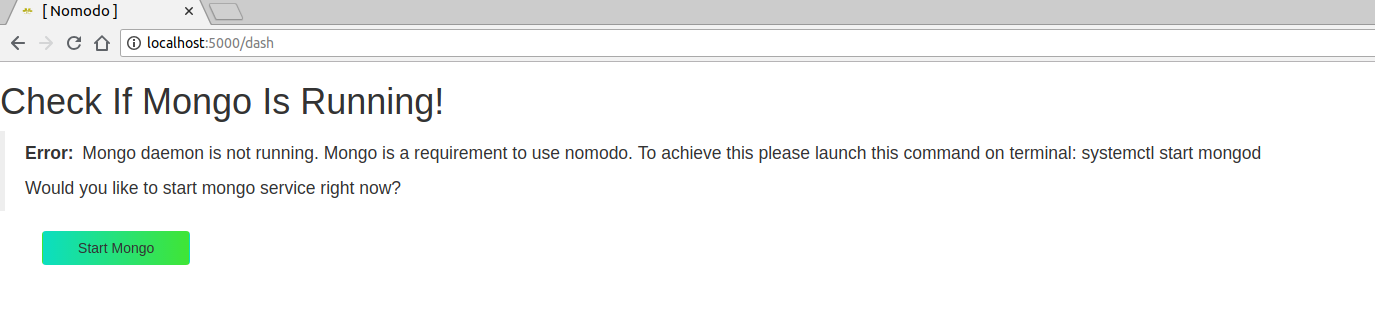
\includegraphics[width=\textwidth]{mongo.png}\\

\subsubsection{startMongo}\label{startMongo}
\begin{lstlisting}
@app.route('/startMongo', methods=['POST'])
def startMongo():
	try:
		error = None
		if request.form['startMongo'] == 'Start Mongo':
			log = mongostart()
			if(log['returncode'] != 0):
				error = log['stderr']
				return render_template('mongo.html',error=error)
			else:
				return redirect(url_for('dash'))
		else:
			error = 'Non funzica' 
			return render_template('mongo.html', error=error)
	except Exception:
		return internal_server_error(500)
\end{lstlisting}
Questo servizio viene richiamato nel modulo mongo.html. Il servizio è mappato come una richiesta di tipo POST, non accetta parametri in ingresso, però recupera il dato (scelto come hidden) in pagina attraverso l'oggetto form di request.
Il servizio richiama il metodo backend mongostart() e, in caso di successo, riinvia l'utente alla pagina principale, altrimenti mostra un errore in pagina.
Il meccanismo di logging all'utente è stati sviluppato utilizzando il message flashing.

\subsection{dash.html}\label{dash.html}

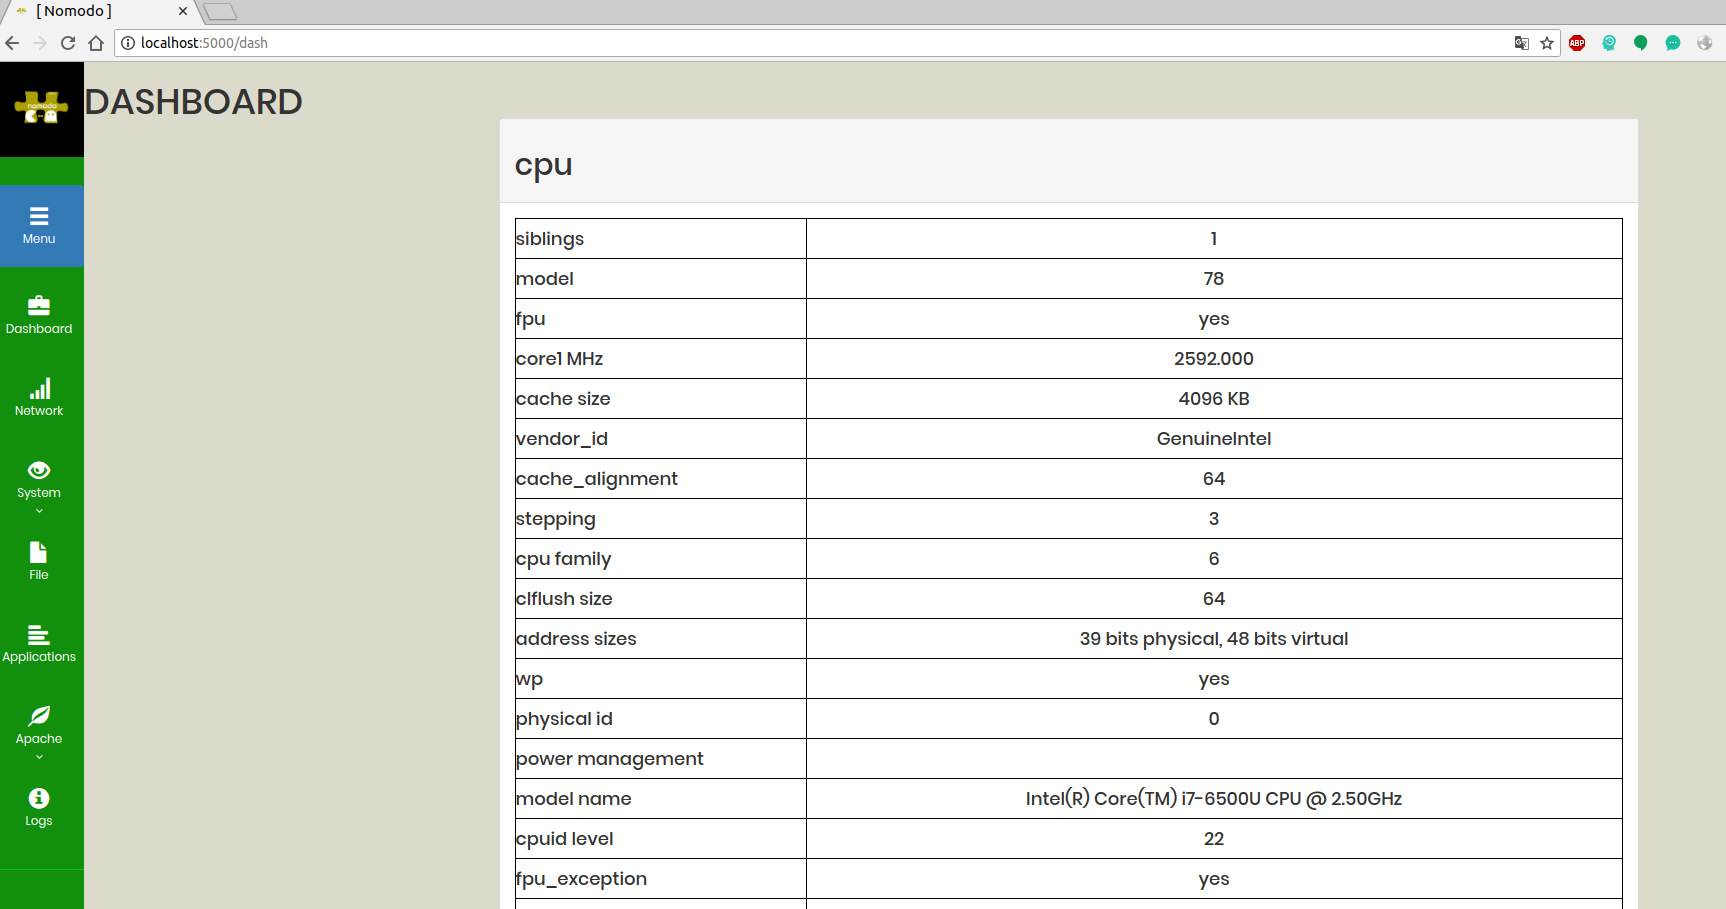
\includegraphics[width=\textwidth]{dash1.png}\\
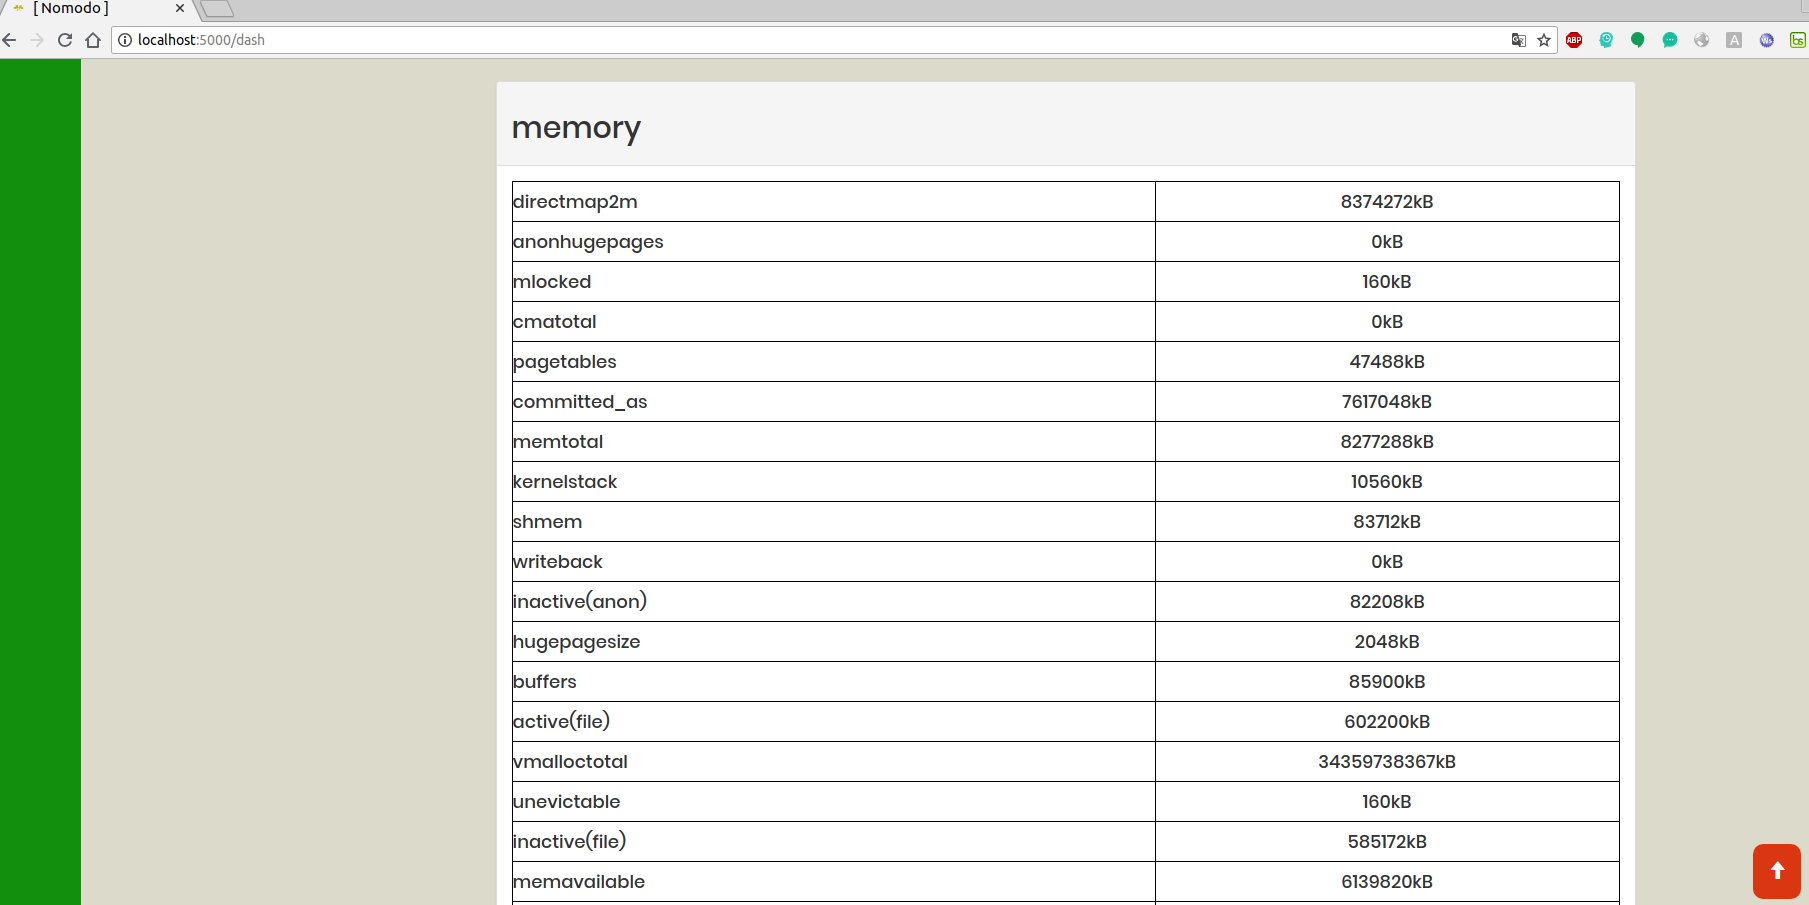
\includegraphics[width=\textwidth]{dash2.png}\\
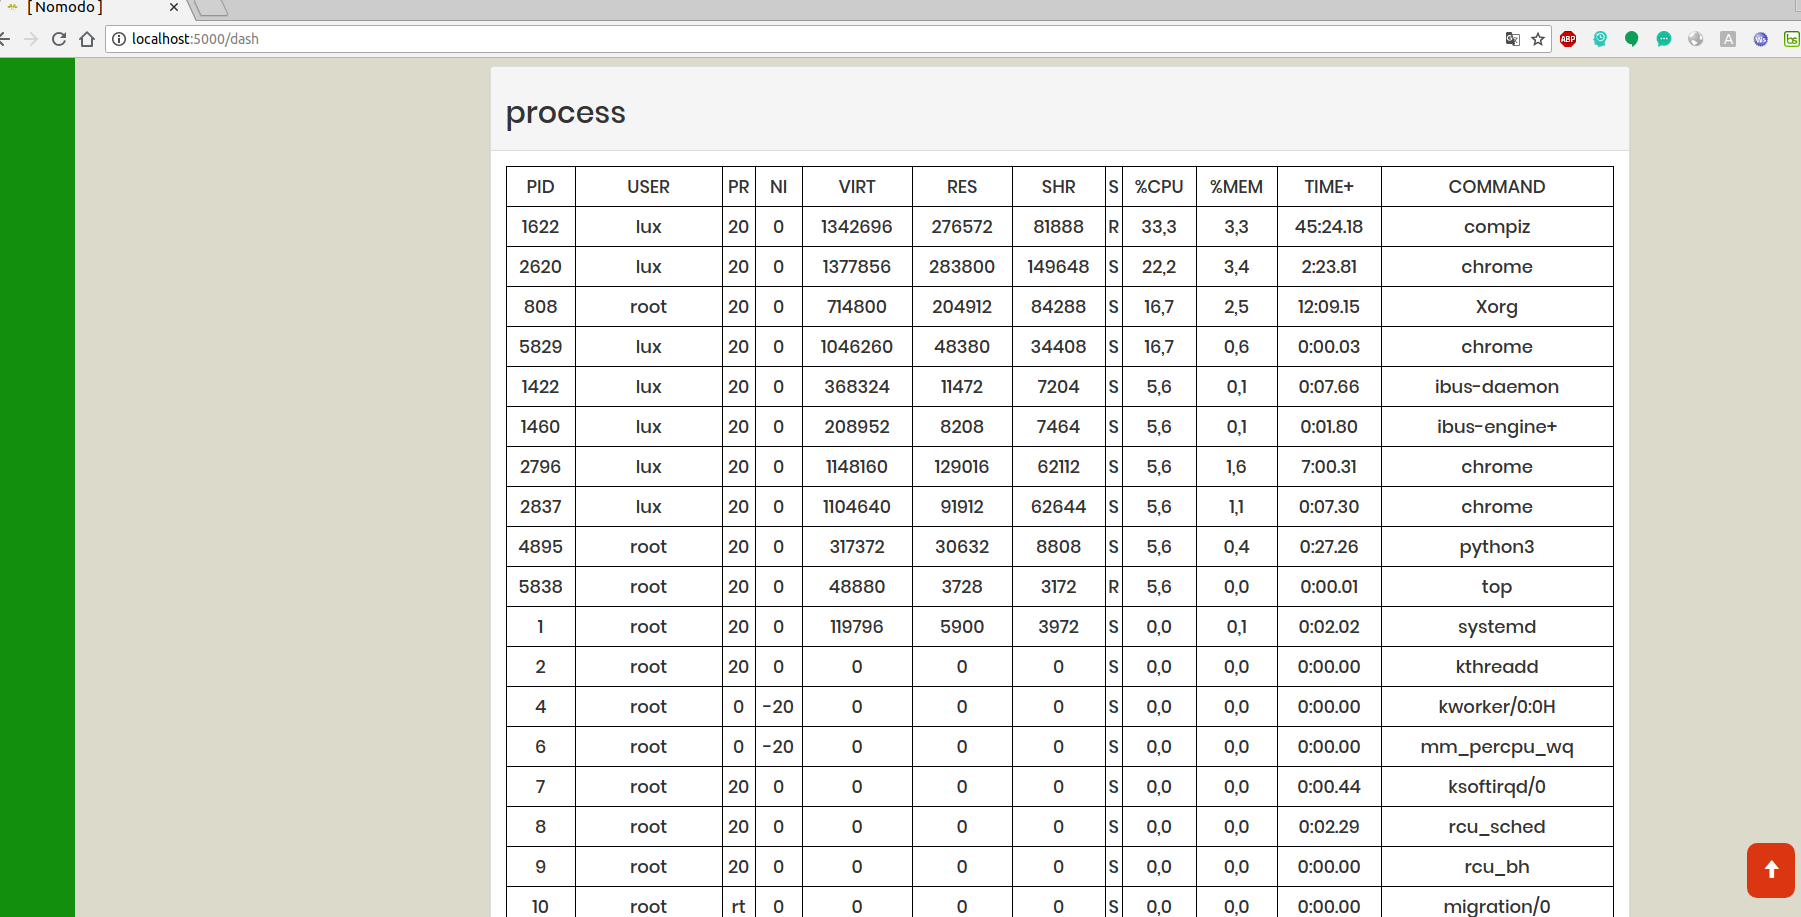
\includegraphics[width=\textwidth]{dash3.png}\\

\subsubsection{dash}\label{dash}
\begin{lstlisting}
@app.route('/dash')
def dash():
	tpl = getsysteminfo()
	(cpu,mem,proc) = tpl['data']
	return render_template('dash.html', cpu = cpu, mem = mem, proc = proc)
\end{lstlisting}
Il servizio richiama il metodo getsysteminfo(), che restituisce in output una tupla con le informazioni sulla cpu, sulla memoria e sui processi e li mostra nella pagina dash.html.

\subsection{network.html}\label{network.html}

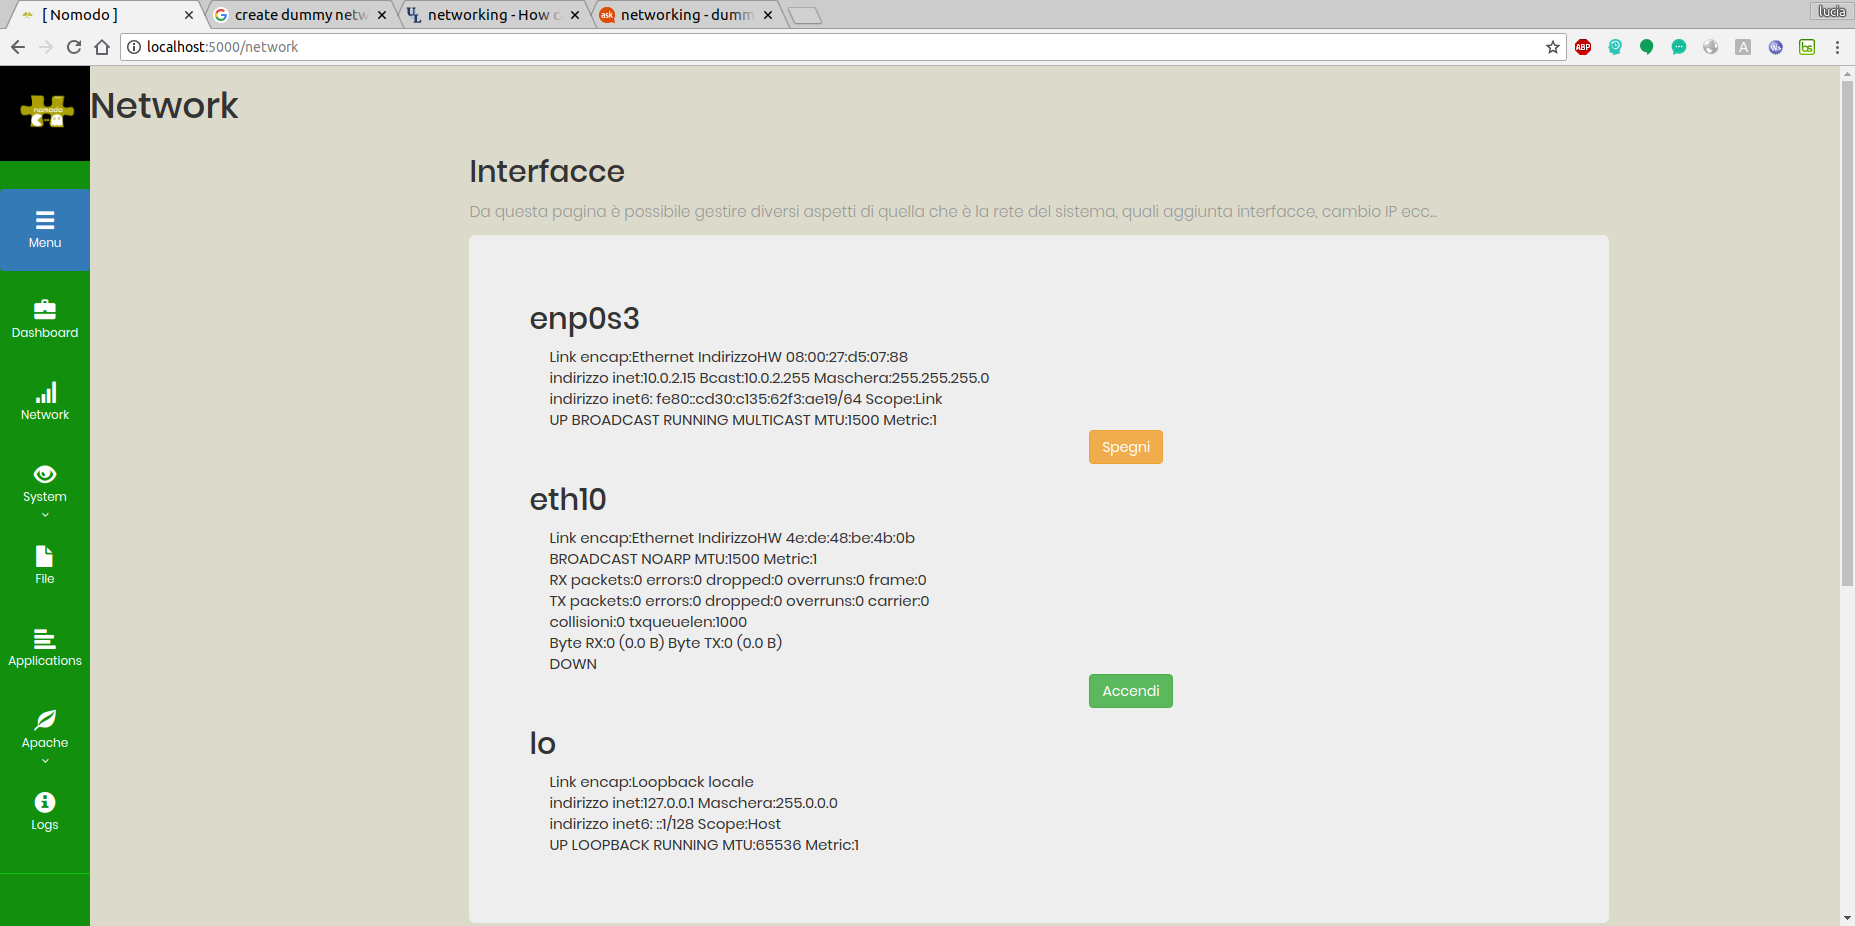
\includegraphics[width=\textwidth]{network1.png}\\
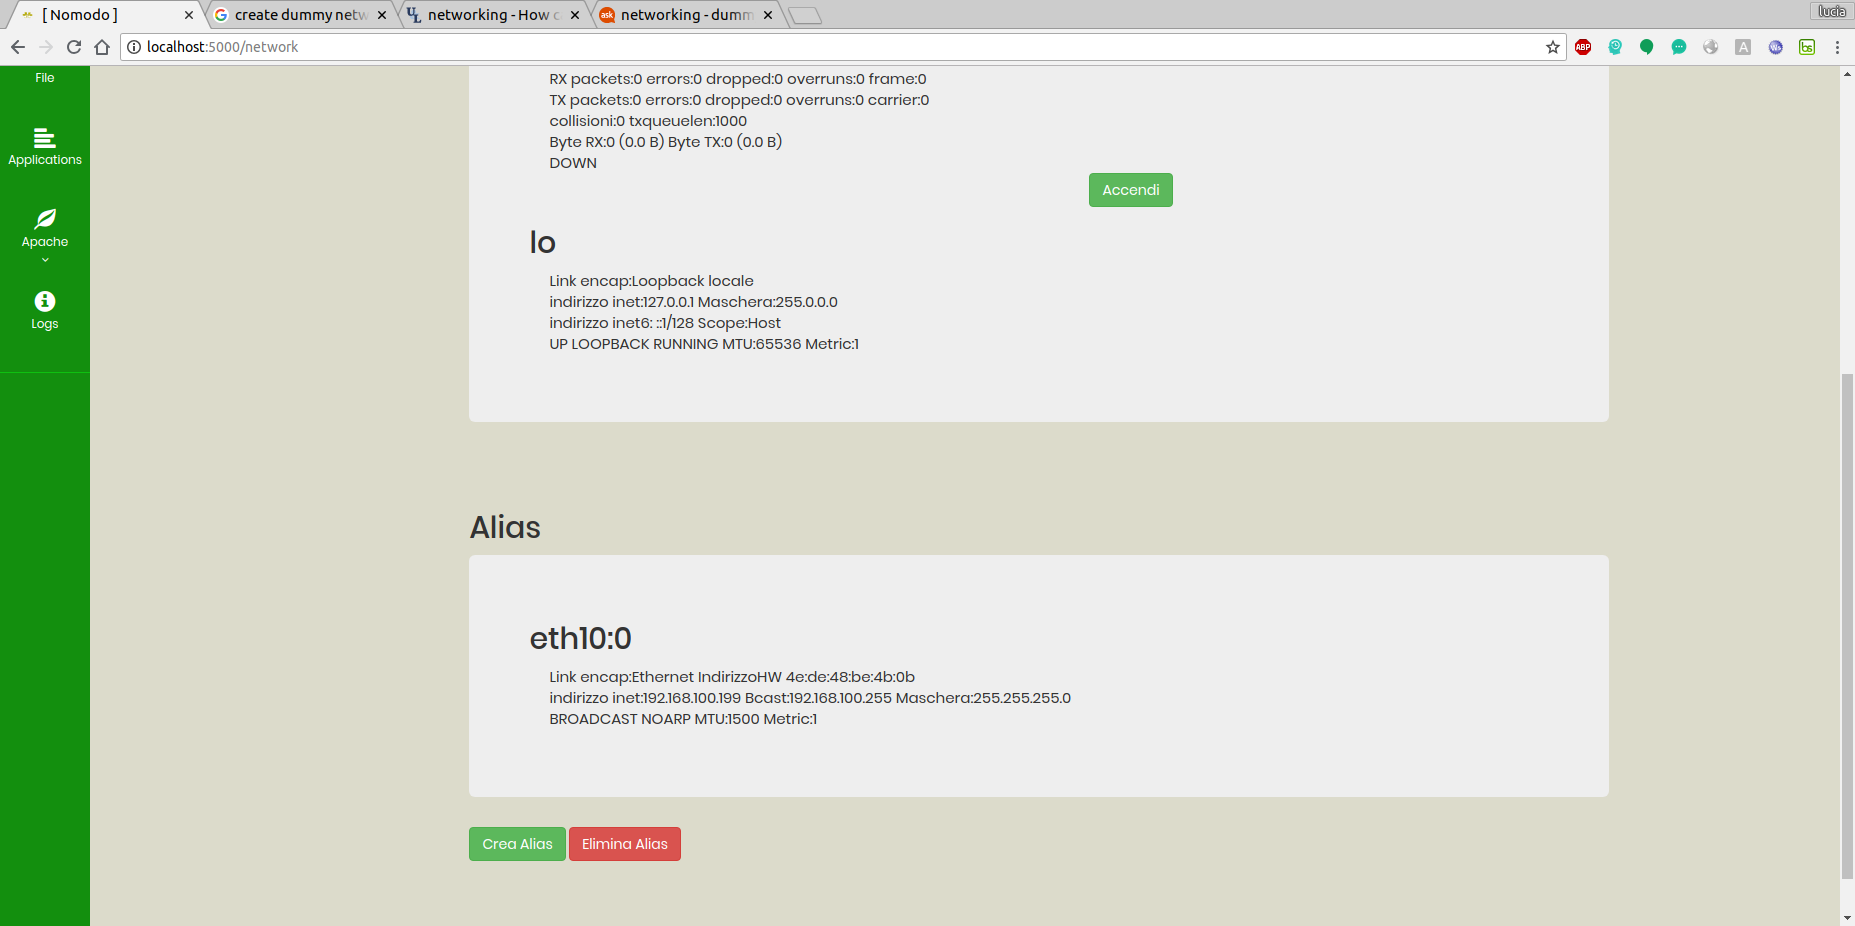
\includegraphics[width=\textwidth]{network2.png}\\

\subsubsection{network}\label{network}
\begin{lstlisting}
@app.route('/network')
def network():
	key_remove = list()
	lo = dict()
	als = dict()
	faceUp = dict()
	faceDown = dict()
	facestat = ifacestat()['data']
	for key,value in facestat.items():
		if 'LOOPBACK' in value[-1]:
			lo.update({key:facestat[key]})
			key_remove.append(key)
		elif ':' in key:
			als.update({key:facestat[key]})
			key_remove.append(key)

	for key in key_remove:
		del facestat[key]
	
	for key, value in facestat.items():
		if not 'UP' in value[-1]:
			facestat[key].append('DOWN')
	return render_template('network.html', facestat=facestat, lo=lo, als=als)
\end{lstlisting}
Il servizio di network mostra in pagina le interfacce si sistema disponibili. L'elaborazione del servizio è più complessa perchè i dati ricevuti dal metodo ifacestat() sono stati divisi in base a diversi controlli:
\begin{itemize}
\item{se tra i valori dell'interfaccia analizzata nel ciclo è presente la parola loopback (cioè se è l'interfaccia che identifica la macchina locale) viene salvata in un nuovo dizionario e la chiave che rappresenta l'interfaccia viene eliminata dal dizionario iniziale.}
\item{se nella chiave  che identifica il nome dell'interfaccia, sono presenti i ':', allora si tratta di un alias e viene salvata in un nuovo dizionario e eliminata la chiave dal dizionario iniziale.}
\end{itemize}
Lo sviluppo è stato deciso in questo modo perchè in pagina venivano fatti dei controlli su bottoni diversi in base all'entità esaminata.

\subsubsection{createAlias}\label{createAlias}
\begin{lstlisting}
@app.route('/createAlias', methods=['POST'])
def createAlias():
	try:
		error = None
		iface = request.form['iface']
		address = request.form['address']
		netmask = request.form['netmask']
		broadcast = request.form['broadcast']
		if not iface or iface == '-- Seleziona interfaccia --':
			error = 'Invalid option'
		else:
			generatedAliasName = getnewifacealiasname(iface)
			if not address:
				error = 'Address empty'
			else:
				log = createalias(generatedAliasName['data'],address,netmask,broadcast)
				if(log['returncode'] != 0):
					error = log['stderr']
				else:
					flash("Alias created correctly")
					return redirect(url_for('network'))
		return render_template('network.html', error=error)
	except Exception:
		return internal_server_error(500)
\end{lstlisting}
Il servizio è mappato come una richiesta di tipo POST non accetta parametri in ingresso, però recupera i parametri dal modello network.html. Una volta verificato che i parametri della request sono validi, utilizza la funzione getnewifacealiasname() per la generazione dell'nome dell'alias per poi chiamare la funzione createalias() che accetta in ingresso 4 parametri: nome dell'interfaccia generata, l'indirizzo, la netmask e l'indirizzo di broadcast.
Questa funzione viene applicata per le interfacce che non rappresentano la macchina locale e non sono alias.

\subsubsection{destroyAlias}\label{destroyAlias}
\begin{lstlisting}
@app.route('/destroyAlias', methods=['POST'])
def destroyAlias():
	try:
		error = None
		alias = request.form['alias']
		if not alias or alias == '-- Seleziona alias --':
			error = 'Invalid option'
		else:
			log = destroyalias(alias)
			if(log['returncode'] != 0):
				error = log['stderr']
			else:
				flash("Alias deleted correctly")
				return redirect(url_for('network'))
		return render_template('network.html', error=error)
	except Exception:
		return internal_server_error(500)
\end{lstlisting}
Il servizio è mappato come una richiesta di tipo POST e non accetta parametri in ingresso. I parametri vengono recuperati dal modello tramite la request e viene passata alla funzione backend destroyalias() che serve a cancellare l'alias.

\subsubsection{upIface}\label{upIface}
\begin{lstlisting}
@app.route('/upIface', methods=['POST'])
def upIface():
	iface = request.form['iface']
	address = request.form['address']
	netmask = request.form['netmask']
	broadcast = request.form['broadcast']
	facestat = ifacestat()['data']
	if '-- Seleziona interfaccia --' in iface:
		flash('Invalid option')
	else:
		if iface in facestat:
			log = ifaceup(iface)
			if(log['returncode'] != 0):
				error = log['stderr']
			else:
				flash("Interface up!")
				return redirect(url_for('network'))			
	return render_template('network.html', error=error)
\end{lstlisting}
Il servizio è mappato come una richiesta di tipo POST e non accetta parametri in ingresso. I parametri vengono recuperati dal modello tramite la request.
Viene richiamato nuovamente getnewifacealiasname() per verificare che l'iface scelto esista tra gli iface e nel caso in cui lo fosse viene richiamata la funziona ifaceup() che porta su l'interfaccia.

\subsubsection{downIface}\label{downIface}
\begin{lstlisting}
@app.route('/downIface/<string:iface>', methods=['POST'])
def downIface(iface):
	error = None
	if request.form['down'] == 'Spegni':
		log = ifacedown(iface)
		if(log['returncode'] != 0):
			error = log['stderr']
		else:
			flash('Interface down!')
			return redirect(url_for('network'))
	else:
		error = 'Non funzica' 
	return render_template('network.html', error=error)
\end{lstlisting}
Il servizio è mappato come una richiesta di tipo POST e accetta un solo parametro in ingresso che corrisponde al nome dell'iface. Il parametro viene poi passato alla funzione ifacedown() che porta giù l'interfaccia.

\subsection{param.html}\label{param.html}

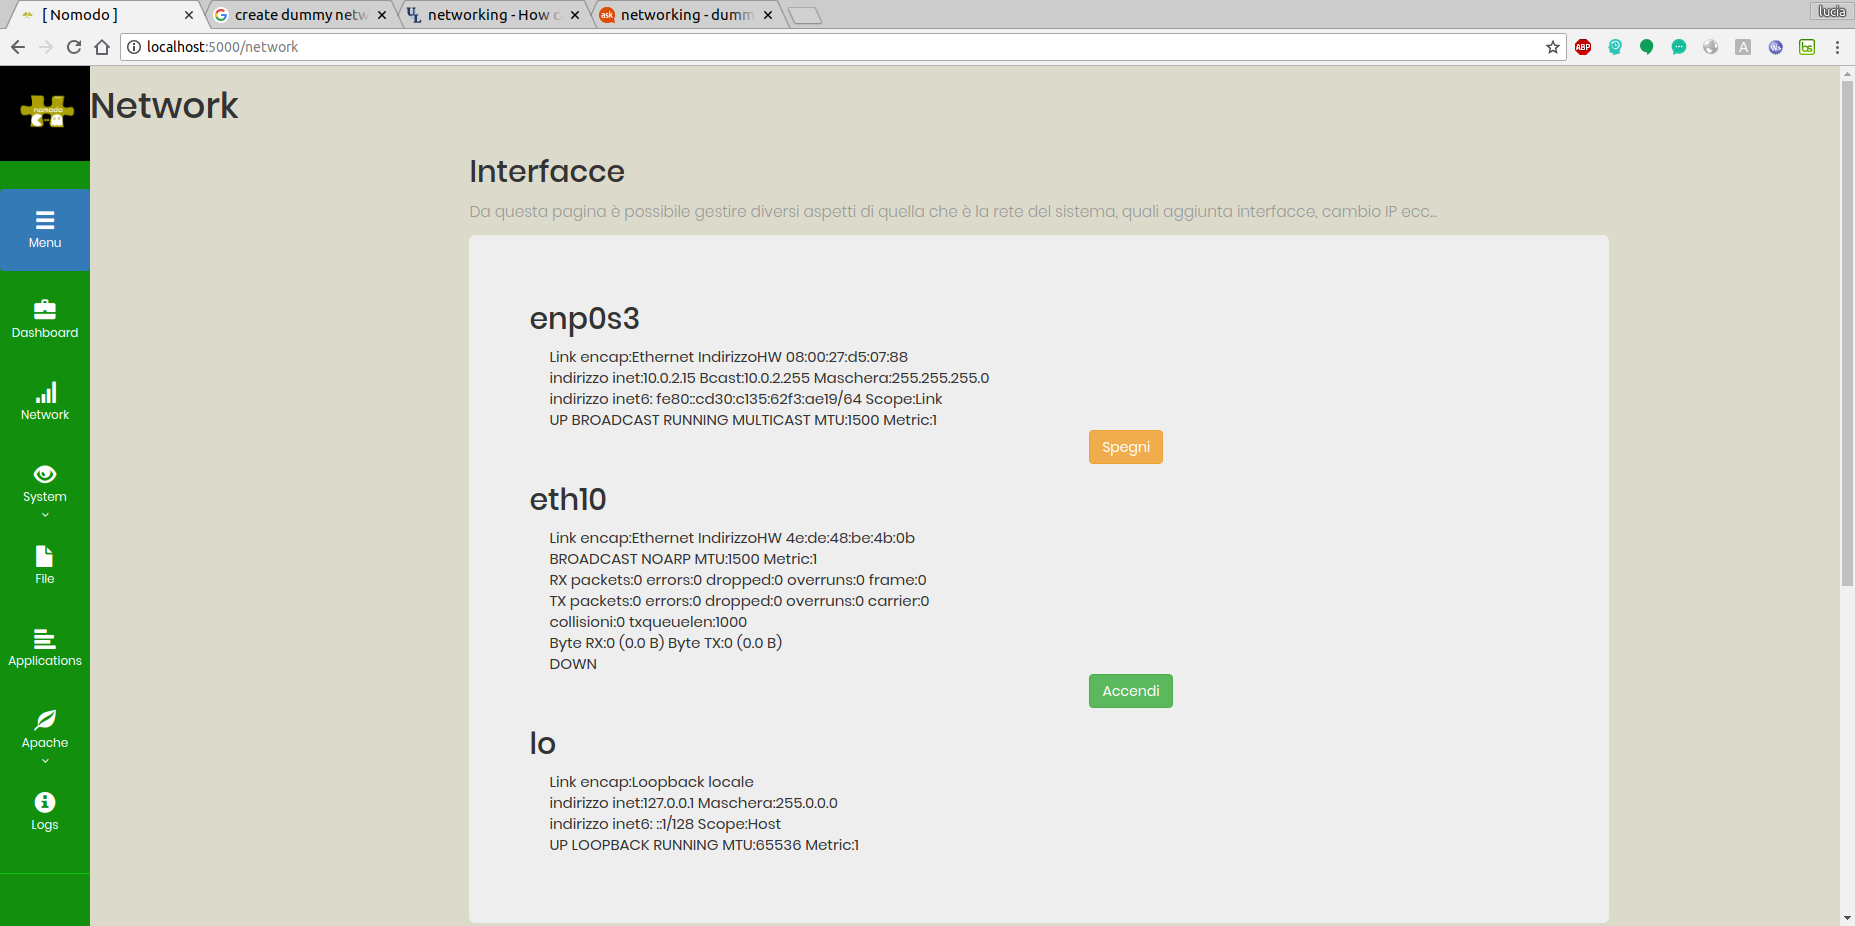
\includegraphics[width=\textwidth]{network1.png}\\
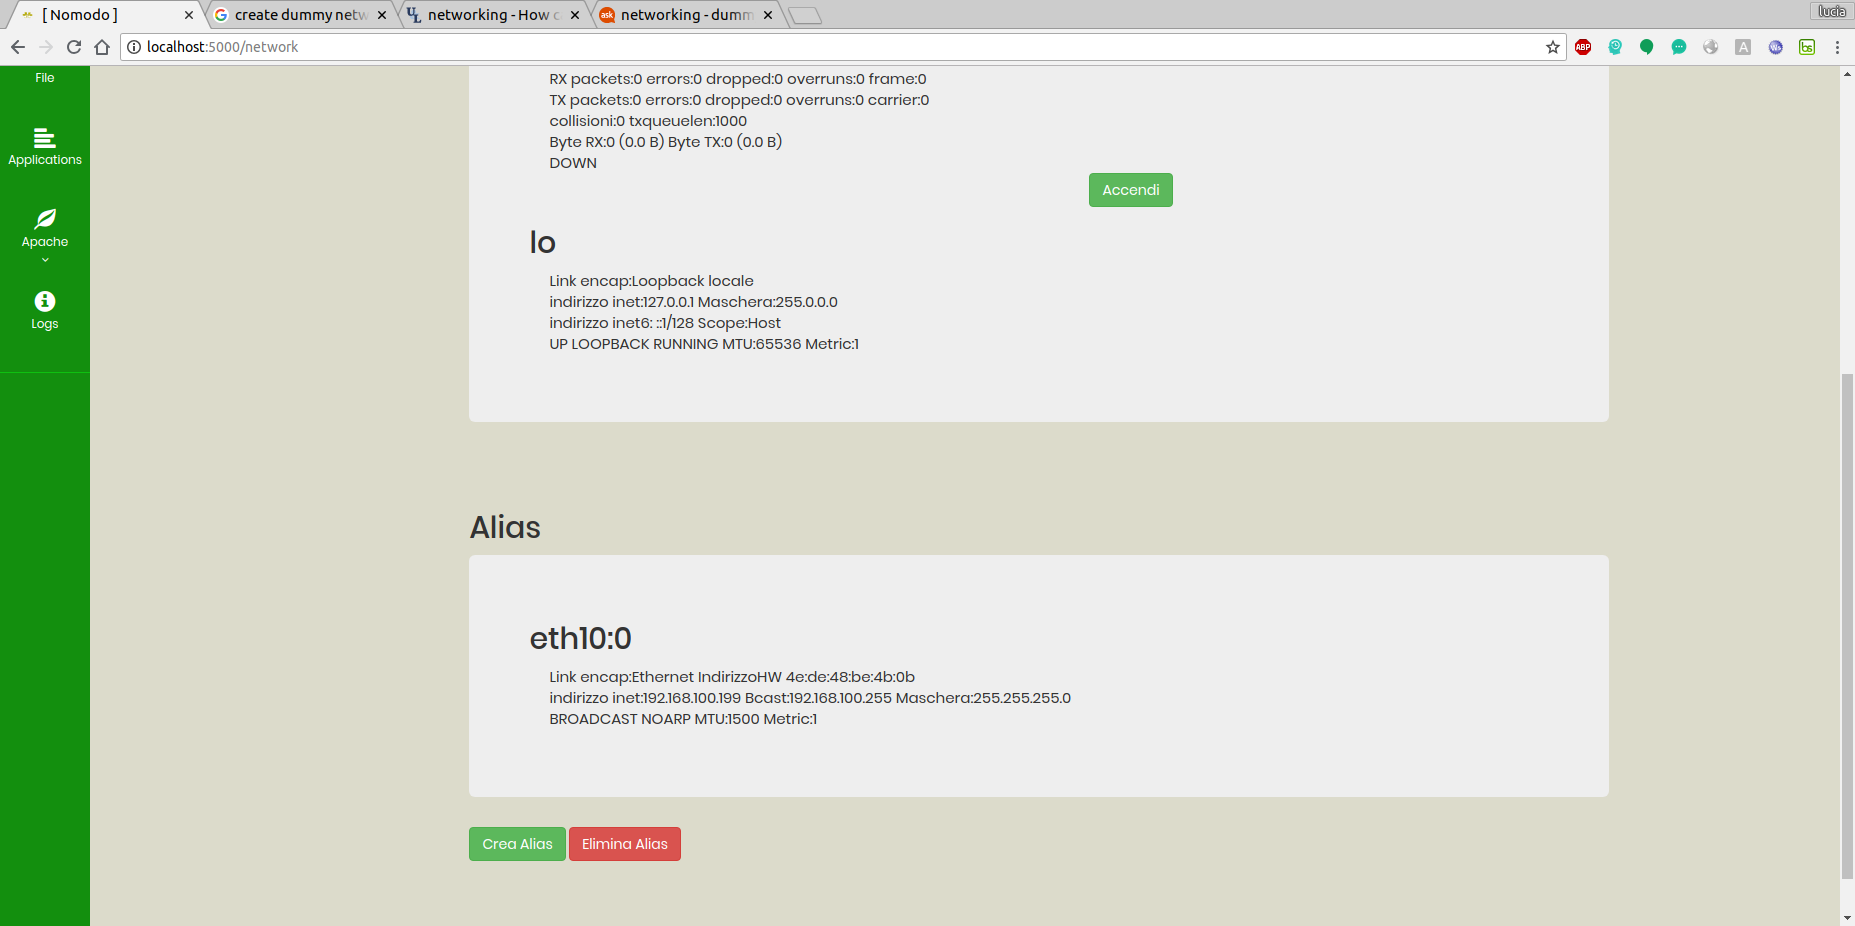
\includegraphics[width=\textwidth]{network2.png}\\


\end{document}
